%%%%%%%%%%%%%%%%%%%%%%%%%%%%%%%%%%%%%%%%%%%%%%%%%%%
%% LaTeX book template                           %%
%% Author:  Amber Jain (http://amberj.devio.us/) %%
%% License: ISC license                          %%
%%%%%%%%%%%%%%%%%%%%%%%%%%%%%%%%%%%%%%%%%%%%%%%%%%%

\documentclass[a4paper,11pt,oneside]{book}
\usepackage[T1]{fontenc}
\usepackage[utf8]{inputenc}
\usepackage{lmodern}
%%%%%%%%%%%%%%%%%%%%%%%%%%%%%%%%%%%%%%%%%%%%%%%%%%%%%%%%%
% Source: http://en.wikibooks.org/wiki/LaTeX/Hyperlinks %
%%%%%%%%%%%%%%%%%%%%%%%%%%%%%%%%%%%%%%%%%%%%%%%%%%%%%%%%%
\usepackage{hyperref}
\usepackage{graphicx}
\usepackage[english]{babel}
\usepackage{bm}
\usepackage{amsfonts}
\usepackage{amsmath}
\usepackage{enumerate}
\newcommand{\numpy}{{\tt numpy}}    % tt font for numpy
\usepackage{algorithm}
\usepackage{algorithmicx}
\usepackage{algpseudocode}
\usepackage{subfigure}
\renewcommand{\algorithmicrequire}{\textbf{Input:}} % Use Input in the format of Algorithm
\renewcommand{\algorithmicensure}{\textbf{Output:}} % Use Output in the format of Algorithm
\newtheorem{theorem}{\bf Theorem}[chapter]
\newtheorem{definition}[theorem]{Definition}
\newtheorem{proposition}[theorem]{Proposition}
\newtheorem{remark}[theorem]{Remark}
\newenvironment{proof}{{\noindent\it Proof}\quad}{\hfill $\square$ \par}
%%%%%%%%%%%%%%%%%%%%%%%%%%%%%%%%%%%%%%%%%%%%%%%%%%%%%%%%%%%%%%%%%%%%%%%%%%%%%%%%
% 'dedication' environment: To add a dedication paragraph at the start of book %
% Source: http://www.tug.org/pipermail/texhax/2010-June/015184.html            %
%%%%%%%%%%%%%%%%%%%%%%%%%%%%%%%%%%%%%%%%%%%%%%%%%%%%%%%%%%%%%%%%%%%%%%%%%%%%%%%%
\newenvironment{dedication}
{
   \cleardoublepage
   \thispagestyle{empty}
   \vspace*{\stretch{1}}
   \hfill\begin{minipage}[t]{0.66\textwidth}
   \raggedright
}
{
   \end{minipage}
   \vspace*{\stretch{3}}
   \clearpage
}

%%%%%%%%%%%%%%%%%%%%%%%%%%%%%%%%%%%%%%%%%%%%%%%%
% Chapter quote at the start of chapter        %
% Source: http://tex.stackexchange.com/a/53380 %
%%%%%%%%%%%%%%%%%%%%%%%%%%%%%%%%%%%%%%%%%%%%%%%%
\makeatletter
\renewcommand{\@chapapp}{}% Not necessary...
\newenvironment{chapquote}[2][2em]
  {\setlength{\@tempdima}{#1}%
   \def\chapquote@author{#2}%
   \parshape 1 \@tempdima \dimexpr\textwidth-2\@tempdima\relax%
   \itshape}
  {\par\normalfont\hfill--\ \chapquote@author\hspace*{\@tempdima}\par\bigskip}
\makeatother

%%%%%%%%%%%%%%%%%%%%%%%%%%%%%%%%%%%%%%%%%%%%%%%%%%%
% First page of book which contains 'stuff' like: %
%  - Book title, subtitle                         %
%  - Book author name                             %
%%%%%%%%%%%%%%%%%%%%%%%%%%%%%%%%%%%%%%%%%%%%%%%%%%%

% Book's title and subtitle
\title{\huge \textbf{Computational Intelligence Lab 2020}}
% Author
\author{\textsc{Yu Fei}}



\begin{document}

\frontmatter
\maketitle

%%%%%%%%%%%%%%%%%%%%%%%%%%%%%%%%%%%%%%%%%%%%%%%%%%%%%%%%%%%%%%%
% Add a dedication paragraph to dedicate your book to someone %
%%%%%%%%%%%%%%%%%%%%%%%%%%%%%%%%%%%%%%%%%%%%%%%%%%%%%%%%%%%%%%%
%\begin{dedication}
%Dedicated to Calvin and Hobbes.
%\end{dedication}

%%%%%%%%%%%%%%%%%%%%%%%%%%%%%%%%%%%%%%%%%%%%%%%%%%%%%%%%%%%%%%%%%%%%%%%%
% Auto-generated table of contents, list of figures and list of tables %
%%%%%%%%%%%%%%%%%%%%%%%%%%%%%%%%%%%%%%%%%%%%%%%%%%%%%%%%%%%%%%%%%%%%%%%%
\tableofcontents
%\listoffigures
%\listoftables

\mainmatter

%%%%%%%%%%%%%%%%
% NEW CHAPTER! %
%%%%%%%%%%%%%%%%
\chapter{Linear Autoencoder}

%\begin{chapquote}{Author's name, \textit{Source of this quote}}
%``This is a quote and I don't know who said this.''
%\end{chapquote}
\section{Dimension Reduction}
In machine learning, when we work with data, we often start with very high-dimensional representation (raw data), like mega-pixel images or raw audio data. A question raises naturally is that is it really necessary to have so many dimensions to describe our data. This motivates this field of dimension reduction. Actually dimension reduction lies in the heart of many fields in machine learning and data science:
\begin{itemize}
    \item visualization - e.g. 2D or 3D
    \item data compression - fewer coefficients
    \item signal recovery - discard irrelevant information(noise)
    \item discover modes of variation - intrinsic properties of data
    \item feature discovery - learn better representations
    \item generative models - latent variables (knowing low-dim representation often helps to synthesize data)
\end{itemize}
\par For a typical dimension reduction problem, what we are given are $n$ high-dimension data points$\{\bm{x}_i\in\mathbb{R}^{m}\},\ i=1,\dots,n$.
We want to find low-dimensional representation $\{\bm{z}_i\in \mathbb{R}^k\}$ for $\{\bm{x}_i\},\ i=1,\dots,n$ in a predefined reduced dimension number $k\ll m$.
\par An example for dimension reduction is the Eigenfaces method for face images. A 2D pixel face image $\bm{x}_i\in \mathbb{R}^{100\times 100}$ after vectorization is a vector in $\mathbb{R}^{10000}$. Eigenfaces suggests to approximate each face with a weighted superposition of few (say 4) basis images. The 4 coefficients are our desired low-dimensional representation for a given image. The fact that we can approximate a face image well with a few basis images also indicates that we have understood something like statistical properties about faces.

\subsection{Linear Dimension Reduction}
In Linear dimension reduction, the relation between the low-dimensional representation $\bm{z}_i$ and its corresponding $\bm{x}_i$ is governed by some (fixed) matrix $C$:
\begin{equation*}
    \bm{z}_i = C\bm{x}_i,\ C\in\mathbb{R}^{k\times m}
\end{equation*}
where we can regard $C$ as a linear map $\mathbb{R}^m\rightarrow \mathbb{R}^k$. Each entry of the feature vector $\bm{z}$ is a linear combination of input variables
\begin{equation*}
    \bm{z} = C\bm{x} \Longleftrightarrow z_r = \sum_{s=1}^{m} c_{rs}x_s\ \forall r\in [k],\ C=(c_{rs})
\end{equation*}
\par In neural network terminology, each $z_r$ is a \emph{linear unit} that computes a linear function of its inputs with weight vector $\bm{c}_r = (c_{r1},\dots,c_{rm})^T\in \mathbb{R}^m$, which is the r-th row of $C$.
\par Now we take a neural network view. Think about a (deep) neural network as in Figure \ref{fig_1_1}. In supervised learning, given targets $\bm{y}$ and the inputs $\bm{x}$, the training of such a neural network can be seen as learning (better) representations along the way. The activation of middle layers with fewer dimensions are ideal low-dim representations for the original input. Although this view from neural network gives some interesting insights, in this chapter we will focus on the unsupervised learning case, where we don't have access to such targets for our $\bm{x}$.
\begin{figure}[h]
\centering
\begin{minipage}[t]{0.5\linewidth}
\centering
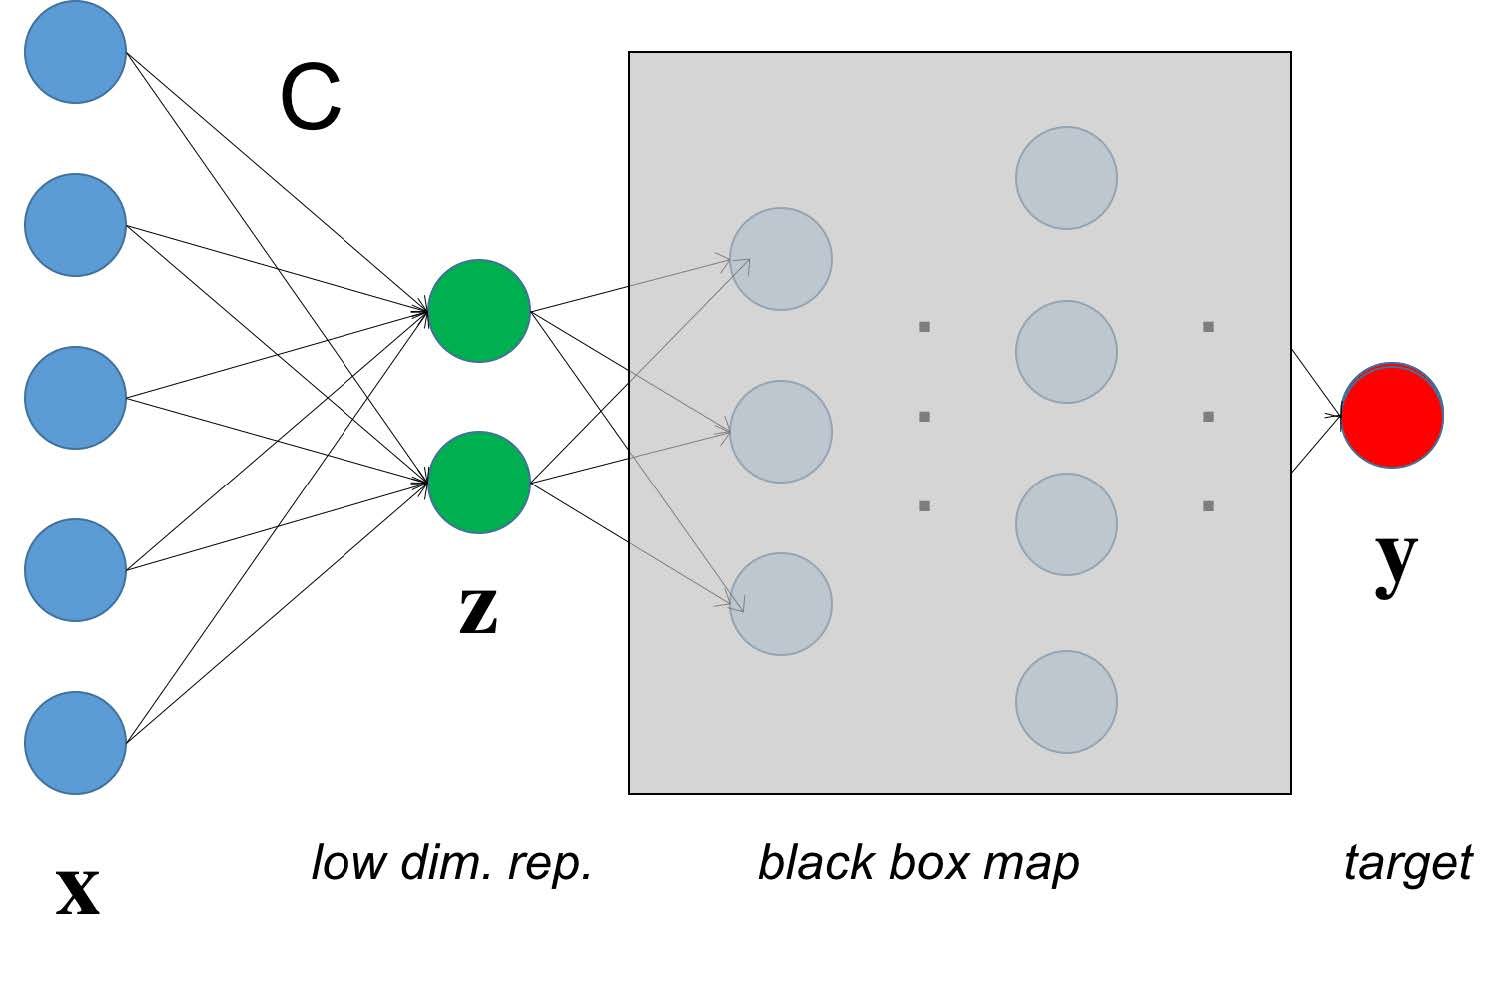
\includegraphics[width=5.5cm]{fig_1_1.jpg}
\caption{Dimension reduction from a neural network view}\label{fig_1_1}
\end{minipage}
\begin{minipage}[t]{0.4\linewidth}       
\centering
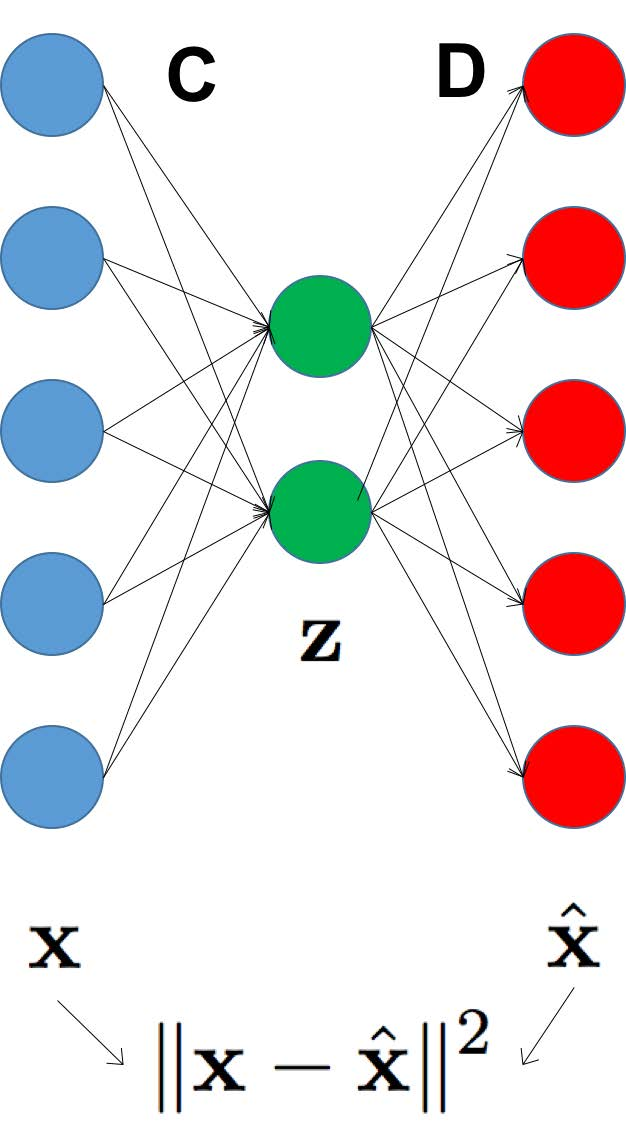
\includegraphics[width=2.5cm]{fig_1_2.jpg}
\caption{Linear Autoencoder}\label{fig_1_2}
\end{minipage}
\end{figure}
\section{Linear Autoencoder}
A Linear autoencoder can be represented neural network with 1 hidden layer without activation function (Figure \ref{fig_1_2}). The idea of linear autoencoder is to learn the low-dim representation by learning an identity map. This is done in a \emph{fully unsupervised} way. Specifically, we first map the input linearly to a lower dimension, then use a linear reconstruction to recover the original input. The parameters $\theta$ of a linear autoencoder consist of two parts: an encoder matrix $C\in \mathbb{R}^{k\times m}$ and a decoder matrix $D\in \mathbb{R}^{m\times k}$ which is a linear reconstruction map. Given the input $\bm{x}$ and the model parameters $\theta$, the output of the linear autoencoder can therefore be written as $\hat{\bm{x}}(\theta)=DC\bm{x}$. The criteria people often use to evaluate the reconstruction is the squared reconstruction loss:
\begin{equation*}
    l(\bm{x};\theta)=\frac{1}{2}\|\bm{x}-\hat{\bm{x}}(\theta)\|^2
\end{equation*}
\par Since we often don't care about the order of entries in $\bm{x}$, linear autoencoders are trained with sample reconstruction error:
\begin{equation*}
    J(\theta)=\frac{1}{n}\sum_{i=1}^{n}l(\bm{x}_i;\theta)
\end{equation*}
\par By optimizing over $J(\theta)$, a linear autoencoder learn an approximate identity map over a specific data distribution, and the \emph{bottleneck} layer $\bm{z}$ is the desired low-dim representation.

\begin{remark}
By definition, as long as $k<m$, an autoencoder in Figure \ref{fig_1_2} cannot learn an identity map for everything in $\mathbb{R}^m$, but fortunately we only care about inputs from a specific distribution. 
\end{remark}

\par Mathematically, the linear autoencoder defines a linear map 
\begin{equation*}
    F:\mathbb{R}^m \rightarrow \mathbb{R}^m,\ F:=DC
\end{equation*}
Ideally, we want $F$ to be approximately an identity map, i.e. $F\approx I$. However, the bottleneck places an upper bound on the rank of $F$, making $F$ a \emph{low-rank approximation} of the identity map over a specific data distribution.
\par The \emph{rank} of a linear map $A:\mathbb{R}^k\rightarrow \mathbb{R}^l$ is defined as the dimension of the image of $A$:
\begin{equation*}
    rank(A):=dim(im(A))\leq min\{k,l\}
\end{equation*}
Note that the ranks of matrices and the rank of their product satisfy
\begin{equation*}
    rank(AB)\leq \min\{rank(A), rank(B)\}
\end{equation*}
and that a matrix $M$ has a decomposition $M=AB$ with $A\in \mathbb{R}^{m\times k},B\in \mathbb{R}^{k\times n}$, if and only if $rank(M)\leq k$:
\begin{equation*}
    \exists A\in \mathbb{R}^{m\times k},\ B\in \mathbb{R}^{k\times n},\ M=AB \Longleftrightarrow rank(M)\leq k
\end{equation*}
Then the low-rank approximation $F$ that linear autoencoder performs satisfies
\begin{equation*}
    rank(F)\leq \min\{rank(C),rank(D)\}\leq k
\end{equation*}
\par At this point, we can already try to solve this problem using methods like training a neural network to find $C$ and $D$. However, if possible, we'd like to gain some understanding about the theoretical limit that the reconstruction quality can achieve. To answer this question, we introduce some extra notation and concepts first.
\par By writing data and the corresponding approximations in matrix forms $X = [\bm{x}_1\dots \bm{x}_n],\ \hat{X} = [\hat{\bm{x}}_1\dots \hat{\bm{x}}_n]$, we can rewrite the error function:
\begin{equation*}
    J(\theta)=\frac{1}{2n}\sum_{i=1}^{n}\|\bm{x}-\hat{\bm{x}}(\theta)\|^2=\frac{1}{2n}\|X-\hat{X}(\theta)\|^2_F
\end{equation*}
where $\|A\|_F:=\|vec(A)\|_2=\sqrt{\sum_{ij}a_{ij}^2}$ is the Frobenius norm. Then optimizing $J(\theta)$ over all possible matrix $C$ and $D$ is equivalent to solving a standard low-rank approximation problem.
\begin{definition}
Given $X\in \mathbb{R}^{m\times n}$ and a rank constraint $k$. Low-rank approximation problem with fit measured by the Frobenius norm is defined as:
\begin{equation*}
    \mathop{{\rm minimize}}_{\hat{X}:\ rank(\hat{X})\leq k}\ \|X-\hat{X}\|_F
\end{equation*}
\end{definition}
\par The Eckart-Young theorem gives a bound on the reconstruction error of low-rank approximation problem and also a analytic solution that can achieve this bound.
\begin{theorem}\label{thm_1_EY}
(Eckart-Young) Let $A\in \mathbb{R}^{m\times n}$ be a real matrix, for $k\leq \min\{m,n\}$:
\begin{equation*}
    \|A-U\Sigma_kV^T\|_F^2 = \min_{\hat{A}:\ rank(\hat{A})\leq k}\|A-\hat{A}\|^2_F = \sum_{l=k+1}^{\min\{m,n\}}\sigma_l^2 
\end{equation*}
where $A=U\Sigma V^T$ is the singular value decomposition of $A$ and $\Sigma_k$ is the truncated diagonal matrix of singular values.
\end{theorem}
\begin{proof}
Without loss of generality, we assume that $m\geq n$. $\Sigma$ is an $m\times n$ diagonal matrix with entries $(\sigma_1,\dots,\sigma_n)$ such that $\sigma_1\geq\dots\geq \sigma_n\geq 0$.
\par To prove Eckart-Young Theorem for Frobenius Norm, we first prove the theorem for spectral norm. We claim that the best rank $k$ approximation of $A$ in the spectral norm is given by
\begin{equation*}
    A_k = \sum_{i=1}^{k}\sigma_i\bm{u}_i\bm{v}^T_i
\end{equation*}
where $\bm{u}_i$ and $\bm{v}_i$ are columns of $U$ and $V$, respectively. Since we have
\begin{equation*}
    \|A-A_k\| = \left\|\sum_{i=k+1}^{n}\sigma_i\bm{u}_i\bm{v}^T_i\right\| = \sigma_{k+1}
\end{equation*}
Therefore all we need to show is given any rank k reconstruction $B_k=XY^T$, where $X,Y\in \mathbb{R}^{m\times k}$, it satisfies
\begin{equation*}
     \|A-A_k\| =\sigma_{k+1}\leq \|A-B_k\|
\end{equation*}
Since $Y$ has $k$ columns, there exists a linear combination $\bm{w}$ of $\{\bm{v}_1,\dots,\bm{v}_{k+1}\}$ such that
\begin{equation*}
    \bm{w} = \sum_{i=1}^{k+1}\alpha_i\bm{v}_i,\ Y^T\bm{w}=0,\ \|\bm{w}\|=1
\end{equation*}
therefore we obtain
\begin{equation*}
    \|A-B_k\|^2\geq \|(A-B_k)\bm{w}\|^2 = \|A\bm{w}\|^2 = \sum_{i=1}^{k+1}\alpha_i^2\sigma_i^2\geq \sigma_{k+1}^2\sum_{i=1}^{k+1}\alpha_i^2 = \sigma_{k+1}^2
\end{equation*}
which concludes the proof for spectral norm.
\par For Frobenius norm, since
\begin{equation*}
    \|A-A_k\|_F^2= \left\|\sum_{i=k+1}^{n}\sigma_i\bm{u}_i\bm{v}^T_i\right\|_F^2 = \sum_{i=k+1}^{n}\sigma_i^2
\end{equation*}
all we have to prove is given any rank k reconstruction $B_k=XY^T$, where $X,Y\in \mathbb{R}^{m\times k}$, it satisfies
\begin{equation*}
     \|A-A_k\| =\sum_{i=k+1}^{n}\sigma_i^2\leq \|A-B_k\|
\end{equation*}
\par Assume $A=A'+A''$. $A'_k$ and $A''_k$ are the corresponding rank k reconstruction given by SVD of $A'$ and $A''$ respectively. Then $\forall 1\leq i,j\leq n$
\begin{align*}
    \sigma_i(A')+\sigma_j(A'') &= \sigma_1(A'-A'_{i-1})+\sigma_1(A''-A''_{j-1})\\
    &\geq \sigma_1(A-A'_{i-1}-A''_{j-1})\ (\text{Triangle ineq. of spectral norm})\\
    &\geq \sigma_1(A-A_{i+j-2})\ (*)\\
    &=\sigma_{i+j-1}(A)
\end{align*}
where $(*)$ used fact that $rank(A'_{i-1}+A''_{j-1})\leq rank(A_{i+j-2})$ and applied Eckart Young theorem for spectral norm. Now choose $A'=A-B_k$ and note that $\sigma_{k+1}(B_k)=0$ we get
\begin{equation*}
    \sigma_i(A-B_k)\geq \sigma_{k+i}(A)
\end{equation*}
Therefore,
\begin{equation*}
    \|A-B_k\|_F^2 = \sum_{i=1}^{n}\sigma_i(A-B_k)^2\geq \sum_{i=k+1}^{n}\sigma_i(A)^2 = \|A-A_k\|_F^2
\end{equation*}
as required.
\end{proof}
\section{Singular Value Decomposition}
Any $m\times n$ matrix $A$ can be decomposed into
\begin{equation*}
    A=U\cdot \Sigma \cdot V^T
\end{equation*}
where $U\in \mathbb{R}^{m\times m},V\in \mathbb{R}^{n\times n}$ are orthogonal, i.e. $UU^T=I_m$, $VV^T=I_n$ and $\Sigma\in \mathbb{R}^{m\times n}$ diagonal. 
\par The columns of $U$ and $V$ are called left/right singular vectors of $A$. Let $s:=min\{m,n\}$, then we can write $\Sigma$ as $$\Sigma = \text{diag}(\sigma_1,\dots,\sigma_s),\ \sigma_1\geq\dots\geq\sigma_s\geq0$$
where $\sigma_i$'s are \emph{singular values} of $A$. Note that by diagonal we mean $\Sigma$ is a diagonal matrix padded with zeros to match dimensionality. 
\par The number of non-zero singular values is equal to the rank of $A$
\begin{equation*}
    rank(A)=r\Longleftrightarrow\sigma_r>0\wedge \sigma_{r+1}=\dots=\sigma_{s}=0
\end{equation*}
\par Usually the non-zeros singular values are distinct, but $\sigma_i$ \emph{degenerate} when $\sigma_i$ is with two (or more) linearly independent left (or right) singular vectors. In the degenerate case, $\sigma_i$ is actually associated with a subspace not a particular set of orthonormal vectors. Specifically, the singular vectors for non-degenerate $\sigma_i$ are unique up to sign, while for degenerate $\sigma_i$ the span of orthonormal basis are unique.
\begin{figure}[h] 
    \centering 
    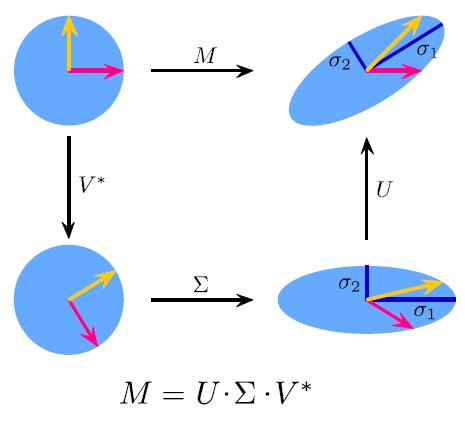
\includegraphics[width=4cm]{fig_1_3.jpg} 
    \caption{Illustration of SVD in $\mathbb{R}^2$}\label{fig_1_3}
\end{figure}
\par In the special case when $A$ is a real square matrix, i.e. $m=n$, $A$ can be interpreted as a linear transformation $\bm{x}\rightarrow A\bm{x}$ of $\mathbb{R}^m$. Orthogonal matrix $U$ and $V$ represent rotations or reflections and $\Sigma$ represents a scaling transform. Thus the SVD decomposition has a clear interpretation that it decompose any invertible linear transformation into a composition of a rotation or reflection ($V^T$), followed by a coordinate-wise scaling ($\Sigma$), followed by another rotation or reflection ($U$).
\begin{remark}
SVD can be computed in an iterative manner with time complexity $O(mn^2)$, assuming that $m\geq n$.
\end{remark}

\section{Continuation of Linear Autoencoder}
With the tool of SVD and Eckart Young Theorem (Theorem \ref{thm_1_EY}), we now can compute the optimal linear autoencoder. Define $U_k=[\bm{u}_1\bm{u}_2\dots \bm{u}_k]\in \mathbb{R}^{m\times k}$ as the first $k$ columns of $U$. We have the following proposition:
\begin{proposition}
$C^*=U_k^T$ and $D^*=U_k$ yields minimal reconstruction error for a linear autoencoder with k hidden units.
\end{proposition}
\begin{proof}
With $X=U\Sigma V^T\ s=\min\{m,n\}$ and $\hat{X}=DCX$ we have
\begin{equation*}
    \hat{X} = U_k U_k^T U\Sigma V^T = \left(\sum_{i=1}^{k}\bm{u}_i\bm{u}^T_i\right)\left(\sum_{i=1}^{s}\sigma_i\bm{u}_i\bm{v}^T_i\right) = \sum_{i=1}^{k}\sigma_i\bm{u}_i\bm{v}^T_i = U\Sigma_kV^T,
\end{equation*}\\
where the third equality follows $\bm{u}_i^T\bm{u}_j=\delta_{ij}$. By Theorem \ref{thm_1_EY}, $\hat{X}$ is optimal in terms of Frobenius norm as the reconstruction measure.
\end{proof}
\begin{remark}\label{rmk_1_1}
The optimal linear autoencoder via SVD is not the unique optimal solution, since for any invertible matrix $A\in\mathbb{R}^{k\times k}$, $C=AU_k^T$ and $D=U_kA^{-1}$ also give the optimal reconstruction error. This gives a particularly interesting insight into the interpretability of the features found by training a linear autoencoder. We can expect that there's randomness (some invertible $A$ introduced by randomness in our model) in the solution.
\end{remark}
A way to alleviate the problem of uniqueness mention in Remark \ref{rmk_1_1} is to do so called \emph{weight sharing}. Specifically, instead of optimizing over both $C$ and $D$, we require $D=C^T$. Note that this does not reduce the modeling power. Now the ambiguity in the optimal solution reduces to orthogonal group: 
\begin{equation*}
    A^{-1}=A^T,\ \text{i.e.}\ A\in O(k)
\end{equation*}
In another word, the mapping $\bm{x}\mapsto \bm{z}$ now is uniquely determined up to rotations (permutations, reflections). It's the same orthogonal subspace of the first k eigenvectors (different basis or axes).
%%%%%%%%%%%%%%%%%%%%%%%%%%%%%%%%%%%%%%%%%%%%%%%%%%%%%%%
%   New Chapter                                       %
%%%%%%%%%%%%%%%%%%%%%%%%%%%%%%%%%%%%%%%%%%%%%%%%%%%%%%%

\chapter{Principal Component Analysis}
In the last chapter, we discussed linear dimension reduction via linear autoencoder. Now we try to understand linear dimension reduction in a principled manner. We start with 1-dimension case, i.e. we want to approximate a group of points via points on a line. Then we generalize it to multiple dimensions, which yields exactly the idea of PCA. Finally we introduce a simple algorithm to find the dominant eigenvector of a matrix, followed by some examples and comparison with Linear Autoencoder we discussed in the last chapter.
\section{1D Linear Case}
\subsection{Line in $\mathbb{R}^m$}
Mathematically, we can represent a line in $\mathbb{R}^m$ in the following parametric form:
\begin{equation*}
    \bm{\mu} + \mathbb{R}\bm{u} \equiv \{\bm{v}\in \mathbb{R}^m:\exists z\in \mathbb{R}\ s.t.\ \bm{v}=\bm{\mu} + z\bm{u} \}
\end{equation*}
where $\bm{\mu}$ is the offset or shift, $\bm{u}$ is the direction vector such that $\|\bm{u}\|=1$. Note that representation is not unique since a scaling on $\bm{u}$ and a shifting on $\bm{\mu}$ along $\bm{u}$ will not change the line. 
\subsection{Approximation of a single point: orthogonal projection}
Now consider the task to approximate a data point $\bm{x}\in\mathbb{R}^m$ by a point on the line. It natural to request that our approximation should be close to the original point in Euclidean distance. Formally, we try to solve
\begin{equation}\label{eq_2_1}
    \mathop{\arg\min}_{z\in\mathbb{R}}\|\bm{\mu}+z\bm{u}-\bm{x}\|^2
\end{equation}
or equivalently,
\begin{equation*}
    \mathop{\arg\min}_{\hat{\bm{x}}\in \bm{\mu} + \mathbb{R}\bm{u}}\|\hat{\bm{x}}-\bm{x}\|^2
\end{equation*}
To solve (\ref{eq_2_1}), we request the first order optimality condition:
\begin{equation*}
    \frac{d}{dz}\|\bm{\mu}+z\bm{u}-\bm{x}\|^2 = 2\langle \bm{\mu}+z\bm{u}-\bm{x}, \bm{u}\rangle \overset{!}{=}0
\end{equation*}
this yields solutions
\begin{align*}
    z &= \langle \bm{x}-\bm{\mu},\bm{u} \rangle\\
    \hat{\bm{x}} &= \bm{\mu} + \langle \bm{x}-\bm{\mu},\bm{u} \rangle \bm{u}
\end{align*}
which is the \emph{orthogonal projection} of $\bm{x}$ to the line. 
\subsection{Optimal Line for multiple points}
Assume we are given data points $\{\bm{x}_1,\dots,\bm{x}_n\}\subset \mathbb{R}^m$. With the orthogonal projection result, the optimal approximation of $\{\bm{x}_i\}$ by a line $(\bm{u},\bm{\mu})$ is given by $\{\bm{\mu} + \langle \bm{x}_i-\bm{\mu},\bm{u} \rangle\}$. Therefore the optimal line can be found by solving
\begin{equation*}
    \mathop{\arg\min}_{(\bm{u},\bm{\mu})} \left[ \frac{1}{2n}\sum_{i=1}^n \| \bm{\mu}+ \langle \bm{x}_i-\bm{\mu},\bm{u\rangle\bm{u} - \bm{x}_i} \|^2\right]
\end{equation*}
using that $\langle\bm{v},\bm{u}\rangle\bm{u}=(\bm{u}\bm{u}^T)\bm{v}$, it's equivalent to
\begin{equation}\label{eq_2_obj}
    \mathop{\arg\min}_{(\bm{u},\bm{\mu})} \left[ \frac{1}{2n}\sum_{i=1}^n \left\| \left(I-\bm{u}\bm{u}^T \right)(\bm{x}_i-\bm{\mu}) \right\| ^2\right]
\end{equation}
Matrix $\left(I-\bm{u}\bm{u}^T \right)$ act as a linear map, more specifically, as a projection. Take an argument $\bm{v}$, by associativity, we get
\begin{equation*}
    \left(I-\bm{u}\bm{u}^T \right)\bm{v} = \bm{v} - \langle \bm{u}, \bm{v}\rangle\bm{u}
\end{equation*}
The RHS is the vector itself minus the projection to the line $\mathbb{R}\bm{u}$, which is the projection to the orthogonal complement $(\mathbb{R}\bm{u})^{\bot}$. Also, this projection is \emph{idempotent}, i.e. not changed in value following multiplication by itself, since
\begin{equation*}
     \left(I-\bm{u}\bm{u}^T \right)( \bm{v} - \langle \bm{u}, \bm{v}\rangle\bm{u}) =  \bm{v} - \langle \bm{u}, \bm{v}\rangle\bm{u} - ( \langle \bm{u}, \bm{v}\rangle\bm{u} -  \langle \bm{u}, \bm{v}\rangle\bm{u}) =  \bm{v} - \langle \bm{u}, \bm{v}\rangle\bm{u}
\end{equation*}
To solve (\ref{eq_2_obj}), we first request the first order optimality condition for $\bm{\mu}$
\begin{align*}
    &\nabla_{\bm{\mu}} \left[ \frac{1}{2n}\sum_{i=1}^n \left\| \left(I-\bm{u}\bm{u}^T \right)(\bm{x}_i-\bm{\mu}) \right\| ^2\right] \overset{!}{=} 0\\
    \Longleftrightarrow &  \frac{1}{n}\sum_{i=1}^n  \left(I-\bm{u}\bm{u}^T \right)(\bm{x}_i-\bm{\mu}) \overset{!}{=} 0\\
    \Longleftrightarrow & \left(I-\bm{u}\bm{u}^T \right)(\frac{1}{n}\sum_{i=1}^n\bm{x}_i-\bm{\mu})\overset{!}{=} 0
\end{align*}
Note that $\|\bm{u}\|=1$, then $\bm{u}$ is a eigenvector of $I-\bm{u}\bm{u}^T $ with corresponding eigenvalue 0. From this we see that the optimal solution of $\bm{\mu}$ is not unique. Any $\bm{\mu}$ satisfying 
\begin{equation*}
    \frac{1}{n}\sum_{i=1}^n\bm{x}_i-\bm{\mu} = k\bm{u},\ k\in \mathbb{R}
\end{equation*}
will be an optimal solution. We can also see this from another intuitive angle: any $\bm{\mu}$ lies on the optimal line should be a equivalent in terms of determining a line.
\par Despite the first order optimality condition cannot determine $\bm{\mu}$ uniquely, there is a unique solution for all $\bm{u}$:
\begin{equation*}
    \bm{\mu} = \frac{1}{n}\sum_{i=1}^n\bm{x}_i \equiv sample\ mean
\end{equation*}
which means that all the lines that are optimal in this 1-D setting have to pass through $ \bm{\mu} = \frac{1}{n}\sum_{i=1}^n\bm{x}_i$. Since it will be good to have a "correct" $\bm{\mu}$ that can guarantee optimality without the dependency on $\bm{u}$, we simply choose $\bm{\mu}$ to be the sample mean.
\par By choosing $\bm{\mu} = \frac{1}{n}\sum_{i=1}^n\bm{x}_i$, what we are doing is often referred to as \emph{centering} in the data in ML literature. By centering the data, i.e.
\begin{equation*}
    \bm{x}_i\leftarrow \bm{x}_i-\frac{1}{n}\sum_{i=1}^n\bm{x}_i
\end{equation*}
we identify the center of mass with the origin and restrict the problem to linear (instead of affine) subspaces. This will simplify the derivations and analyses without loss in modeling power. Therefore from now on, w.l.o.g. we assume that the data points are centered.
\par By centering the data, the optimization problem is left with
\begin{align}
    &\mathop{\arg\min}_{\|\bm{u}\|=1} \left[ \frac{1}{n}\sum_{i=1}^n \|\langle \bm{x}_i,\bm{u}\rangle \bm{u} - \bm{x}_i\|^2 \right]\notag\\
    \Longleftrightarrow &\mathop{\arg\min}_{\|\bm{u}\|=1} \left[ \frac{1}{n}\sum_{i=1}^n \|\langle \bm{x}_i,\bm{u}\rangle \bm{u}\|^2 + \|\bm{x}_i\|^2 - 2\langle \bm{x}_i,\bm{u}\rangle^2 \right]\notag\\
    \Longleftrightarrow &\mathop{\arg\min}_{\|\bm{u}\|=1} \left[- \frac{1}{n}\sum_{i=1}^n\langle \bm{x}_i,\bm{u}\rangle^2 \right]\ (\bm{x}_i\text{ is a const})\notag\\
    \Longleftrightarrow &\mathop{\arg\min}_{\|\bm{u}\|=1} \left[- \frac{1}{n}\sum_{i=1}^n\ \bm{u}^T\bm{x}_i\bm{x}_i^T\bm{u} \right]\notag\\
    \label{eq_2_obj_u}\Longleftrightarrow &\mathop{\arg\min}_{\|\bm{u}\|=1} \left[- \bm{u}^T\left(\frac{1}{n}\sum_{i=1}^n\ \bm{x}_i\bm{x}_i^T\right)\bm{u} \right]\ (\text{Associativity})
\end{align}
where the matrix between $\bm{u}^T$ and $\bm{u}$ is call \emph{variance-covariance matrix} of the data sample
\begin{equation*}
    \bm{\Sigma} \equiv \frac{1}{n}\sum_{i=1}^n\ \bm{x}_i\bm{x}_i^T = \frac{1}{n}{\bf XX}^T \in \mathbb{R}^{m\times m},\ {\bf X}\equiv[\bm{x}_1,\dots,\bm{x}_n]
\end{equation*}
This gives us a very important insight: in the 1-D setting, $\bm{u}$ depends on the data only through ${\bf \Sigma}$. This is remarkable, since the dependency between $\bm{u}$ and all the data points ${\bf X}$ can be very complicated and there are a lot of information in ${\bf X}$. But (\ref{eq_2_obj_u}) tells us the only thing matters is ${\bf \Sigma}$. Consider we want to fit the data in a streaming manner, the above analysis shows that we can update $\bm{u}$ very efficiently by recomputing ${\bf \Sigma}$.
\par Problem (\ref{eq_2_obj_u}) is a constrained optimization problem. To solve it we introduce the Lagrange multiplier $\lambda$ and define the following Lagrangian
\begin{equation}\label{eq_1_lag}
    L(\bm{u},\lambda) = -\bm{u}^T\bm{\Sigma u} + \lambda (\bm{u}^T\bm{u}-1)
\end{equation}
Before trying to solve it, we first take another view from the duality view and gain some insight into the Lagrange method. Assume we have a primal player who wants to minimize the objective in (\ref{eq_2_obj_u}). To remove the constraint on $\bm{u}$, we introduce a dual player who wants to maximize the objective and would exploit a deviation from the original constraint on $\bm{u}$. Formally, we consider
\begin{equation}\label{eq_2_dual}
    \min_{\bm{u}}\max_{\lambda} -\bm{u}^T\bm{\Sigma u} + \lambda (\bm{u}^T\bm{u}-1)
\end{equation}
If the primal player (picking $\bm{u}$ and attempting to minimize the objective) picks $\bm{u}$ that does not satisfy the original constraint, the dual player (picking $\lambda$ and trying to maximizing the objective) will be able to drive the objective value to $+\infty$ since there's no constraint on $\lambda$. Then is clear that (\ref{eq_2_dual}) is equivalent to (\ref{eq_2_obj_u}).
\par With this intuition, we now try to solve (\ref{eq_1_lag}) by again applying the first order optimality condition:
\begin{equation*}
    \nabla_{\bm{u}} L(\bm{u},\lambda) = -2(\bm{\Sigma u}-\lambda \bm{u})\overset{!}{=}0 \Longleftrightarrow \bm{\Sigma u}=\lambda \bm{u}
\end{equation*}
This means that minimizing over $\bm{u}$ requires $\bm{u}$ to be an eigenvector of ${\bf \Sigma}$ with the corresponding eigenvalue $\lambda$. Since we want to maximize over $\lambda$, $\bm{u}$ should be a \textbf{principal} eigenvector of $\bm{\Sigma}$. So the optimal direction of the line is the principal eigenvector of the sample variance-covariance matrix. Also we have the following extremal characterization
\begin{equation*}
    \bm{u} = \mathbb{\arg\max}_{\bm{v}:\|\bm{v}\|=1}\left[\bm{v}^T\bm{\Sigma v} \right]
\end{equation*}
\begin{remark}\label{rmk_2_1}
Usually, even we can mathematically define and find the eigenvectors and eigenvalues of a matrix, it is still hard to interpret what these vectors and values are. The discussion above give us some insight of the principal eigenvector (of a variance-covariance matrix of centered data) in terms of 1-D PCA. It is the direction that the projected data have the smallest reconstruction error and also the direction of largest data variance (we will see this soon).
\end{remark}
\par Before we finish this section, we re-interpret the 1-D PCA problem, as suggested in the end of Remark (\ref{rmk_2_1}), in terms of variance maximization in 1-D representation. 
\par Consider the variance of the projected data (remember that we assume centered data, which means the projections (a linear transformation) will also be centered)
\begin{equation*}
    \text{Var}[z]=\frac{1}{n}\sum_{i=1}^{n}z_i^2=\frac{1}{n}\sum_{i=1}^{n}\langle \bm{x}_i,\bm{u}\rangle^2 = \bm{u}^T\bm{\Sigma u}
\end{equation*}
This shows the equivalence of
\begin{itemize}
    \item Direction of the smallest reconstruction error.
    \item Direction of the largest data variance.
\end{itemize}
\section{Principal Component Analysis}
Define the residual as the projection of the data to $(\mathbb{R}\bm{u})^{\bot}$:
\begin{equation*}
    \bm{r}_i:=\bm{x}_i - \langle\bm{x}_i,\bm{u}  \rangle\bm{u} = \left({\bf I} - \bm{uu}^T \right)\bm{x}_i
\end{equation*}
The variance-covariance matrix of the residual vectors is
\begin{align*}
    \frac{1}{n}\sum_{i=1}^n \bm{r}_i\bm{r}_i^T &=  \frac{1}{n}\sum_{i=1}^n \left({\bf I} - \bm{uu}^T \right)\bm{x}_i\bm{x}_i^T\left({\bf I} - \bm{uu}^T \right)\\
    &= \left({\bf I} - \bm{uu}^T \right)\bm{\Sigma}\left({\bf I} - \bm{uu}^T \right)\\
    &=\bm{\Sigma} - \lambda\bm{uu}^T\ (\bm{\Sigma u}=\lambda \bm{u},\ \bm{u}^T\bm{u}=1)
\end{align*}
This matrix has some interesting properties. First, $\bm{u}$ is its eigenvector with eigenvalue $0$:
\begin{equation*}
    \left(\bm{\Sigma} - \lambda\bm{uu}^T\right)\bm{u} = \bm{\Sigma u}-\lambda \bm{u}=0
\end{equation*}
Recall the eigen-decomposition of $\bm{\Sigma}$
\begin{equation}\label{eq_2_edom}
    \bm{\Sigma} = \sum_{i=1}^m \lambda_i\bm{u}_i\bm{u}_i^T
\end{equation}
where $\lambda_1\geq\dots\geq\lambda_m\geq 0$ are the eigenvalues of $\Sigma$ (the non-negativity is from that $\Sigma$ is positive semi-definite (p.s.d.)) and $\bm{u}_i$'s are corresponding eigenvectors. Also we have $\lambda = \lambda_1$ and $\bm{u}=\bm{u}_1$ by the discussion so far. Therefore, we obtain
\begin{equation*}
    \bm{\Sigma} - \lambda\bm{uu}^T = \sum_{i=1}^m \lambda_i\bm{u}_i\bm{u}_i^T - \lambda_1\bm{u}_1\bm{u}_1^T = \sum_{i=2}^m \lambda_i\bm{u}_i\bm{u}_i^T
\end{equation*}
which suggests that the eigenvectors of $\bm{\Sigma} - \lambda\bm{uu}^T$ are still the eigenvectors of $\bm{\Sigma}$, so are the eigenvalues expect that the eigenvalue of $\bm{u}_1$ changes to $0$. This means that the principal eigenvector of $\bm{\Sigma} - \lambda\bm{uu}^T$ is the second principal eigenvector of $\bm{\Sigma}$. Moreover, the second principal eigenvector of $\bm{\Sigma}$ is the direction that has the smallest reconstruction error as well as the largest variance over the residual data.
\par Repeating the above procedure, i.e. finding the principal eigenvector of $\bm{\Sigma}-\lambda \bm{uu}^T$, which is the 2nd principal eigenvector of $\bm{\Sigma}$, we can iteratively identity the $d$ principal eigenvectors of $\bm{\Sigma}$. Note that the eigenvectors are guaranteed to be pairwise orthogonal.
\par Let us take a matrix view to complement the iterative one. The eigen-decomposition (\ref{eq_2_edom}) can also be written in a matrix form (also known as diagonalization):
\begin{equation*}
    {\bf \Sigma = U\Lambda U}^T,\ {\bf \Lambda} =\text{diag}(\lambda_1,\dots, \lambda_m),\ \lambda_1\geq\dots\geq\lambda_m\geq 0
\end{equation*}
where ${\bf U}$ is an orthogonal matrix (unit length, orthogonal columns) with its columns are eigenvectors of $\bm{\Sigma}$ (form an eigenvector basis):
\begin{equation*}
    {\bf U}=(\bm{u}_1,\dots,\bm{u}_m),\ {\bf U}^T\bm{u}_i=\bm{e}_i,\ \bm{\Sigma u}_i = \lambda_i\bm{u}_i
\end{equation*}
The following are 2 useful results from linear algebra
\begin{theorem}\label{thm_2_spectral}
(Spectral Theorem): Matrix ${\bf A}$ is diagonalizable by an orthogonal matrix if and only if it is symmetric.
\end{theorem}
\begin{theorem}
Distinct eigenvalues of symmetric matrices have orthogonal eigenvectors.
\end{theorem}
\begin{proof}
\begin{equation*}
    \lambda_j \bm{u}_i^T\bm{u}_j = \bm{u}_i^T{\bf A}\bm{u}_j = \bm{u}_j^T{\bf A}\bm{u}_i = \lambda_i \bm{u}_j^T\bm{u}_i
\end{equation*}
Since $\lambda_i\neq \lambda_j$, we have $\bm{u}_i^T\bm{u}_j=0$.
\end{proof}
\vbox{}
\par Note that $\bm{\Sigma}=\frac{1}{n}{\bf XX^T}$ is symmetric, with the above 2 theorems, the optimal reduction to $d$ dimension via PCA is to compute the first d coordinates of the data in the basis formed by eigenvectors of $\bm{\Sigma}$:
\begin{equation*}
    {\bf Z}={\bf \tilde{U}}^T{\bf X}\in \mathbb{R}^{d\times n},\ {\bf \tilde{U}} = (\bm{u}_1,\dots,\bm{u}_d)\in\mathbb{R}^{m\times d},\ d\leq m
\end{equation*}
and the optimal reconstruction (guaranteed by Eckart-Young (Theorem \ref{thm_1_EY})) is to project the data to the spanning subspace of the $d$ principal eigenvectors of $\bm{\Sigma}$:
\begin{equation*}
    {\bf \tilde{X}}={\bf \tilde{U}Z} = {\bf \tilde{U}\tilde{U}}^T{\bf X}
\end{equation*}
where ${\bf \tilde{U}\tilde{U}}^T$ is the projection matrix.
\section{Algorithms and Interpretation}
\subsection{Power Method}
Eigenvalues and eigenvectors are extremely important for analytic purposes. Sometimes we want to know exactly what the eigenvectors and the eigenvalues is, which call for development of efficient algorithm to compute them. Power iteration is a simple algorithm for finding dominant eigenvector of ${\bf A}$.
\par As is suggested by its name, power iteration is done in a iterative way. We start from a random vector $\bm{v}_0$, multiply by ${\bf A}$, normalize it and do it all over again
\begin{equation*}
    \bm{v}_{t+1} = \frac{{\bf A}\bm{v}_t}{\|{\bf A}\bm{v}_t\|}
\end{equation*}
where we made two technical assumptions:
\begin{equation}\label{eq_2_asp}
    \langle \bm{u}_1,\bm{v}_0\rangle\neq 0\ \text{and}\ |\lambda_1|>|\lambda_j|(\forall j\geq2)
\end{equation}
Note that if we pick $\bm{v}_0$ uniformly random, the first assumption is satisfied with probability 1. The following proposition shows the convergence of Power Iteration for p.s.d. and symmetric ${\bf A}$ when the two assumptions are satisfied.
\begin{proposition}
For Power Iteration algorithm we discussed above, if $\bm{v}_0$ and ${\bf A}$ satisfy (\ref{eq_2_asp}) then it follows
\begin{equation*}
    \lim_{t\rightarrow\infty}\bm{v}_t=\bm{u}_1
\end{equation*}
and we can also recover $\lambda_1$ from Rayleigh quotient:
\begin{equation*}
    \lambda_1 = \lim_{t\rightarrow \infty} \frac{\|{\bf A}\bm{v}_t\|}{\|\bm{v}_t\|}
\end{equation*}
\end{proposition}
\begin{proof}
Since ${\bf A}$ is p.s.d. and symmetric, by Spectral Theorem (Theorem \ref{thm_2_spectral}) we know it is diagonalizable, and therefore has eigenbasis $\{\bm{u}_1,\dots,\bm{u}_m\}$. We can write $\bm{v}_0$ as a linear combination of $\{\bm{u}_1,\dots,\bm{u}_m\}$:
\begin{equation*}
    \bm{v}_0 = \sum_{i=1}^{m} \alpha_i \bm{u}_i,\ \alpha\neq0
\end{equation*}
With the eigen-decomposition of ${\bf A}$: ${\bf A}= \sum_{i=1}^m \lambda_i\bm{u}_i\bm{u}_i^T $ and using that fact that $\bm{u}_i$'s are orthogonal, we have for any vector $\bm{v} = \sum_{i=1}^{m} w_i \bm{u}_i$
\begin{equation*}
    {\bf A}\bm{v} = (\sum_{i=1}^m \lambda_i\bm{u}_i\bm{u}_i^T)(\sum_{i=1}^{m} w_i \bm{u}_i) = \sum_{i=1}^{m} \lambda_i w_i \bm{u}_i
\end{equation*}
which shows that multiplying a vector by ${\bf A}$ is equivalent to multiplying $\lambda_i$'s to each corresponding coordinate under basis $\{\bm{u}_1,\dots,\bm{u}_m\}$. Note that even if we do normalization in each time step (for numerical reason), it will not affect the direction of ${\bf A}\bm{v}_t$ and therefore is equivalent to normalize just once at the end. Thus, denote the normalization factor in the last step as $c_t$ we obtain
\begin{equation*}
    \lim_{t\rightarrow \infty}\bm{v}_t = \lim_{t\rightarrow \infty}\frac{1}{c_t}\sum_{i=1}^{m} \lambda_i^t \alpha_i \bm{u}_i = \lim_{t\rightarrow \infty}\frac{\lambda_1^t\alpha_1}{c_t} \left(\bm{u}_1 + \sum_{i=2}^{m} \frac{\alpha_i}{\alpha_1}\left(\frac{\lambda_i}{\lambda_1}\right)^t\bm{u}_i\right) = \bm{u}_1
\end{equation*}
as $\lambda_j<\lambda_1$. Note that $c_t$ is a normalization factor, thus $c_t\rightarrow 1/(\lambda_1^t\alpha_1)$.
\end{proof}
\subsection{Example}
Digital images are saved in matrix which can be vectorized and we can then apply PCA to analyze digital images. The following is the mean vector and first four principal directions (with eigenvalues) of number three in a digital number data set. (the blue means positive and yellow means negative)
\begin{figure}[h]
    \centering 
    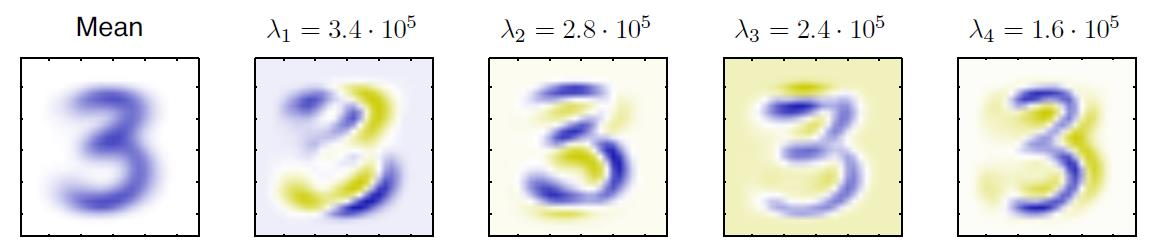
\includegraphics[width=10cm]{fig_2_1.jpg} 
    \caption{Digital number example of PCA}\label{fig_2_1}
\end{figure}
\begin{figure}[h] 
    \centering 
    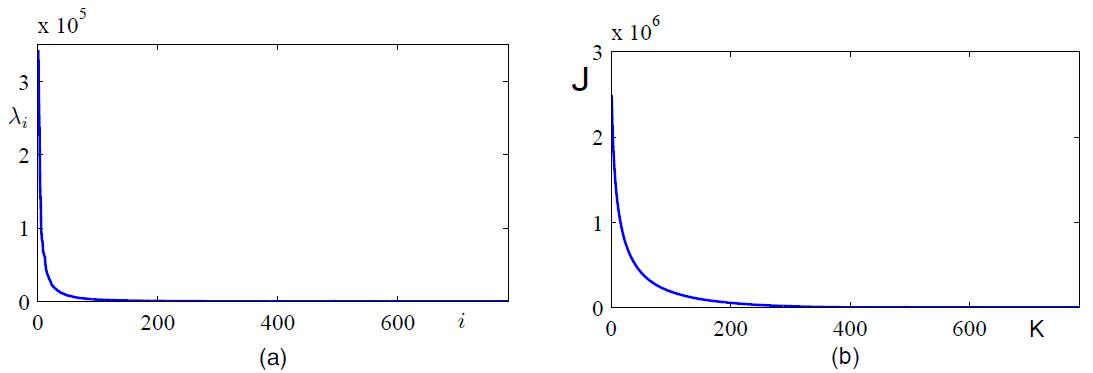
\includegraphics[width=10cm]{fig_2_2.jpg} 
    \caption{Eigenvalue spectrum example (left), and approximation error (right)}\label{fig_2_2}
\end{figure}
\par We can see that (Figure \ref{fig_2_1}) the first 4 principal eigenvectors have very clear interpretation. The first one mainly deals with tilting, and the 4th one probably handles scaling. Also the eigenvalues show the importance of each principal vector.
\par It's also very helpful to look at the eigenvalue spectrum (Figure \ref{fig_2_2}). For structured data like natural images, there is usually a fast decay in its eigenvalue spectrum. Since the reconstruction error depends on the sum of eigenvalues we ignore, there is usually a fast decay in reconstruction loss w.r.t. the number of principal components.
\par In the discussion so far, we always assume that the number of principal components (also for the reduced dimension number in Linear Autoencoder) is predefined and fixed. A natural question to ask is how should we choose this number, which is sometimes called \emph{intrinsic dimensionality} . A heuristic strategy is to look at the spectrum of eigenvalues and detect the "knee" or "elbow". However, in practice, there are usually more things like the limit of computational power or storage that determine how we choose the number of reduced dimensions.
\begin{figure}[h] 
    \centering 
    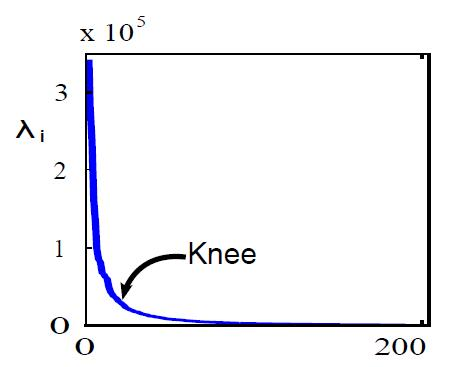
\includegraphics[width=6cm]{fig_2_3.jpg} 
    \caption{Detect "knee" to determine intrinsic dimensionality}\label{fig_2_3}
\end{figure}
\subsection{Comparison with Linear Autoencoder Network}
At this point, it is worth spending some time comparing the two dimension reduction method we learned:
\begin{itemize}
    \item PCA clarifies that one should (ideally) center the data, while it's not explicit in Linear Autoencoder.
    \item PCA representation is unique (if no eigenvalue multiplicities) and as such (in principle) interpretable.
    \item Linear autoencoder without weight sharing is highly non-interpretable (lack of identifiability).
    \item Linear autoencoder with weight sharing: ${\bf C=D^T}$ identifies the same subspace of $k$ principal eigenvectors (see discussion after Remark \ref{rmk_1_1}), but axes are non-identifiable. To modify an autoencoder to identify the principal axes, techniques like adding regularization to enforce ordering in the axis can be applied.
    \item General lesson for neural networks based method: caution with naively interpreting learned (neural) representations.
\end{itemize}
\par For the algorithm used to find the solution:
\begin{itemize}
    \item Compute one principal component at a time via power iterations: good for small $k$, conceptually easy and robust.
    \item Train a linear auto encoder via backpropagation: it's easily extensible and we use stochastic optimization (stochastic gradient descent), which is good for very large data set and has good convergence properties.
    \item Compute PCA from SVD: good for mid-sized problems, can leverage wealth of numerical techniques for SVD (e.g. QR decomposition)
\end{itemize}
\subsection{PCA via SVD}
The power iteration algorithm and eigen-decompostion, which has time complexity $O(m^3)$ for $\bm{\Sigma}\in\mathbb{R}^{m\times m}$, suffer from large $m$. A way to solve the problem for the case that $m$ is considerably large compared with $n$ is to use SVD, which only takes $O(mn^2)$ for ${\bf X}\in \mathbb{R}^{m\times n}$.
\par To compute the eigen-decomposition of ${\bf AA}^T$ via SVD:
\begin{equation*}
    {\bf AA}^T = ({\bf UDV})({\bf VD}^T{\bf U}^T) = {\bf UDI_nD}^T{\bf U}^T = {\bf U\Lambda U}^T
\end{equation*}
where ${\bf \Lambda} = {\bf DD}^T=\text{diag}(\lambda_1,\dots,\lambda_m)\in\mathbb{R}^{m\times m}$ and
\begin{equation*}
\lambda_i=\begin{cases}
\sigma_i^2& \text{for }1\leq i \leq \min\{n,m\}\\
0& \text{for }n< i \leq m
\end{cases}
\end{equation*}
Similarly we have ${\bf A}^T{\bf A}={\bf V\Lambda'V}^T$, where
\begin{equation*}
    {\bf \Lambda'} = {\bf D}^T{\bf D} = \text{diag}(\lambda'_1,\dots,\lambda'_n)\in\mathbb{R}^{n\times n},\ \lambda'_i=\begin{cases}
\lambda_i^2& \text{for }1\leq i \leq \min\{n,m\}\\
0& \text{for }m< i \leq n
\end{cases}
\end{equation*}
We see that ${\bf U}$, i.e. the left singular vectors of A, is the eigenvectors of ${\bf AA}^T$, and ${\bf V}$, i.e. the right singular vectors of A, is the eigenvectors of ${\bf A}^T{\bf A}$. ${\bf \Lambda}$ and ${\bf \Lambda}$ are identical up to zero padding. This shows that we can used the SVD of ${\bf X}$ to compute the eigen-decomposition of ${\bf \Sigma}=\frac{1}{n}{\bf XX}^T$. But when $n \gg m$, SVD is not so competitive. Also note that, eigen-decomposition of ${\bf \Sigma}$ suffers from very large and small $\sigma_i$'s in terms of numerical stability since it involves squares compared with using the SVD.
%%%%%%%%%%%%%%%%%%%%%%%%%%%%%%%%%%%%%%%%%%%%%%%%%%%%%%%
%   New Chapter                                       %
%%%%%%%%%%%%%%%%%%%%%%%%%%%%%%%%%%%%%%%%%%%%%%%%%%%%%%%

\chapter{Matrix Approximation and Reconstruction}
In chapter 1, we discussed about low-rank matrix approximation, while in this chapter we will introduce a slightly different topic, Matrix Completion, which is the task of filling in the missing entries of a partially observed matrix. The matrix completion problem is in general NP-hard, but we will show in this chapter that under the low-rank assumption there are algorithms that can do exact reconstruction with high probability. We will start by introducing the famous Netflix problem and collaborative filtering, of which matrix completion is at the heart.
\section{Collaborative Filtering}
Collaborative filtering is a classical example of matrix completion and is a technique that is frequently used in recommender systems. Given the entire data set, a recommender system needs to analyze patterns of interest in terms (products, movies, ...) and provide personalized recommendations for users. With the motivation that every user has a relative stable preference and similar users have similar preferences, collaborative filtering exploits collective data from many users and builds models that can generalize across users and , possibly also, across items.
\par Consider the Netflix Data, which is a matrix with its rows correspond to users and columns refer to different movies. Each entry of this matrix is a 1-5 star rating of a movie given by a user, while, of course, there are a lot of missing values. Also, the data is imbalanced in a way that there are users gave a lot of ratings while some did not, so as the movies. The task is to predict the missing values. In another word, to complete the matrix.
\par Let the size of the rating matrix to be  $m\times n$. One way to complete the matrix is to build a statistical model with $k\ll m\times n$ parameters that introduces coupling between entries and then infer the missing entries from the observed ones. This can be formalized in a low-rank decomposition manner: we want to find the best approximation with low rank $r\ll \min\{m,n\}$. In this case, number of the parameters $k$, i.e. the number of entries in decomposition, satisfies $k\leq r\cdot (m+n)\ll m\times n$.
\section{Matrix Approximation via SVD}
We first briefly review some of the concepts from linear algebra, which are helpful and necessary for understanding the matrix approximation method via SVD. We start by revisiting 2 frequently used matrix norms.
\begin{definition}
	(Frobenius norm) For a matrix ${\bf A}\in \mathbb{R}^{m \times n}$, its Frobenius is given by
	\begin{equation*}
		\|{\bf A}\|_F :=\sqrt{\sum_{i=1}^{m}\sum_{j=1}^{n}a_{ij}^2}=\|vec({\bf A})\|_2=\sqrt{trace({\bf A}^T{\bf A})}
	\end{equation*}
\end{definition}
Frobenius norm only depends on the singular values of ${\bf A}$:
\begin{equation*}
	\|{\bf A}\|_F^2 = \sum_{i=1}^{k}\sigma_i^2,\ k=\min\{m,n\}
\end{equation*}
which follows from the cyclic property of trace: $trace({\bf ABC})=trace({\bf BCA})$:
\begin{equation*}
	trace({\bf A}^T{\bf A}) = trace({\bf VD}^T{\bf U}^T{\bf UDV}^T)=trace({\bf V}^T{\bf VD}^T{\bf D}) = \sum_{i=1}^{k}\sigma_i^2
\end{equation*}
\begin{definition}
	(Induced $p$-norm) For a matrix ${\bf A}\in \mathbb{R}^{m \times n}$, its induced $p$-norm is given by
	\begin{equation*}
	\|{\bf A}\|_p :=\sup\{\|{\bf A}\bm{x}\|_p:\ \|\bm{x}\|_p=1\},\ \|\bm{x}\|_p:=\left(\sum_{i}|x_i|^p\right)^{1/p}
	\end{equation*}
\end{definition}
where for $p=2$ it's also called \emph{spectral norm}, which is equal to the largest singular value
\begin{definition}
	(Spectral norm) For a matrix ${\bf A}\in \mathbb{R}^{m \times n}$, its spectral norm is given by
	\begin{equation*}
	\|{\bf A}\|_2 :=\sup\{\|{\bf A}\bm{x}\|_2:\ \|\bm{x}\|_2=1\}=\sigma_1({\bf A})
	\end{equation*}
\end{definition}
The statement that the spectral norm is equal to the largest singular value follows from
\begin{align*}
	\|{\bf A}\bm{x}\|_2^2 
	&= \bm{x}^T{\bf A}^T{\bf A}\bm{x}\\
	&=  \bm{x}^T{\bf VD}^T{\bf U}^T{\bf UDV}^T\bm{x}\\
	&= \bm{v}^T{\bf D}^2\bm{v}\ (\bm{v} = {\bf V}\bm{x}^T,\ \|\bm{v}\|_2=1)\\
	&= \sum_{i=1}^{k} \sigma_i^2v_i^2\leq \sigma_1^2\sum_{i=1}^{k}v_i^2 = \sigma_1^2
\end{align*}
where the inequality is met with equality when $\bm{v} = (1,0,\dots,0)$.
\par Finally, recall that Eckart-Young Theorem (Theorem \ref{thm_1_EY}) give the optimal low rank approximation in both Frobenius norm and spectral norm (see the proof of Theorem \ref{thm_1_EY}). Specifically, given ${\bf A}={\bf UDV}^T$, define for $k\leq rank({\bf A})$:
\begin{equation*}
	{\bf A}_k :=\sum_{i=1}^{k}\sigma_i \bm{u}_i\bm{v}_i^T,\ rank({\bf A}_k)=k
\end{equation*}
then ${\bf A}_k$ is the best approximation in terms of Frobenius norm and spectral norm:
\begin{align*}
	&\min_{rank({\bf B})=k}\|{\bf A}-{\bf B}\|^2_F=\|{\bf A}-{\bf A}_k\|_F^2=\sum_{r=k+1}^{rank({\bf A})} \sigma_r^2\\
	&\min_{rank({\bf B})=k}\|{\bf A}-{\bf B}\|_2=\|{\bf A}-{\bf A}_k\|_2=\sigma_{k+1}
\end{align*}
\section{SVD for Collaborative Filtering}
Assume that we have a fully observed rating matrix ${\bf A}$, then the SVD of ${\bf A}$ has a clear interpretation:
\begin{itemize}
	\item The truncated number of dimension $k$: number of latent factors.
	\item ${\bf U}$: user-to-factor association matrix.
	\item ${\bf V}$: items-to-factor association matrix.
	\item ${\bf D}$: level of strength (importance) of each factor.
\end{itemize} 
In the slide of matrix reconstruction, there is a very nice example to illustrate this interpretation of SVD.
\section{Algorithms for matrix completion}\label{sec_3_alg_for_mc}
\subsection{The hardness of matrix completion}
As we have mentioned at the beginning of the last section, the SVD solution of matrix reconstruction, suggested by Eckart-Young Theorem, requires fully observed rating matrices which in most of the times is not that case. The existence of unobserved entries turns the optimization problem from
\begin{equation}\label{eq_3_opt_full}
	\min_{rank({\bf B})=k}\left[\sum_{i,j}(a_{ij}-b{ij})^2 \right]=	\min_{rank({\bf B})=k}\|{\bf A}-{\bf B}\|_F^2
\end{equation} 
to
\begin{equation}\label{eq_3_opt_partial}
\min_{rank({\bf B})=k}\left[\sum_{(i,j)\in \mathcal{I}}(a_{ij}-b{ij})^2 \right],\ \mathcal{I}=\{(i,j):\ \text{observed}\}
\end{equation} 
where in both case we usually preprocess the data to have 
$$a_{ij}\leftarrow a_{ij}-\frac{1}{|\mathcal{I}|}\sum_{\mathcal{I}}a_{ij}$$
\par A natural attempt to remedy the problem is by replacing the unobserved entries by something like mean or zero, which is known as \emph{data imputation}. However, this attempt will fail miserably when there are a large number of missing values. 
\par Note that, even if Eckart-Young Theorem gives the optimal solution of (\ref{eq_3_opt_full}) miraculously, surprisingly the optimizing problem itself is not convex, since the rank constraint is not convex. It's not difficult to see this by noticing that the convex combination of rank 1 matrices may not give a rank 1 matrix:
\begin{equation*}
	\begin{gathered}
		\frac{1}{2}\begin{bmatrix}
		1 & 0 \\ 0 & 0
		\end{bmatrix} + 
		\frac{1}{2}\begin{bmatrix}
		0 & 0 \\ 0 & 1
		\end{bmatrix} =
		\frac{1}{2}\begin{bmatrix}
		1 & 0 \\ 0 & 1
		\end{bmatrix}
	\end{gathered}
\end{equation*}
\par The hardness of matrix completion can be seen from replacing the Frobenius norm in (\ref{eq_3_opt_full}) to weighted Frobenius norm defined as follow
\begin{definition}\label{def_3_wtd_f_norm}
	(Weighted Frobenius norm) the weighted Frobenius norm with regard to matrix ${\bf G}\geq {\bf 0}$ is defined as
	\begin{equation*}
	\|{\bf X}\|_{{\bf G}}:=\sqrt{\sum_{i,j}g_{ij}x_{ij}^2}
	\end{equation*}
\end{definition}
Note that the observation indicator matrix $\mathcal{I}$ is a special case of ${\bf G}$ for $g_{ij}\in\{0,1\}$ (Boolean).
\par It's known that in general, solving the following low-rank approximation problem is intrinsically hard
\begin{equation*}
	\min_{rank({\bf B})\leq k} \|{\bf A}-{\bf B}\|_{{\bf G}}^2
\end{equation*}
This is shown to be NP-hard (Gillis \& Glineur, 2011) even for $k=1$. The hardness also holds for approximations with prescribed accuracy and for binary ${\bf G}$.
\par So far we have seen that, matrix completion is a non-convex problem, which contributes a lot to its hardness. In general, the non-convexity of a problem comes from two aspects. 
\par The first one is the non-convex domain, as in the matrix completion with rank constraint (\ref{eq_3_opt_full}), where we minimize a convex objective over domain $\mathcal{Q}_k:=\{{\bf B}:rank({\bf B})=k\}$. The way to tackle it is really at the heart of \textbf{convex relaxation} that we are going to introduce, where we relax the non-convex constraint to have a convex domain.
\par The other one is the non-convex objective. In our matrix completion task, to remedy the non-convex rank constraint, we force this it by re-parameterizing ${\bf B}={\bf UV},\ {\bf U}\in \mathbb{R}^{m\times k},\ {\bf V}\in \mathbb{R}^{k\times n}$ since by definition $rank({\bf B})\leq k$. However, there is no free lunch, by doing reparametrization, the objective becomes non-convex. Consider $f(u, v) = (a-uv)^2$, which is a simplified case for matrix problem. For $a\neq 0$, there exists $u_1v_1=u_2v_2=a \land u_1\neq u_2$ that follows
\begin{equation*}
	f(u_1,v_1)=f(u_2,v_2)=0\land f(\frac{u_1+u_2}{2},\frac{v_1+v_2}{2})>0.
\end{equation*}
Despite the non-convexity of the new objective, it has some nice properties that lead to the \textbf{alternating least squares} method.
\begin{remark}
	An interesting thing to mention is that the decomposition ${\bf B} = {\bf UV}$ not only removes the non-convex rank constraint but also maintains a analogous interpretation as SVD. ${\bf U}$ captures user-to-factor association while ${\bf V}$ describes item-to-factor collaboration.
\end{remark}
\subsection{Alternating Least Squares}
Using the reparametrization, we make the domain convex, but at the same time, the objective function $f({\bf U}, {\bf V})$ is not jointly convex in ${\bf U}$ and ${\bf V}$. 
\begin{equation*}
	f({\bf U}, {\bf V})=\frac{1}{|\mathcal{I}|}\sum_{(i,j)\in \mathcal{I}}(a_{ij}-\langle\bm{u}_i,\bm{v}_j\rangle)^2
\end{equation*}
where $\bm{u}_i$'s are rows of ${\bf U}$ and $\bm{v}_i$'s are columns of ${\bf V}$. However, for fixed ${\bf U}$, $f$ is convex in ${\bf V}$. For fixed ${\bf V}$ in turn, $f$ is convex in ${\bf U}$. This observation suggests an alternating minimization over ${\bf U}$ and ${\bf V}$:
\begin{align*}
	&{\bf U}\leftarrow \mathop{\arg\min}_{{\bf U}} f({\bf U}, {\bf V})\\
	&{\bf V}\leftarrow \mathop{\arg\min}_{{\bf V}} f({\bf U}, {\bf V}),\quad \text{repeat until convergence}
\end{align*}
Since $f$ is never increased in this alternating minimization progress, and by definition (sum of squares) f is lower bounded by $0$, by monotone convergence theorem $f$ will converge as the number of iteration goes to infinity. However, the convergence of $f$ does not necessarily mean that ${\bf U}$ and ${\bf V}$ will also converge (say if they are not uniquely identifiable), and optimization may stuck at local optima.
\par This alternating minimization for low-rank matrix factorization is called \emph{alternating least squares} (ALS). Despite the drawbacks mentioned above, alternating least squares is very efficiently solvable. The fact that in each iteration we are dealing with a convex problem takes part of the reason. More importantly, ALS decompose $f$ into subproblems (convex), each of which can be solved independently. 
\par Consider ${\bf U}$ is fixed, then $f$ is decomposed into subproblems for columns of ${\bf V}$:
\begin{equation*}
		f({\bf U}, {\bf V})= \sum_{j}\left[\sum_{i:(i,j)\in \mathcal{I}} (a_{ij} - \langle \bm{u}_i,\bm{v}_j \rangle)^2\right] = \sum_{j} f_j({\bf U}, \bm{v}_j)
\end{equation*}
where $f_j({\bf U}, \bm{v}_j)$'s are independently solvable least square problems for columns $\bm{v}_j$'s of ${\bf V}$. By symmetry, this also holds for fixing ${\bf V}$ and optimizing ${\bf U}$. Note that columns of ${\bf V}$ ($\bm{v}_j \in \mathbb{R}^k$) are representations for each item, while rows of ${\bf U}$ ($\bm{u}_i \in \mathbb{R}^k$) are representations for each user. 
\par Typically, we favor solutions (${\bf U,V}$) with small Frobenius norm. So we add (squared) Frobenius norm regularizer to regularize matrix factor ${\bf U,V}$:
\begin{equation*}
	\Omega({\bf U,V})=\|{\bf U}\|_F^2 + \|{\bf V}\|_F^2
\end{equation*}
then we optimize a regularized problem
\begin{equation*}
	\min_{{\bf U,V}} \left(f({\bf U,V})+\mu\Omega({\bf U,V})\right),\ \text{for some }\mu>0
\end{equation*}
Since the (squared) Frobenius norm also decomposes, adding regularization does not change the separability structure of the problem.
\par In a word, what ALS for collaborative filtering is doing is to alternatively do the following:
\begin{itemize}
	\item Given low-dimensional representations for items (${\bf V}$ fixed), compute for each user independently the best representation, i.e. optimize rows of ${\bf U}$.
	\item Given low-dimensional representations for users (${\bf U}$ fixed), compute for each item independently the best representation, i.e. optimize columns of ${\bf V}$.
\end{itemize}
All optimization problems are least-square problems of small dimension ($\bm{u}_i,\bm{v}_j\in \mathbb{R}^k$).

\subsection{Convex Relaxation}
In this section, we exploit the other direction for solving the original non-convex optimization problem. We start by introducing another useful matrix norm, the nuclear norm.
\begin{definition}
	(Nuclear norm) The nuclear norm of a matrix ${\bf A}$ is defined as the sum of its singular values
	\begin{equation*}
		\|{\bf A}\|_*=\sum_{i}\sigma_i,\quad \sigma_i:\text{ singular values of }{\bf A}
	\end{equation*}
\end{definition}
Recall the definition of Frobenius norm $\|{\bf A}\|_F=\sqrt{\sum_{i}\sigma_i^2}$, then if we define $\bm{\sigma}({\bf A})=(\sigma_1,\dots,\sigma_n)$, we have
\begin{equation*}
	\|{\bf A}\|_F = \|\bm{\sigma}({\bf A})\|_2,\ \|{\bf A}\|_*=\|\bm{\sigma}({\bf A})\|_1
\end{equation*}
For a diagonal matrix ${\bf D}$, $\|{\bf D}\|_*=\text{Tr}({\bf D})$. For matrix ${\bf A}\in\mathbb{R}^{m\times n}$ of rank $r$, the following two inequalities describe the relation between the matrix norms we have met so far:
\begin{align*}
	&\|{\bf A}\|_2\leq \|{\bf A}\|_F\leq \sqrt{r}\|{\bf A}\|_2\\
	&\|{\bf A}\|_F\leq \|{\bf A}\|_*\leq \sqrt{r}\|{\bf A}\|_F
\end{align*} 
With the nuclear norm, what people usually look at in matrix reconstruction are the following 2 types of problems. The first one is exact reconstruction (given observed entries indicated by Boolean matrix ${\bf G}$):
\begin{equation*}
	\min_{{\bf B}}\|{\bf B}\|_*\quad \text{subject to }\|{\bf A} - {\bf B}\|_{\bf G}=0
\end{equation*}
Think from another direction, we get the approximate reconstruction problem:
\begin{equation*}
\min_{{\bf B}}\|{\bf A} - {\bf B}\|_{\bf G}^2 \quad \text{s.t. }\|{\bf B}\|_*\leq r
\end{equation*}
the Lagrangian formulation of which is
\begin{equation*}
\min_{{\bf B}}\left[\frac{1}{2\tau}\|{\bf A} - {\bf B}\|_{\bf G}^2 +\|{\bf B}\|_*\right]
\end{equation*}
The reason to introduce the nuclear norm is that under certain conditions, the constraint on the nuclear norm is the convex relaxation of the constraint on the rank. Specifically, it's not difficult to see that
\begin{equation*}
	rank({\bf B})\geq \|{\bf B}\|_*,\quad \text{for }\|{\bf B}\|_2\leq 1
\end{equation*}
where $\|\cdot\|_2$ is the spectral norm. This means that, for $\|{\bf B}\|_2\leq 1$, the nuclear norm is a lower bound of the rank (in face it's the tightest convex lower bound (Fazel 2002)). To make use of this property of the nuclear norm, we can properly rescale the original data (rating matrix ${\bf A}$) to make its approximation ${\bf B}$ very likely to satisfy $\|{\bf B}\|_2\leq 1$.
\par Now assuming that $\|{\bf B}\|_2\leq 1$ is always satisfied, we get the follow convex relaxation to the original matrix completion problem (\ref{eq_3_opt_partial}):
\begin{equation*}
	\min_{{\bf B}\in \mathcal{P}_k}\|{\bf A}-{\bf B}\|^2_G,\ \mathcal{P}_k:=\{{\bf B}:\|{\bf B}\|_*\leq k\}
\end{equation*}
where
\begin{equation*}
	\mathcal{P}_k\supseteq \mathcal{Q}_k:=\{{\bf B}:rank({\bf B})\leq k\}
\end{equation*}
By relaxing the constraint to a larger but convex one, we keep all possible solutions of the original problem and make the problem much easier to solve. However, note that we also add some additional possible solutions ($rank({\bf A})\geq k$), in another word, we are optimizing over a larger set. For a convex relaxation problem, the final step is usually rounding or projecting the solution back to the original domain, in our case, the domain of rank constraint. However, for this matrix completion problem, there is actually no such a prior knowledge about constraints on the rank of our approximation, so the solution given by the relaxed problem is also acceptable.
\par \emph{SVD Shrinkage Iterations} is an algorithm for solving matrix completion problems involving the nuclear norm. We start by introducing a fundamental result (\emph{SVD Thresholding}), where we try to solve the following Lagrangian involving the nuclear norm (here ${\bf A}$ is an arbitrary matrix)
\begin{equation}\label{eq_3_svdthres}
	{\bf B}^*=\text{shrink}_{\tau}({\bf A}):=\mathop{\arg\min}_{{\bf B}}\{\frac{1}{2}\|{\bf A}-{\bf B}\|^2_F+\tau\|{\bf B}\|_*\}
\end{equation}
then with ${\bf A}={\bf UDV}^T$, ${\bf D}=\text{diag}(\sigma_i)$, it holds that
\begin{equation*}
	{\bf B}^* = {\bf UD}_{\tau}{\bf V}^T,\ {\bf D}_{\tau}=\text{diag}(\max\{0, \sigma_i-\tau\})
\end{equation*}
Note that all singular values are reduced by at most $\tau$. Recall that we have assumption that $\|{\bf B}\|_2\leq 1$, so in our setting we should have $\tau \leq 1$.
\par Recall that solving a Lagrangian is almost equivalent to solving a constrained optimization problem, and in (\ref{eq_3_svdthres}) it's a constraint on the nuclear norm. There is a strong connection between requiring constrained rank and constrained nuclear norm. According to Eckart-Young Theorem (Theorem \ref{thm_1_EY}), the optimal low-rank approximation is achieved by "throwing away" the small singular values, while in SVD thresholding, we reduce all singular values by $\tau$. For structured data (matrix ${\bf A}$ that we believe to be low-rank),  it usually shares a similar spectrum of singular values as in Figure \ref{fig_2_2}, which means by choosing a small $\tau$ SVD thresholding can zero out most of the small $\sigma_i$ while keeping the principal $\sigma_i$'s almost unchanged. From this we can see that, the rank constraint and nuclear norm constraint often yield the same solution, and they can both been computed by SVD.
\par With SVD thresholding, the iteration algorithm is then simply a combination of SVD thresholding and an extra projection. Define the projection operator with regard to index set $\mathcal{I}$ as
\begin{equation*}
	\Pi({\bf X})=\begin{cases}
	x_{ij} & (i,j)\in \mathcal{I}\\
	0 & \text{otherwise}
	\end{cases}
\end{equation*} 
The iteration algorithm, initialized with ${\bf B}_0=0$ is then given by
\begin{equation}\label{eq_3_svdsi}
	{\bf B}_{t+1} = {\bf B}_t + \eta_t\Pi({\bf A}-\text{shrink}_{\tau}({\bf B}_t))
\end{equation}
where $\eta_t>0$ is the learning rate or step size for step $t$ (learning rate sequence). Here in each step, $\text{shrink}_{\tau}({\bf B}_t)$ acts as an approximation to ${\bf A}$. Think about the second term as a difference between ${\bf A}$ and the current approximation, then by iteratively apply (\ref{eq_3_svdsi}), we get a better and better approximation to ${\bf A}$. 
\par Note that since the second term only supports on $\mathcal{I}$, the ${\bf B}_t$ will always be a sequence of sparse matrices for ${\bf B}_0=0$, and therefore is efficient (in terms of, say, storage). This is important since the size of ${\bf B}$ can be large. In the ALS, this problem is handled by reparametrizing ${\bf B}$ into multiplication of two small matrices, and here we make ${\bf B}_t$'s sparse. It can be shown that, with appropriate choice of step sizes, ${\bf B}^* = \lim_{t\rightarrow\infty}\text{shrink}_{\tau}({\bf B}_t)$ satisfies
\begin{equation}\label{eq_3_svd_solu}
	{\bf B}^* =\mathop{\arg\min}_{{\bf B}}\{\|{\bf B}\|_*+\frac{1}{2\tau}\|{\bf B}\|^2_F\},\ \text{s.t. }\Pi({\bf A}-{\bf B})=\bm{0}
\end{equation}
which means that ${\bf B}^*$ will agree with ${\bf A}$ on all observed entries. 
\par From (\ref{eq_3_svd_solu}) we can see that for large enough $\tau$ (we know that at least in the setting of our problem, the $\tau$ cannot be arbitrarily large since we have $\|{\bf B}\|_2\leq 1$) one finds a minimal nuclear-norm approximation to ${\bf A}$ that agrees on all observed entries. Note that the objective function is kind of different from the original one, where we try to minimize $\|{\bf A}-{\bf B}\|_{\mathcal{I}}^2$, while here the objective is a regularizer. However, (\ref{eq_3_svd_solu}) says that ${\bf B}^*$ will agree with ${\bf A}$ on all observed entries, and for the unobserved entries of ${\bf B}^*$ they are optimal in terms of a hybrid norm objective, which is exactly what we are looking for. Besides, by modifying $\Pi$ this analysis of SVD shrinkage iterations can be extended to an approximating setting, where $\|{\bf A}-{\bf B}\|_{\mathcal{I}}$ is not zero but minimized under certain conditions.
\par Despite that (\ref{eq_3_svd_solu}) gives a solution that can do exact recovery, a natural question raises is whether we can get any generalization guarantees on ${\bf B}$ at unobserved positions of ${\bf A^*}$, assuming that there is actually a latent ground truth matrix ${\bf A}^*$ s.t. $\Pi({\bf A}^*)={\bf A}$. Surprisingly, but not trivially, the answer is yes for
\begin{equation}\label{eq_3_gen}
	{\bf B}^*=\mathop{\arg \min}_{{\bf B}} \{\|{\bf B}\|_*\},\ \text{s.t. } \Pi({\bf A}-{\bf B})=\bm{0}
\end{equation}
This is justified by the follow theorem:
\begin{theorem}\label{thm_3_gen_guarantee}
	Exact reconstruction of rank k matrix ${\bf A}^*$ w.h.p., if it is strongly incoherent (parameter $\mu$, spread of singular values), if
	\begin{equation*}
		|\mathcal{I}|\geq C\mu^4k^2n(\log n)^2\in \tilde{{O}}(n),\ \text{typically }\mu=O(\sqrt{n})
	\end{equation*}
\end{theorem}
This theorem shows that with $|\mathcal{I}|\geq \tilde{{O}}(n)\ (\ll n^2 \text{ for large } n)$, under certain conditions, ${\bf B}^*$ defined in (\ref{eq_3_gen}) can do exact reconstruction of ${\bf A}^*$ (on all entries) w.h.p., which to some degree explains why the nuclear norm minimization works well in practice.  


%%%%%%%%%%%%%%%%%%%%%%%%%%%%%%%%%%%%%%%%%%%%%%%%%%%%%%%
%   New Chapter                                       %
%%%%%%%%%%%%%%%%%%%%%%%%%%%%%%%%%%%%%%%%%%%%%%%%%%%%%%%

\chapter{Non-Negative Matrix Factorization}
This chapter discusses about a variant of matrix factorization, where for some reasons we want the entries of our model to be non-negative, and we will try to understand how does this assumption change our problem. We will start from a classical motivation in Natural Language Processing (NLP) field, topic models, and then introduce two important approaches, between which is brief review of the Expectation Maximization (EM) algorithm. Finally, we will discuss the non-negative matrix factorization (NMF) problem in a more general view.
\section{Motivation}
Given the corpus of text documents, like web pages, a usual challenge in NLP is to find a low-dimensional representation in semantic space of topics or concepts for the documents. This is also known as \emph{topic models}, where we want to find these topics in the data set and represent documents with regard to these topics. 
\par From a probabilistic view, we can address this problem by building a predictive model for each document and predicting additional words for this document. In another word, given some observed words we try to predict the probabilities for additional words. This approach comes from the intuition that model with high prediction power should extract interesting structures of the data. Concretely, we can try to maximize the log-likelihood of predicting words in the document, which gives exactly the idea of \emph{probabilistic Latent Semantic Analysis (pLSA)}. \emph{Latent Dirichlet Allocation (LDA)} improves pLSA by exploiting the ability to generate new data from a Bayesian point of view. pLSA is closely related to NMF and will be discussed again in the last section of this chapter.
\par Before pLSA, it's useful to introduce some concepts and commonly-used pre-processing. The \emph{vocabulary} is the set of all "meaningful" words in a language and is extracted from corpus documents via \emph{tokenization} (also known as word segmentation), which segments the text or document into a sequence of strings (words) based on certain rules. For human languages, the vocabularies are usually with large cardinality (say 1-100 million). \emph{Term filtering} and \emph{term normalization} are also popularly applied, where the first one excludes stop words like "the" or "at" and infrequent words, misspellings, etc; the second one reduces words to stems (\emph{stemming}) like reducing "argue" and "argues" to the stem "arg".
\par As far as what the topicality is concerned of what the document is about, we can make an assumption to use \emph{Bag-of-Word (BoW) representations} for documents, which ignore the order of word in sentences and simplify the problem to a matrix problem. The BoW representation reduces the whole data set to co-occurrence counts (Figure \ref{fig_4_1}), where in this case the context of each word is the entire document, and each document is then a M-dimensional vector of counts. Recall that M is usually very large, then the document vectors are very sparse. Note that the sparsity here is different from the one in the rating task, where the sparsity comes from the lack of observation. Here the zeros simply mean zero counts and are actually observed values.
\par It might seems to be a reasonable approach to make prediction based on this co-occurrence count matrix, but since it's very sparse it will give zero probabilities to unseen words in a document. For a predictive model, we want to do better.
\begin{figure}[h] 
	\centering 
	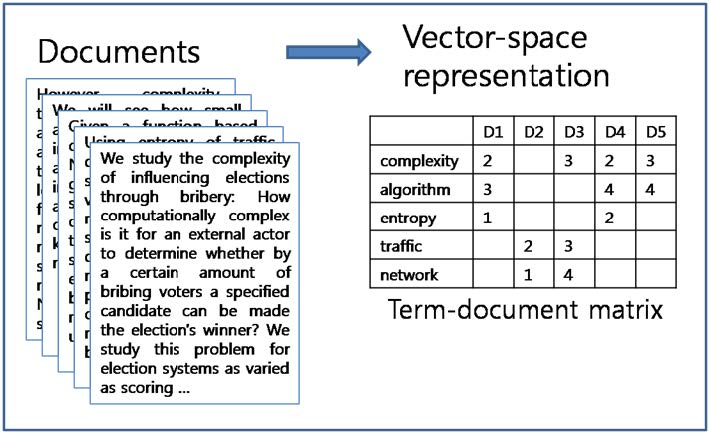
\includegraphics[width=8cm]{fig_4_1.jpg} 
	\caption{Bag-of-Word embedding}\label{fig_4_1}
\end{figure}
\section{Probabilistic Latent Semantic Analysis}
pLSA identifies topics with characteristic distributions over words, which are the model parameters, and models each document as a \textbf{mixture of topics}. Note that the mixing weights are not the uncertainties about certain "correct" topic but show that the document belongs to multiple topics with different "importance". For example, a report about soccer world cup 2022 might contains words from soccer vocabulary (e.g. "teams", "play", "match") in a sense of distribution and words from political vocabulary (e.g. "labor", "corruption", "president") in a sense of distribution. The goal is to discover topics in an unsupervised fashion.
\subsection{Basic Model}
As a predictive model, pLSA samples words in a two-stage manner:
\begin{enumerate}
	\item Sample topic from the mixtures for each token/word.
	\item Sample token/word, given sampled topic
\end{enumerate}
\par As illustrated in Figure \ref{fig_4_2}, different colors correspond to different topics. Given a document $d$, we first sample topics $z_i$ for every position $i$ in the document, and then sample a word $w_i$ conditioning on the topic $z_i$ of that position.
\begin{figure}[h] 
	\centering 
	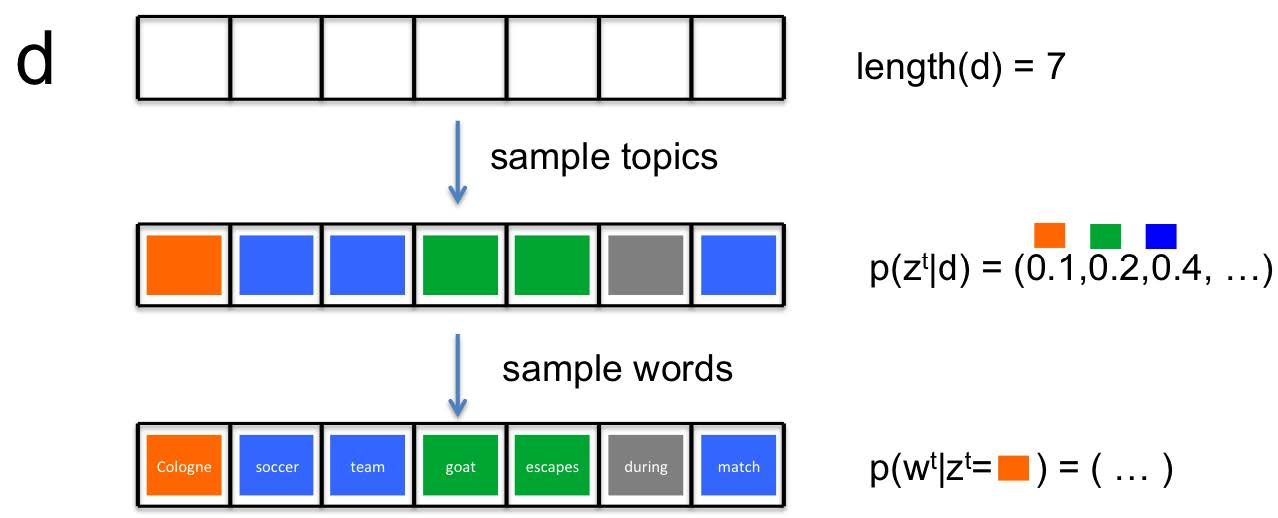
\includegraphics[width=8cm]{fig_4_2.jpg} 
	\caption{Two-stage sampling of pLSA}\label{fig_4_2}
\end{figure}
\par The model parameters are tied up with this two-stage sampling:
\begin{enumerate}
	\item Each document has a specific mix of topics: $p(z|d)$.
	\item Each topic has a specific distribution of words: $p(w|z)$.
\end{enumerate}
\par Given the model parameters, we can compute the log-likelihood of observed data and use some criteria to evaluate how well our model performs. Specifically, we can get the occurrence (probability) of word $w$ in context/document $d$ (also known as context model) by marginalizing out topic $z$ from the conditional joint distribution given $d$:
\begin{equation}\label{eq_4_word_prob}
	p(w|d)=\sum_{z=1}^{K}p(w,z|d)=\sum_{z=1}^{K}p(w|z,d)p(z|d) = \sum_{z=1}^{K}p(w|z)p(z|d)
\end{equation}
where we identify topics with integers $z\in \{1,\dots,K\}$ ($K$: pre-specified), and word $w$ is related to a fixed "slot", i.e. fixed position in the document, and has an identical distribution for every slot. In the last equality above, we made a conditional independence assumption $w\perp d\ |\ z$ for that we assume topics represent regularities common to the entire collection.
\begin{remark}
	As mentioned above, we need to pre-specify the topic number $K$ for pLSA. However, we need to be careful about the interpretability of our model on these "topics". For example, if we apply pLSA with $K=4$ on data collected from 4 topics (say "sports", "politics", "music", and "science"), we may expect our pLSA model to find these topics, but with $K=3$ the "meaning" of topics found by our model may be a lot more unpredictable. 
\end{remark}
\par With (\ref{eq_4_word_prob}) and an additional assumption that every word in a document is independent of each other, the log-likelihood can be computed in 2 possible views:
\begin{itemize}
	\item Summarize data into co-occurrence counts ${\bf X}=x_{ij}$ (number of occurrences of $w_j$ in document $d_i$)
	\item Alternatively: multiset $\mathcal{X}$ over index pair $(i,j)$, e.g. 
	$$\mathcal{X} = \{(1,1), (1,1), (1, 2),\dots\}$$
\end{itemize} 
The log-likelihood, therefore, is
\begin{equation}\label{eq_4_log_l}
	l({\bf U},{\bf V})=\sum_{i,j}x_{ij}\log p(w_j|d_i)=\sum_{(i,j)\in \mathcal{X}}\log \sum_{z=1}^{K} \underbrace{p(w_j|z)}_{=:v_{zj}}\underbrace{p(z|d_i)}_{=:u_{zi}}
\end{equation}
where $u_{zi}\geq 0$ and $v_{zj}\geq 0$ are model parameters. Since they are probability distributions, we further require constraints:
\begin{equation*}
	\sum_z u_{zi}=1\ (\forall i),\ \sum_j v_{zj}=1\ (\forall z)
\end{equation*}
\par A natural attempt is to optimize (\ref{eq_4_log_l}) via gradient descent, but the sum of probabilities inside the log can cause problem. In the following, we will address the problem from another view, namely the Expectation Maximization, which iteratively optimizes a lower bound of the original objective function. Since it's a very useful algorithm and is closely related to another topic we will meet in the sequel, the k-means algorithm, we will introduce more of EM in details in the next section, while it might be out of the scope of this course.
\subsection{Expectation Maximization for pLSA}
EM deals with the hardness of maximization of the original log-likelihood function by assuming latent variables and bring them back to play, which is known as complete data model. Denote all observed variables (i.e. words in topic model) as ${\bf X}$, all latent variables as ${\bf Z}$, and model parameters as $\theta$. Then, $\{{\bf X, Z}\}$ represents the complete data set, while $\{{\bf X}\}$ is called incomplete data set. In this case, we shall suppose that optimization of the $p({\bf X}|\theta)$ is hard but easy for $p({\bf X, Z}|\theta)$. This will be discussed in detail in the next section.
\par In pLSA, we introduce missing data $Q_{zij}\in\{0,1\}$ indicating that $w_j$ in $d_i$ is generated via $z$. Note that by construction: $\sum_{z}Q_{zij}=1$. Then this naturally yields corresponding variational parameters (latent variables), which is a distribution over $z$:
\begin{equation*}
	q_{zij}=\mathbb{P}(Q_{zij}=1),\ \sum_{z} q_{zij}=1
\end{equation*}
With $q_{zij}$, we can lower bound $\log p(w_j|d_i)$ in (\ref{eq_4_log_l}) via Jensen's inequality. First re-write it into a convex combination, using that $q_{zij}\geq 0,\ \sum_{z} q_{zij}=1$:
\begin{equation*}
	\log p(w_j|d_i) = \log \sum_{z=1}^{K} u_{zi}v_{zj} =  \log \sum_{z=1}^{K} q_{zij}\frac{u_{zi}v_{zj}}{q_{zij}}
\end{equation*}
Then since $\log(\cdot)$ is a concave function, Jensen's inequality gives:
\begin{equation}\label{eq_4_lwb}
	\log p(w_j|d_i) =\log \sum_{z=1}^{K} q_{zij}\frac{u_{zi}v_{zj}}{q_{zij}} \geq \sum_{z=1}^{K} q_{zij}[\log u_{zi} + \log v_{zj} - \log q_{zij}]
\end{equation}
Optimizing over $q$ for fixed $u_{zi},v_{zj}$ maximizes the lower bound (\textbf{Expectation Step}). To solve for optimal $q$, we can apply Lagrangian:
\begin{equation*}
	\mathcal{L}(q, \lambda) = \sum_{z=1}^{K} q_{zij}[\log u_{zi} + \log v_{zj} - \log q_{zij}] + \lambda (\sum_{z} q_{zij}-1)
\end{equation*}
Apply the first order optimality condition, we get
\begin{equation*}
	\lambda + (\log u_{zi}v_{zj} - \log q_{zij} -1) \overset{set}{=}0
\end{equation*}
with normalization constraint we get
\begin{equation*}
	q_{zij} = \frac{u_{zi}v_{zj}}{\sum_{z=1}^{K}u_{zi}v_{zj}} = \frac{p(w_j|z)p(z|d_i)}{\sum_{z=1}^{K}p(w_j|z)p(z|d_i)}
\end{equation*}
which turns out to be the posterior of $Q_{zij}$ under current model ($\{u_{zi},v_{zj}\}$). The interpretation of the expectation step is clear: if given $u_{zi},v_{zj}$ we can solve for the optimal $q$. But since we don't know the true model parameters in advance, we need to do it iteratively with the following \textbf{Maximization Step}, which solves for the optimal parameters with fixed $q$. First apply lower bound (\ref{eq_4_lwb}) to the log-likelihood (\ref{eq_4_log_l}):
\begin{equation*}
	l({\bf U},{\bf V}) \geq \sum_{i,j}x_{ij} \sum_{z=1}^{K} q_{zij}[\log u_{zi} + \log v_{zj} - \log q_{zij}]
\end{equation*}
Then again we can apply Lagrangian to solve for optimal $u_{zi}$ and $v_{zj}$. With a similar derivation, we get
\begin{equation*}
	u_{zi}=\frac{\sum_{j}x_{ij}q_{zij}}{\sum_{j}x_{ij}},\quad v_{zj}=\frac{\sum_{i}x_{ij}q_{zij}}{\sum_{i,l}x_{il}q_{zil}}
\end{equation*}
where in the first equality we used $\sum_{z} q_{zij}=1$. Note that the denominators of the two expressions differs simply because $u_{zi}$ is a distribution over $z$ and $v_{zj}$ is a distribution over $j$. Also, we see that the numerators are simple weighted counts, and the denominators ensure proper normalization.
\par EM for MLE in pLSA gives a simple alternating scheme for finding a solution and is guaranteed to converge. However, EM is not guaranteed to find global optimum.
\section{Expectation Maximization in a section}\label{sec_4_EM}
This section is not relevant to this course and is written for my personal interests. So feel free to skip it! The content mainly comes from chapter 9 of one of my favorite books, \emph{Pattern Recognition and Machine Learning} by Christopher M. Bishop. I recommend ones who are interested in more materials to read the corresponding chapters.
\subsection{K-means Clustering}
One of the most popular clustering methods is k-means algorithm. Given $x_1,\dots,x_n\in \mathbb{R}^d$, the k-means algorithm partitions the data points into k disjoint "groups" $S_1,\dots,S_k$ with centers $\mu_1,\dots,\mu_k\in \mathbb{R}$, which can be seen as prototypes of each "group". In another word, k-means defines the following optimization problem:
\begin{equation*}
	\min_{\{S_k\},\{\mu_k\}}\sum_{k=1}^{K}\sum_{n\in S_k}\|x_n-\mu_k\|^2
\end{equation*}
or equivalently
\begin{equation*}
\min_{\{r_{nk}\},\{\mu_k\}}\sum_{k=1}^{K}\sum_{n=1}^{N}r_{nk}\|x_n-\mu_k\|^2
\end{equation*}
where $r_{nk}\in \{0,1\}$ is a binary indicator variable describing which of the $K$ cluster the data $x_n$ is assigned to. Since directly optimizing k-means objective is NP-hard, we usually apply an iterative scheme, which is also known as Lloyd's algorithm:
\begin{itemize}
	\item Given centers $\mu_1,\dots,\mu_K$, assign each point to the closest center:
	\begin{equation*}
		r_{nk}=\begin{cases}
		1& \text{if }k=\arg\min_j\|x_n-\mu_j\|^2\\
		0& \text{otherwise.}
		\end{cases}
	\end{equation*}
	\item Given all the assignments, find the optimal centers:
	\begin{equation*}
		\mu_k = \frac{1}{|S_k|}\sum_{n\in S_k}x_n.
	\end{equation*}
\end{itemize}
We shall see that these two stages of updating $r_{nk}$ and updating $\mu_k$ correspond to the E steps and M steps of the EM algorithm, respectively.
\subsection{Mixtures of Gaussians}
We now turn to a formulation of Gaussian mixtures in terms of discrete latent variables, which will serve to motivate the EM algorithm. A Gaussian mixture distribution can be written in a form of linear superposition of Gaussians:
\begin{equation*}
	p({\bf x})=\sum_{k=1}^{K} \pi_k \mathcal{N}({\bf x}|\bm{\mu}_k, {\bf\Sigma}_k).
\end{equation*}
Let us introduce a K-dimensional binary random variable ${\bf z}$ satisfying that $z_k\in \{0,1\}$ and $\sum_k z_k=1$. Then we can define the joint distribution $p({\bf x,z})$ using a marginal distribution $p({\bf z})$ and a conditional distribution $p({\bf x}|{\bf z})$. $p({\bf z})$ is specified in terms of the mixing coefficients $\pi_k$, such that
\begin{equation*}
	p(z_k=1)=\pi_k \in [0,1],\ \sum_k\pi_k=1
\end{equation*}
which yields
\begin{equation*}
	p({\bf z})=\prod_{k}\pi_k^{z_k}.
\end{equation*}
On the other hand, the conditional distribution of ${\bf x}$ given a specific ${\bf z}$, note that ${\bf z}$ only has K different states, is given by
\begin{equation*}
	p({\bf x}|z_k=1)=\mathcal{N}({\bf x}|\bm{\mu}_k,{\bf \Sigma}_k)
\end{equation*}
which is equivalent to
\begin{equation*}
	p({\bf x}|{\bf z}) = \prod_k \mathcal{N}({\bf x}|\bm{\mu}_k,{\bf \Sigma}_k)^{z_k}.
\end{equation*}
The marginal distribution of ${\bf x}$ is then obtained by summing the joint distribution $p({\bf x,z})=p({\bf z})p({\bf x}|{\bf z})$ over all possible states of ${\bf z}$:
\begin{equation*}
	p({\bf x}) = \sum_z p({\bf z})p({\bf x}|{\bf z}) =  \sum_z \prod_k (\pi_k \mathcal{N}({\bf x}|\bm{\mu}_k,{\bf \Sigma}_k))^{z_k} = \sum_{k} \pi_k \mathcal{N}({\bf x}|\bm{\mu}_k, {\bf\Sigma}_k).
\end{equation*}
We have therefore found an equivalent formulation of the Gaussian mixture involving an explicit latent variable. This allow us to work with the joint distribution $p({\bf x, z})$ instead of $p({\bf x})$, which will lead to significant simplifications. Another quantity that will play an important role is $p({\bf z|x})$. We use $\gamma(z_k)$ to denote $p(z_k=1|{\bf x})$, whose value can be found using Bayes' theorem:
\begin{align*}
	\gamma(z_k) \equiv p(z_k=1|{\bf x})= \frac{p(z_k=1)p({\bf x}|z_k=1)}{\sum_i p(z_i=1)p({\bf x}|z_i=1)}= \frac{\pi_k \mathcal{N}({\bf x}|\bm{\mu}_k, {\bf\Sigma}_k)}{\sum_{i} \pi_i \mathcal{N}({\bf x}|\bm{\mu}_i, {\bf\Sigma}_i)}.
\end{align*}
$\gamma(z_k)$ has an interpretation as the \emph{responsibility} that component $k$ takes for "explaining" the observation ${\bf x}$. 
\par Now we represent the data that we want to model with Gaussian mixtures by ${\bf X}\in \mathbb{R}^{N\times D}$ with the $n^{\text{th}}$ row is given by ${\bf x}_n^T$, and the latent variables by ${\bf Z}\in \mathbb{R}^{N\times K}$ with the $n^{\text{th}}$ row ${\bf z}_n^T$. Assume that the data points are independently drawn from the distribution, the log-likelihood therefore is given by
\begin{equation}\label{eq_4_log_l_gm}
	\ln p({\bf X}|\bm{\pi},\bm{\mu},{\bf \Sigma}) = \sum_{n=1}^{N}\ln \left\{\sum_{k=1}^{K} \pi_k \mathcal{N}({\bf x}|\bm{\mu}_k, {\bf\Sigma}_k)\right\}.
\end{equation}
The difficulty of maximizing (\ref{eq_4_log_l_gm}) arises from the presence of the summation over $k$ that appears inside the logarithm. If we set the derivative to zero, we can no longer get a close form solution.
\subsection{EM for Gaussian mixtures}
\emph{Expectation-maximization} is an elegant and powerful method for finding maximum likelihood solutions for models with latent variables. First we will discuss EM in the context of Gaussian mixtures, and later in a more general view.
\par The conditions that must be satisfied for an optimal solution is the first order optimality condition. Setting the derivatives of (\ref{eq_4_log_l_gm}) with respect to $\bm{\mu}_k$ and ${\bf \Sigma}_k$ to zero, we obtain
\begin{align}
	\label{eq_4_mu}&\frac{\partial (\ref{eq_4_log_l_gm})}{\partial \bm{\mu}_k}=0\Rightarrow \bm{\mu}_k = \frac{1}{N_k}\sum_{n=1}^{N}\gamma(z_{nk}){\bf x}_n\\
	 \label{eq_4_sigma}&\frac{\partial (\ref{eq_4_log_l_gm})}{\partial {\bf \Sigma}_k}=0\Rightarrow {\bf \Sigma}_k=\frac{1}{N_k}\sum_{n=1}^{N}\gamma(z_{nk}) ({\bf x}_n-\bm{\mu}_k)({\bf x}_n-\bm{\mu}_k)^T\\
	 \label{eq_4_gamma}&N_k = \sum_{n=1}^{N}\gamma(z_{nk}), \quad\gamma(z_{nk}) = \frac{\pi_k \mathcal{N}({\bf x}_n|\bm{\mu}_k,{\bf \Sigma}_k)}{\sum_i\pi_i \mathcal{N}({\bf x}_n|\bm{\mu}_i,{\bf \Sigma}_i)} 
\end{align}
where we have assumed that ${\bf \Sigma}_k$ is invertible for all $k$, and $N_k$ has a interpretation as the effective number of point assigned to cluster $k$. From the form of this solution we see that $\bm{\mu}_k$ and ${\bf \Sigma}_k$ are weighted version of mean and variance of the data set, and the weighting factor for ${\bf x}_n$ is given by the posterior probability $\gamma(z_{nk})$ that component $k$ was responsible for generating ${\bf x}_n$.
\par Finally, we maximize (\ref{eq_4_log_l_gm}) w.r.t. the mixing coefficients $\pi_k$. Note that $\pi_k$ needs to be non-negative and normalized. We use a Lagrange multiplier to force the normalization constraint and show that the solution satisfies the non-negative constraint automatically. Define the following Lagrangian
\begin{equation*}
	\mathcal{L}=\ln p({\bf X}|\bm{\pi},\bm{\mu},{\bf \Sigma}) + \lambda\left(\sum_k \pi_k-1\right).
\end{equation*}
Set it's derivative to zero w.r.t. $\pi_k$ and use the normalization constraint we obtain
\begin{equation}\label{eq_4_pi}
	\pi_k = \frac{N_k}{N} 
\end{equation}
which has a clear interpretation as the average responsibility that component $k$ takes for explaining the data points. It is worth emphasizing that the results (\ref{eq_4_mu}), (\ref{eq_4_sigma}), and (\ref{eq_4_pi}) are not closed form solutions for the model parameters because of the dependency of the responsibilities $\gamma(z_{nk})$ on these parameters. However, these results suggest a simple iterative scheme for finding a solution, which we will see turns out to be an instance of the EM algorithm. 
\par We first initialize all the model parameters, and then alternate between the following two updates until some conditions are satisfied:
\begin{itemize}
	\item  \textbf{E (expectation) step}: Use the current model parameters $\{\bm{\pi}, \bm{\mu}, {\bf \Sigma}\}$ to evaluate the posterior probabilities/responsibilities $\gamma(z_{nk})$ via (\ref{eq_4_gamma}).
	\item  \textbf{M (maximization) step}: Use the updated responsibilities $\gamma(z_{nk})$ to re-estimate model parameters $\{\bm{\pi}, \bm{\mu}, {\bf \Sigma}\}$ via (\ref{eq_4_mu}), (\ref{eq_4_sigma}), and (\ref{eq_4_pi}).
\end{itemize}
We shall see that in each update the parameters resulting from an E step followed by an M step is guaranteed to increase the log-likelihood function. Since the log-likelihood function is always upper-bounded by 0, EM is therefore guaranteed to converge in general since EM maximizes a lower bound for the log-likelihood in each step.
\subsection{An Alternative View of EM}\label{sec_4_em_km_compare}
In this section, we will discuss th EM algorithm in a more general setting. The goal of the EM algorithm is to find maximum likelihood solutions for models having latent variables. We denote the set of all observed data by ${\bf X}$ with the $n^{\text{th}}$ row representing ${\bf x}_n^T$, and similarly we denote the set of all latent variables by ${\bf Z}$ with a corresponding row ${\bf z}_n^T$. Given the set of all model parameters denoted by $\bm{\theta}$, the log-likelihood of ${\bf X}$ is
\begin{equation*}
	\ln p({\bf X}|\bm{\theta}) = \ln \left(\sum_{\bf Z} p({\bf X,Z}|\bm{\theta}) \right).
\end{equation*}
The hardness of optimizing this objective arises from summation over the latent variables inside the logarithm. Now suppose that, for each observation ${\bf X}$, we were told the corresponding value of the latent variable {\bf Z}. We shall call $\{{\bf X, Z}\}$ the \emph{complete} data set, and refer to the actual observed data ${\bf X}$ as \emph{incomplete}. We shall suppose that maximization of the complete-data log likelihood function $\ln p({\bf X,Z}|\bm{\theta})$ is straightforward.
\par In practice, we are not given the complete data set $\{{\bf X, Z}\}$, and our knowledge of the values of the latent variables ${\bf Z}$ is given only by the posterior distribution $p({\bf Z}|{\bf X},\bm{\theta})$. Because we cannot use the complete-data log-likelihood, we consider instead its expected value under the posterior distribution of the latent variable, which corresponds to the E step of the EM algorithm. In the subsequent M step, we maximize this expectation. If the current estimate for the parameters is denoted $\bm{\theta}^{\text{old}}$, then a pair of successive E and M steps gives rise to a revised estimate $\bm{\theta}^{\text{new}}$. The parameters are initialized by $\bm{\theta}_0$.
\par In the E step, we use the current model parameters $\bm{\theta}^{\text{old}}$ to find the posterior distribution $p({\bf Z}|{\bf X},\bm{\theta}^{\text{old}})$, and use this distribution to find the expectation of the complete-data log-likelihood for some general parameter value $\bm{\theta}$:
\begin{equation*}
	\mathcal{Q}(\bm{\theta}, \bm{\theta}^{\text{old}}) = \sum_{\bf Z} p({\bf Z}|{\bf X},\bm{\theta}^{\text{old}}) \ln p({\bf X, Z}|\bm{\theta}).
\end{equation*}
\par In the M step, we determine the revised parameter estimate $\bm{\theta}^{\text{new}}$ by maximizing this function
\begin{equation*}
	 \bm{\theta}^{\text{new}} = \mathop{\arg\max}_{\bm{\theta}} 	\mathcal{Q}(\bm{\theta}, \bm{\theta}^{\text{old}}).
\end{equation*}
Note that in the definition of $\mathcal{Q}(\bm{\theta}, \bm{\theta}^{\text{old}})$, the summation is outside of the logarithm, so, by assumption, the M step will be tractable.
\subsubsection{Gaussian Mixtures Revisited}
We now consider the application of this latent variable view of EM to the Gaussian mixture model. With the same notation as before, the likelihood for the complete data set takes the form
\begin{equation}\label{eq_4_g_rev_joint}
	p({\bf X,Z}|\bm{\pi},\bm{\mu},{\bf \Sigma}) = \prod_{n=1}^{N}\prod_{k=1}^{K} \left(\pi_k \mathcal{N}({\bf x}_n|\bm{\mu}_k,{\bf \Sigma}_k)\right)^{z_{nk}}
\end{equation}
which yields the corresponding log-likelihood
\begin{equation*}
	\ln p({\bf X,Z}|\bm{\pi},\bm{\mu},{\bf \Sigma}) = \sum_{n=1}^{N}\sum_{k=1}^{K} z_{nk}\left(\ln \pi_k +\ln \mathcal{N}({\bf x}_n|\bm{\mu}_k,{\bf \Sigma}_k)\right)
\end{equation*}
Using (\ref{eq_4_g_rev_joint}) together with the Bayes rule, we have
\begin{equation*}
	p({\bf Z}|{\bf X}, \bm{\pi},\bm{\mu},{\bf \Sigma}) \propto  \prod_{n=1}^{N}\prod_{k=1}^{K} \left(\pi_k \mathcal{N}({\bf x}_n|\bm{\mu}_k,{\bf \Sigma}_k)\right)^{z_{nk}}
\end{equation*}
and it's not difficult to see that under the posterior distribution the $\{{\bf z}_n\}$ are independent. Using that $z_{nk}=\{0,1\}$ and $\sum_k z_{nk}=1$, the expectation of $z_{nk}$ under the posterior distribution is given by
\begin{align*}
	\mathbb{E}[z_{nk}] &= \sum_{z_{nk}}z_{nk}p(z_{nk}|{\bf x}_n, \bm{\mu}_k, {\bf \Sigma}_k)\\
	&= \sum_{z_{nk}}z_{nk} \frac{p(z_{nk},{\bf x}_n|\bm{\mu}_k, {\bf \Sigma}_k)}{\sum_{z_{nj}}p(z_{nj},{\bf x}_n|\bm{\mu}_j, {\bf \Sigma}_j)}\\
	&= \frac{\sum_{z_{nk}}z_{nk}(\pi_k \mathcal{N}({\bf x}_n|\bm{\mu}_k,{\bf \Sigma}_k))^{z_{nk}}}{\sum_{z_{nj}}(\pi_j \mathcal{N}({\bf x}_n|\bm{\mu}_j,{\bf \Sigma}_j))^{z_{nj}}}\\
	&= \frac{\pi_k \mathcal{N}({\bf x}_n|\bm{\mu}_k,{\bf \Sigma}_k)}{\sum_{j=1}^{K}\pi_j \mathcal{N}({\bf x}_n|\bm{\mu}_j,{\bf \Sigma}_j)} = \gamma(z_{nk}).
\end{align*}
Note that the sum over $z_{nk}$ only has 2 terms where $z_{nk}=1$ or $z_{nk}=0$. The sum over $z_{nj}$ means given $n$ summing over all possible latent variable ${\bf z}_n$ which takes $K$ different values ($z_{nj}=1$ for one $j \in [K] $). Then the expectation of the complete-data log-likelihood under the posterior distribution w.r.t. the latent variables ${\bf Z}$ is
\begin{equation}\label{eq_4_g_rev_ex}
	\mathbb{E}_{\bf Z}[\ln p({\bf X,Z}|\bm{\pi},\bm{\mu},{\bf \Sigma})] =  \sum_{n=1}^{N}\sum_{k=1}^{K} \gamma(z_{nk})\left(\ln \pi_k +\ln \mathcal{N}({\bf x}_n|\bm{\mu}_k,{\bf \Sigma}_k)\right).
\end{equation}
Now if we apply the EM algorithm we will get exactly the same results as (\ref{eq_4_mu}), (\ref{eq_4_sigma}), and (\ref{eq_4_pi}). Specifically, we first initialize the model parameters $\bm{\mu}^{\text{old}}$, ${\bf \Sigma}^{\text{old}}$, and $\bm{\pi}^{\text{old}}$ for some values, and use these to evaluate the responsibilities (E step). We then maximize (\ref{eq_4_g_rev_ex}) with fixed responsibilities over model parameters.
\subsubsection{Relation to K-means}
Comparison of the K-means algorithm with the EM algorithm for Gaussian mixtures shows a close similarity. The K-means algorithm performs a \emph{hard} assignment of data points to clusters, in which each data point is assigned uniquely to one cluster, while the EM for Gaussian mixtures makes a \emph{soft} assignment based on the posterior probabilities. In fact, we can derive the K-means algorithm as a particular limit of EM for Gaussian mixtures as follows.
\par Consider a Gaussian mixture model with covariance matrix $\epsilon {\bf I},\ \epsilon\rightarrow 0$ for all components. Then we can compute the responsibility for $z_{nk}$ as
\begin{equation}\label{eq_4_k_means_resp}
	\gamma(z_{nk}) = \frac{\pi_k \exp\{-\|{\bf x}_n - \bm{\mu}_k\|^2/2\epsilon\}}
	{\sum_j \pi_j \exp\{-\|{\bf x}_n - \bm{\mu}_j\|^2/2\epsilon\}}.
\end{equation}
If $\epsilon\rightarrow 0$, we see that $\gamma(z_{nk})$ will go to zero except for j which indicates the closest $\bm{\mu}_j$ for ${\bf x}_n$, and $\gamma(z_{nj})$ will go to unity. In this limit, we obtain a hard assignment of points $\gamma(z_{nk})=r_{nk}$, just as in K-means algorithm. Each data point is thereby assigned to the cluster having the closest mean. Applying (\ref{eq_4_k_means_resp}) to (\ref{eq_4_g_rev_ex}), one can show that the EM updates are exactly the same as the k-means updates.
\subsection{The EM Algorithm in General}\label{sec_4_EM_in_gen}
Finally, we briefly discuss the EM algorithm in general. As mentioned, EM is a general technique for finding maximum likelihood solutions for probabilistic models having latent variables. Consider a probabilistic model with observed variables ${\bf X}$, latent variables ${\bf Z}$, and parameters $\bm{\theta}$. Our goal is to maximize the likelihood function given by
\begin{equation*}
	p({\bf X}|\bm{\theta}) = \sum_{{\bf Z}} p({\bf X,Z}|\bm{\theta}).
\end{equation*} 
\par We shall suppose that direct optimization of $p({\bf X}|\bm{\theta})$ is hard but significantly easier for $p({\bf X,Z}|\bm{\theta})$. Next we introduce a distribution $q({\bf Z})$ defined over the latent variables, and then for any choice of $q({\bf Z})$ we have the following decomposition
\begin{equation*}
	\ln p({\bf X}|\bm{\theta}) = \mathcal{L}(q,\bm{\theta})+\text{KL}(q||p).
\end{equation*}
where we have defined
\begin{align}
	\label{eq_4_em_in_g_lb} \mathcal{L}(q,\bm{\theta}) &= \sum_{\bf Z}q({\bf Z})\ln \left\{\frac{p({\bf X, Z}|\bm{\theta})}{q({\bf Z})} \right\}\\
	\text{KL}(q||p)&= -\sum_{\bf Z}q({\bf Z})\ln \left\{\frac{p({\bf  Z}|{\bf X}, \bm{\theta})}{q({\bf Z})} \right\}.
\end{align}
To verify the decomposition we substitute $p({\bf X,Z}|\bm{\theta})=p({\bf X}|\bm{\theta})p({\bf Z}|{\bf X},\bm{\theta})$ into (\ref{eq_4_em_in_g_lb}) to give
\begin{align}
	\mathcal{L}(q,\bm{\theta}) &= \sum_{\bf Z}q({\bf Z})\ln \left\{\frac{p({\bf X}|\bm{\theta})p({\bf Z}|{\bf X},\bm{\theta})}{q({\bf Z})} \right\} \notag\\
	&= \sum_{\bf Z}q({\bf Z})\ln p({\bf X}|\bm{\theta}) + \sum_{\bf Z}q({\bf Z})\ln \left\{\frac{p({\bf  Z}|{\bf X}, \bm{\theta})}{q({\bf Z})} \right\}\notag\\
	\label{eq_4_em_in_g_lbdcp} &= \ln p({\bf X}|\bm{\theta}) - \text{KL}(q||p).
\end{align}
Since we always have $\text{KL}(q||p)\geq 0$, with equality holds if, and only if, $q({\bf Z})=p({\bf Z}|{\bf X},\bm{\theta})$, $\mathcal{L}(q,\bm{\theta})$ is therefore a lower bound of the log-likelihood $ \ln p({\bf X}|\bm{\theta})$ as illustrated in Figure \ref{fig_4_3}.
\begin{figure}[h]
	\centering
	\begin{minipage}[t]{0.42\linewidth}
		\centering
		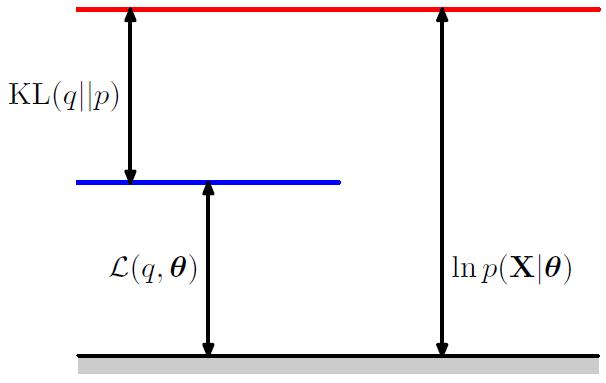
\includegraphics[width=4.5cm]{fig_4_3.jpg}
		\caption{Log-likelihood decomposition.}\label{fig_4_3}
	\end{minipage}
	\begin{minipage}[t]{0.48\linewidth}       
		\centering
		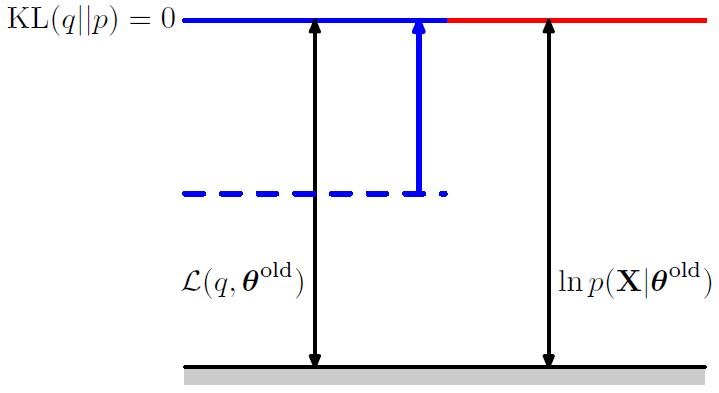
\includegraphics[width=5.4cm]{fig_4_4.jpg}
		\caption{The E step of the EM algorithm.}\label{fig_4_4}
	\end{minipage}
\end{figure}
\par In the E step of the EM algorithm, the lower bound is maximized with respect to $q({\bf Z})$ with $\bm{\theta}=\bm{\theta}^{\text{old}}$ fixed. From (\ref{eq_4_em_in_g_lbdcp}), we can easily see that the maximum is obtained when the KL divergence vanishes since $\ln p({\bf X}|\bm{\theta}^{\text{old}})$ does not depend on $q({\bf Z})$. The E step is illustrated in Figure \ref{fig_4_4}. This means that in the E step, we find the posterior probability $p({\bf Z}|{\bf X},\bm{\theta})$ by maximizing the lower bound $\mathcal{L}(q,\bm{\theta})$ w.r.t. $q({\bf Z})$.
\begin{figure}[h]
	\centering
	\begin{minipage}[t]{0.42\linewidth}
		\centering
		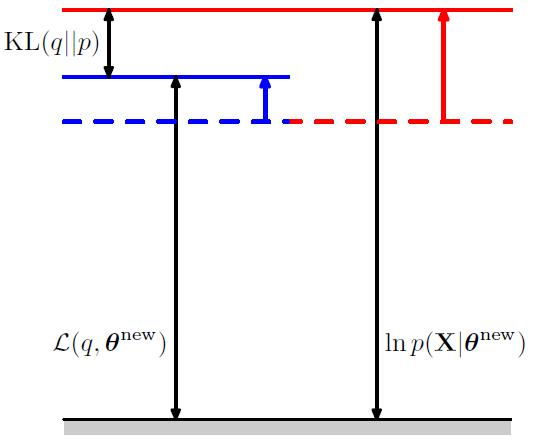
\includegraphics[width=4.5cm]{fig_4_5.jpg}
		\caption{The M step of the EM algorithm.}\label{fig_4_5}
	\end{minipage}
	\begin{minipage}[t]{0.48\linewidth}       
		\centering
		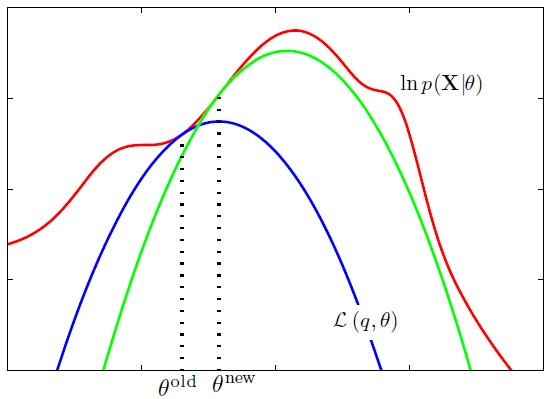
\includegraphics[width=5.4cm]{fig_4_6.jpg}
		\caption{The updates of EM.}\label{fig_4_6}
	\end{minipage}
\end{figure}
\par In the M step, the distribution $q({\bf Z})$ is fixed an the lower bound $\mathcal{L}(q,\bm{\theta})$ is maximized with respect to $\bm{\theta}$ to give some new value $\bm{\theta}^{\text{new}}$. This will cause the lower bound $\mathcal{L}(q,\bm{\theta})$ to increase, and the log-likelihood $\ln p({\bf X}|\bm{\theta}^{\text{new}})$ is therefore increased. However, these two are no longer equal because in general the KL divergence will not be zero after the update. The increase in the log-likelihood is greater than the increase of the lower bound, as shown in Figure \ref{fig_4_5}. If we substitute $q({\bf Z})=p({\bf Z}|{\bf X}, \bm{\theta}^{\text{old}})$ into (\ref{eq_4_em_in_g_lb}), we see that, after the E step, the lower bound takes the form
\begin{align*}
	 \mathcal{L}(q,\bm{\theta}) &= \sum_{\bf Z}p({\bf Z}|{\bf X}, \bm{\theta}^{\text{old}})\ln p({\bf X, Z}|\bm{\theta}) - \sum_{\bf Z}p({\bf Z}|{\bf X}, \bm{\theta}^{\text{old}})\ln p({\bf Z}|{\bf X}, \bm{\theta}^{\text{old}})\\
	 &=\mathcal{Q}(\bm{\theta},\bm{\theta}^{\text{old}})+\text{const}
\end{align*}
where the constant is simply the negative entropy of the $q$ distribution and is therefore independent of $\bm{\theta}$. Thus in the M step, we are maximizing the log-likelihood of the complete-data log-likelihood, just as in the case of the Gaussian mixtures.
\par The operation of the EM algorithm can also be viewed in the space of parameters, as illustrated in Figure \ref{fig_4_6}. The red curve represents the (incomplete-data) log-likelihood, which we want to maximize. We begin at some parameter values $\bm{\theta}^{\text{old}}$, and in the E step we evaluate the posterior distribution of the latent variables, which yields $\mathcal{L}(\bm{\theta},\bm{\theta}^{\text{old}})$, whose value equals to the log-likelihood at $\bm{\theta}^{\text{old}}$ (the blue curve). In the M step, we updates $\bm{\theta}$ by maximizing $\mathcal{L}(\bm{\theta},\bm{\theta}^{\text{old}})$, which gives $\bm{\theta}^{\text{new}}$. The subsequent E step then constructs a bound that is tangential at $\bm{\theta}^{\text{new}}$ as shown by the green curve.
\section{Latent Dirichlet Allocation}
\subsection{Motivation}
In the pLSA model, both dimensions of the data matrix are fixed, which means that with pLSA we can only sample words in the vocabulary for existing documents. To sample new documents, one reasonable extension of pLSA is to allow sampling additional rows of the co-occurrence matrix ${\bf X}$, as illustrated in Figure \ref{fig_4_7}. To do this, we need to be able to sample new topic weights ${\bf u}_i=\{u_{1i},\dots,u_{Ki}\}$ for new documents. Combined with a fixed existing topic-to-word matrix ${\bf V}$, we can predict new data rows. This idea motivates the Latent Dirichlet Allocation (LDA), which acts as a Bayesian improvement of pLSA. 
\begin{figure}[h] 
	\centering 
	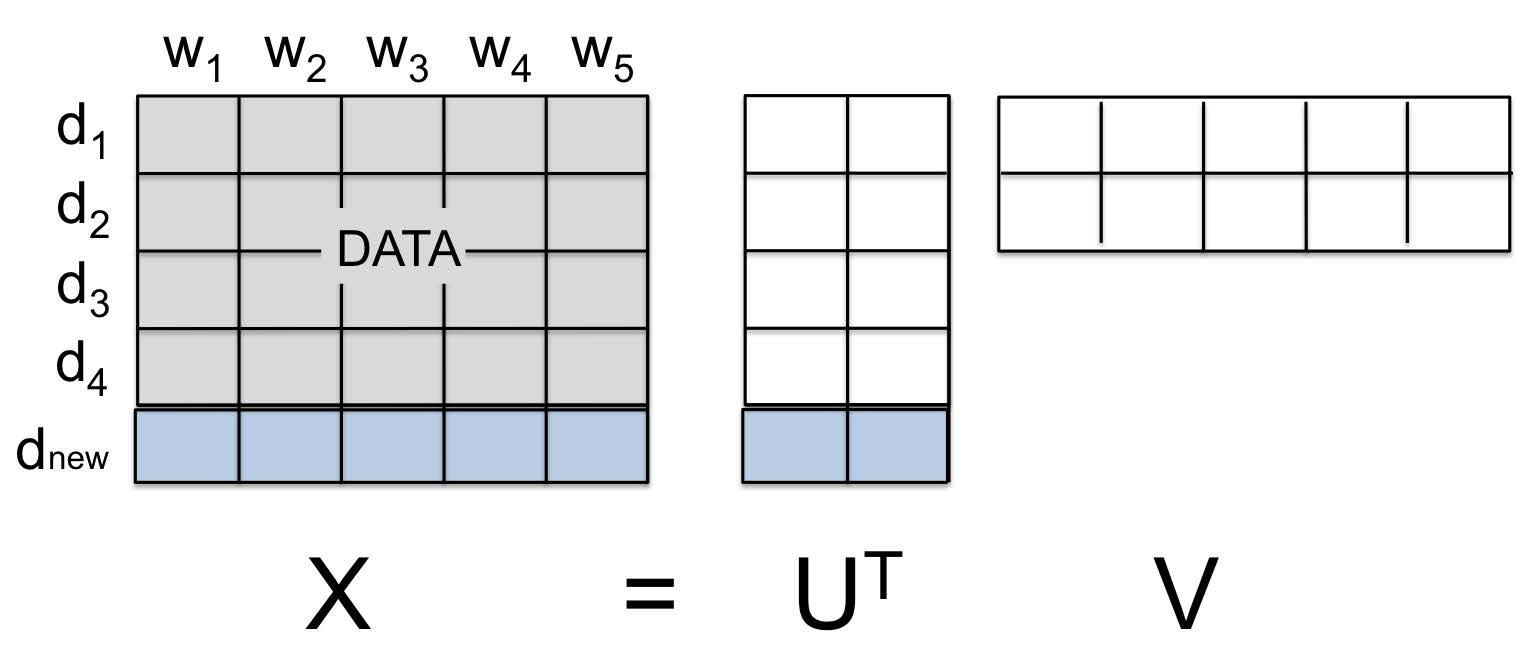
\includegraphics[width=8cm]{fig_4_7.jpg} 
	\caption{We can sample new "documents" by sampling new rows of co-occurrence matrix ${\bf X}$.}\label{fig_4_7}
\end{figure}
\begin{remark}
	If ${\bf X}$ is a count matrix, ${\bf V}$ has to take into account the number of words and can not be a row-normalized probability matrix since we assume $\{{\bf u}_i\}$ are normalized, but if $X_{ij}$ represents $p(w_j|d_i)$, ${\bf V}$ can be a topic-to-word probability matrix. Or, alternatively, we can view the equality in Figure \ref{fig_4_7} as "sampled from".
\end{remark}
\par To sample a new topic weights ${\bf u}_i$, we need to make it a probability vector. The constraints, $u_{ij}\geq 0$ and $\sum_j u_{ij}=1$, indicate that the topics of words that are sampled from ${\bf u}_i$ are subject to a multinomial distribution given a particular document $d_i$. This suggests the choice of Dirichlet distribution as the prior of ${\bf u}_i$ since it's the simplest (conjugate) distribution of a multinomial distribution. The word \emph{conjugate} means a reproducing property: if the prior of parameters is from a Dirichlet distribution with the observations from a multinomial distribution, the posterior distribution of the model parameters will remain a Dirichlet distribution after applying the Bayes rule. Concretely, we have
\begin{equation*}
	p({\bf u}_i|\alpha)\propto\prod_{z=1}^{K}u_{zi}^{\alpha_z-1}
\end{equation*}
where $\alpha\in \mathbb{R}^K$ are hyper-parameters that can be used to generate topic weights. Note that traditionally, $\alpha_z$ has a interpretation as a pseudo count of the number of times that topic $z$ is chosen which in the posterior distribution will be added with the actual count. Given $\alpha$ and the Dirichlet assumption, we can already sample new topic weights, but with this Bayesian setting we can benefit from doing model averaging. Specifically, we can treat ${\bf U}$ as nuisance parameters that need to be averaged out, and ${\bf V}$ are real parameters. Note that ${\bf U}$ can be re-constructed, if needed.
\subsection{Model and Algorithm}
The LDA defines a vector of word counts that can be regarded as a new document. Specifically, the LDA model with fixed document length $l=\sum_j x_j$ defines a multinomial observation model that is given by
\begin{equation*}
p({\bf x}|{\bf V, u})=\frac{l!}{\prod_j x_j!}\prod_j \pi_j^{x_j},\ \pi_j := \sum_z v_{zj}u_z
\end{equation*}
where ${\bf x}$ is the word count vector, and $l!/\prod_j x_j!$ is the corresponding normalization factor of a multinomial distribution. Then performing Bayesian averaging over the topic weights ${\bf u}$ yields
\begin{equation*}
	p({\bf x}|{\bf V}, \alpha) = \int p({\bf x}|{\bf V, u}) p({\bf u}|\alpha)d{\bf u}.
\end{equation*}
It corresponds to the following generative model:
\begin{itemize}
	\item For each document $d_i$: sample ${\bf u}_i\sim \text{Dirichlet}(\alpha)$, where the $\alpha$ are often chosen trivially. Note that the ${\bf u}_i$ will be integrated out in Bayesian averaging when we compute the marginal distribution of word count vectors generated from a LDA model.
	\item For each word slot $w^t,\ 1\leq t\leq l_i$, we do the followings in a i.i.d. manner (therefore we can simply treat all word slots by producting them together):
	\begin{itemize}
		\item Sample topic $z^t \sim \text{Multi}({\bf u}_i)$, which is latent and will be summed out in the marginal distribution of word count vectors generated from this LDA model.
		\item Sample the desired observation $w^t\sim \text{Multi}({\bf v}_{z^t})$.
	\end{itemize}
\end{itemize}
\par There are several algorithms that can be used for LDA. However, since they are beyond the scope of this course, we just list some of them here:
\begin{itemize}
	\item variational expectation maximization
	\item Markov Chain Monte Carlo (MCMC): collapsed Gibbs sampling
	\item distributed, large-scale implementations (100Ms of documents)
\end{itemize}
\section{Non-Negative Matrix Factorization}
As illustrated in Figure \ref{fig_4_7}, pLSA can be regarded as an instance of Non-Negative Matrix Factorization (NMF). Although it seems that we are just add some additional constraints like non-negativity to a standard matrix factorization problem, as we will see in the sequel, NMF has a quite different nature compared with standard MF.
\par In many cases, such as pLSA, we are dealing with a count matrix (take image reconstruction as an example where we do not deal with a count matrix), and we want to model it in a two-set setting (like topic-word and user-item) with some product of probabilities. We first normalize the rows of the count matrix as ${\bf X}\in \mathbb{R}^{N\times M}_{\geq 0}$, and we try to find the NMF of ${\bf X}$:
\begin{equation*}
	{\bf X}\approx {\bf U}^T{\bf V},\ x_{ij}=\sum_{z}u_{zi}v_{zj}=\langle{\bf u}_i,{\bf v}_j\rangle\in [0,1]
\end{equation*}
where we have the follow constraints on matrix factors ${\bf U}$ and ${\bf V}$:
\begin{itemize}
	\item Non-negativity: all parameters are probabilities.
	\item Normalization: ${\bf U}$ is $L_1$ column-normalized, and ${\bf V}$ is row-normalized.
\end{itemize}
The approximation quality is measured via log-likelihood of the original count matrix ${\bf X}_{count}\in \mathbb{Z}^{N\times M}_{\geq 0}$. NMF, just as standard MF, acts also as a dimension reduction method since $N\cdot M\gg (N+M)K-N-M$, where the minus terms come from the normalization constraints.
\par There are also variations of NMF, one of which is to do a non-negative matrix approximation, i.e. qualifying the approximation to ${\bf X}$ via quadratic cost function without normalization constraints on ${\bf U,V}$. Specifically, we want to solve the following optimization problem:
\begin{equation}\label{eq_4_NMF_q_obj}
	\min_{{\bf U,V}}J({\bf U,V})=\frac{1}{2}\|{\bf X}-{\bf U}^T{\bf V}\|_F^2,\ \text{s.t. } u_{zi},v_{zj}\geq 0\ (\forall i,j,z).
\end{equation}
This is a similar problem as pLSA, but they are different in the sense of
\begin{itemize}
	\item different sampling models: quadratic cost function arises naturally from maximum (log) likelihood estimation with Gaussian random variables, while in pLSA we assume a multinomial distribution on observations;
	\item different objectives: we use quadratic loss instead of KL divergence (for details see the remark below);
	\item different constraints: we do not assume normalized parameters.
\end{itemize}
\begin{remark}
	Maximizing the log-likelihood of pLSA model has another interpretation as minimizing a weighted sum of KL divergence between our model predictions and the empirical data distributions. Recall that the log-likelihood of pLSA takes the form of
	\begin{equation*}
		l({\bf U,v})=\sum_{i}\sum_{j}x_{ij} \ln p(w_j|d_i).
	\end{equation*}
	Define $l_i=\sum_j x_{ij}$ as the number of words in $d_i$, and we can re-write the log-likelihood as
	\begin{align*}
		l({\bf U,v})&=\sum_{i}l_i\sum_{j}\frac{x_{ij}}{l_i}\ln p(w_j|d_i)\\
		&= \sum_{i}l_i\sum_{j} p'(w_j|d_i)\left\{\ln \frac{p(w_j|d_i)}{p'(w_j|d_i)} +\ln p'(w_j|d_i)\right\}\\
		&= -\sum_{i}l_i {\rm KL}(p'_{i}||p_i) + {\rm const}
	\end{align*}
	where $p'(w_j|d_i) = x_{ij}/l_i$ is the empirical probability of $w_j$ in $d_i$, and $p'_i$ and $p_i$ are empirical and predictive distribution of words in $d_i$ respectively. We see that maximizing of the log-likelihood is equivalent to minimize a weighted sum of KL divergences between $p'_i$ and $p_i$, and the weight factors are numbers of words in documents. Note that the constant term is independent of the model parameters.
\end{remark}
\begin{figure}[h] 
	\centering 
	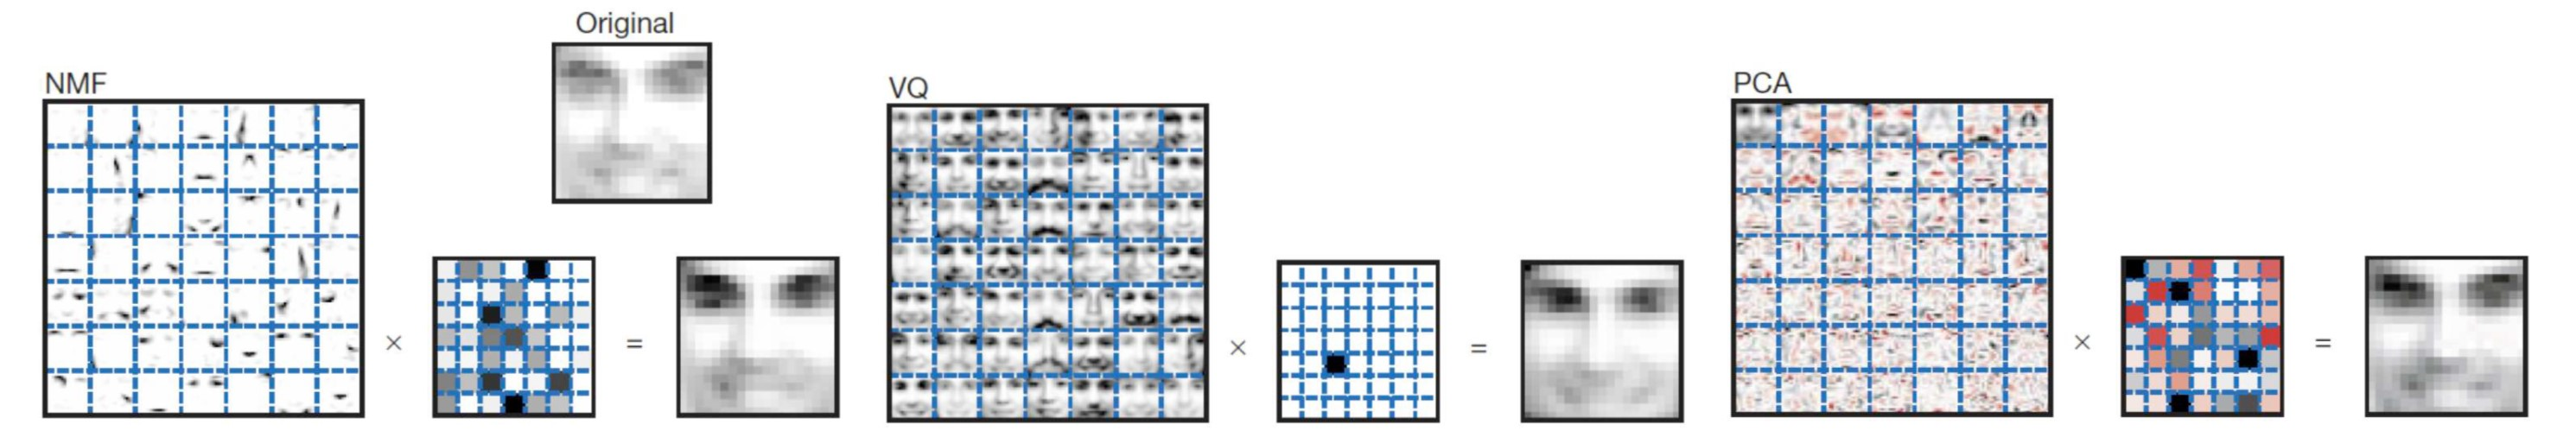
\includegraphics[width=12.5cm]{fig_4_8.jpg} 
	\caption{Different factorization methods for face reconstruction: NMF (left), Vector Quantization (middle), PCA (right).}\label{fig_4_8}
\end{figure}
\par We can see the different nature of factorization methods from the part-based face representation example, as illustrated in Figure \ref{fig_4_8}. NMF is useful when modelling non-negative data (e.g. images, which are non-negative intensities), and since the non-negative constraint requires the model to do additive superpositions without cancellations, NMF learns to represent faces with a set of basis images resembling parts of face, unlike VQ and PCA (see the left picture of Figure \ref{fig_4_8}). However, it is purely a design choice whether to introduce the non-negative constraint.

\par Let us go back to the NMF with quadratic costs and combine things we have covered to see how we can optimize this objective. Since the objective (\ref{eq_4_NMF_q_obj}) is convex in ${\bf U}$ given ${\bf V}$ and vice versa, but not jointly in $({\bf U,V})$, we can choose alternating least squares for optimization. Specifically, we do a alternate optimization of ${\bf U}$ and ${\bf V}$, keeping the other fixed. Given a fixed ${\bf U}$, we can solve for the optimal ${\bf V}$ by re-writing (\ref{eq_4_NMF_q_obj}) as
\begin{align*}
	\min_{\bf V}\frac{1}{2}\|{\bf X}-{\bf U}^T{\bf V}\|_F^2 &=\min_{\bf V} \frac{1}{2}\sum_{i,j}(x_{ij}-{\bf u}_i^T{\bf v}_j)^2\\
	&=\min_{\bf V}\frac{1}{2}\sum_j ({\bf X}_j - {\bf U}^T{\bf v}_j)^2\\
	&=\frac{1}{2}\sum_j \min_{{\bf v}_j}({\bf X}_j - {\bf U}^T{\bf v}_j)^2
\end{align*}
where $\{{\bf X}_j\}$ are columns of ${\bf X}$. Therefore, we can solve for $\{{\bf v}_j\}$ separately, and each of them can be obtained by solving a standard least-square regression type problem. By expanding the square term and setting the derivative w.r.t. ${\bf v}_j$ to zero we get
\begin{equation*}
	({\bf UU}^T){\bf v}_j = {\bf UX}_j.
\end{equation*}
Applying the same analysis to ${\bf U}$ and writing the outputs in matrix notations yield the \emph{normal equations} given by
\begin{equation*}
	({\bf UU}^T){\bf V} = {\bf UX},\quad \text{and}\quad ({\bf VV}^T){\bf U} = {\bf VX}^T
\end{equation*}
which can be solved via QR-decomposition or gradient descent method. Note that we need to project in between alternations to ensure the non-negativity constraint:
\begin{equation*}
	u_{zi} = \max\{0,u_{zi}\},\quad v_{zj} = \max\{0, v_{zj}\}
\end{equation*}
More detailed discussion of algorithms for NMF can be found in Berry, M.W. et al.: Algorithms and applications for approximate non-negative matrix factorization. Computational Statistics \& Data Analysis, 52(1), 2007, pp.155-173.
\par We conclude this chapter with a brief discussion of pLSA and NMF with quadratic loss: \begin{itemize}
	\item They are matrix factorization obeying non-negativity and (optionally, pLSA) normalization constraints.
	\item They have different different cost functions: multinomial likelihood for pLSA, and quadratic loss for NMF (with quadratic loss).
	\item Both of them use a iterative optimization: EM for pLSA, projected ALS for NMF with quadratic loss.
	\item As matrix factorization, they benefit from the interpretability of factors: topics, parts, etc.
	\item They have a wide range of applications.
\end{itemize}
%%%%%%%%%%%%%%%%%%%%%%%%%%%%%%%%%%%%%%%%%%%%%%%%%%%%%%%
%   New Chapter                                       %
%%%%%%%%%%%%%%%%%%%%%%%%%%%%%%%%%%%%%%%%%%%%%%%%%%%%%%%

\chapter{Word Embeddings}
From this chapter on we will slowly move towards deep learning and neural stuff. As a first step, we will focus on the embeddings, specifically the embeddings of words. Our discussion will mainly focus on two popular algorithms, namely the skip-gram model and the GloVe, both of which, to some degree, find a mapping from the original discrete word space (recall the 1-hot representation we have seen) to a continues vector space with much lower dimension which keeps the semantic information. We will see the embeddings found by these methods have some interesting properties, and show surprising applications in fields like machine translation.
\section{Motivation: Word Embeddings}
Word embedding is a conceptually easy way to motivate the idea of embeddings. To understand natural languages, we usually have to deal with their atomic units of meaning, which are usually symbols like words or phrases. It's similar for music analysis, where in early times we regard each song as a black box and use techniques like collaborate filtering to do things. However, these symbols (words, phrase, or name of songs) rarely carry their meanings "on them", and sometimes we want to open the black boxes by finding representations that encodes semantics or meaning (like acoustic models for music). 
\par For words understanding, it is widely accepted that the meaning of a word is in its use in that language (Wittgenstein, 1953). It is not difficult to see this by thinking of a monolingual dictionary, where we use easy words to explain the hard ones by showing their usages. Motivated by this observation, our goal is then to find semantic representations of words, or symbols, that can say something about the relationship between different symbols given examples of word uses in a corpus (word occurrences). The most straightforward way to do this is to embed the symbols in a vector space, which is the most basic type of representation, and the structure (e.g. angles, distances) of the vector space should relate to word meanings. In another word, the points that are close in that vector space should correspond to words with similar meanings. For example, automobile and car are not similar in terms of lexicology but should be close in a desired embedding vector space. Although we might lose some crispness for the words, we benefit a lot by moving from a discrete space to a continuous space since that it allows us to use all methods for analyzing continuous representations including the Deep Learning, where the first step is always to find a representation for the original data. 
\par Now the problem is left with how can we create such vectors. It might be tempting to do it in a supervised manner, but in general cases we have no access to the "correct" embeddings and have even no ideas how should they look like. This suggest an unsupervised direction, and we need a way to qualify our models. Recall the linear autoencoder in Chapter 1, where we used a reconstructive objective, for word embeddings we can instead make a prediction game, as suggested by the observation that word meanings are in their usages. 
\begin{figure}[h] 
	\centering 
	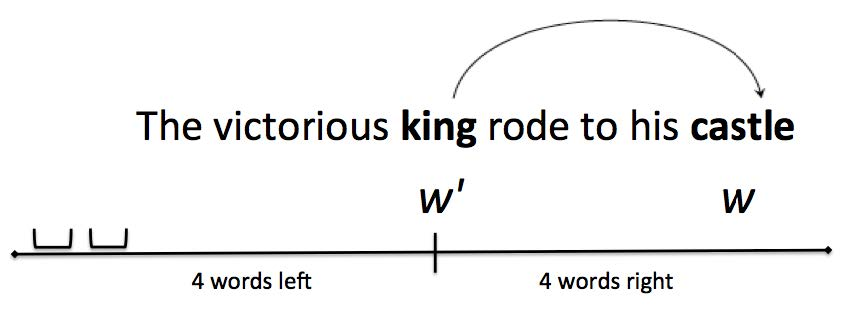
\includegraphics[width=8cm]{fig_5_1.jpg} 
	\caption{An example of the skip-gram model: we choose "king" as the active word and want to predict probabilities of words (say "castle") within a window of size 4.}\label{fig_5_1}
\end{figure}
\begin{figure}[h] 
	\centering 
	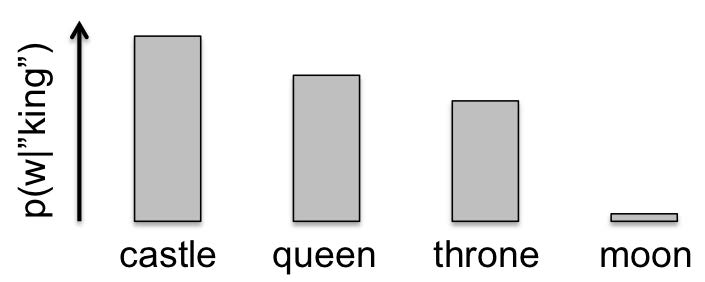
\includegraphics[width=5cm]{fig_5_2.jpg} 
	\caption{The probabilities of some words given word "king". It shows that "castle", "queen", and "throne" appear frequently near "king", and these words are therefore believed to be closely related to "king". We believe that the distribution of co-occurring words itself to some degree determines the lexical semantics}\label{fig_5_2}
\end{figure}
\par Specifically, we want to predict context words given an "active" word, which is known as the Skip-gram Model. The skip-gram model predicts the probability that $w$ occurs in context window of $w'$: $p_{\theta}(w|w')$, which captures statistic dependencies between words, as illustrated in Figure \ref{fig_5_1}. The skip-gram model, as an instance of Distributional Context Models, or Distributional Semantics Models, assumes that the distribution of co-occurring words determines lexical semantics (Figure \ref{fig_5_2}).
\section{Basic Model}
The objective function, or the predictive score, of our model is naturally chosen to be the log-likelihood. Assuming that given $w$, all words within a window are independent of each other, we obtain
\begin{equation}\label{eq_5_log_l}
	\mathcal{L}(\theta;{\bf w})=\sum_{t=1}^{T}\sum_{\Delta \in \mathcal{I}}\log p_{\theta}(w^{(t+\Delta)}|w^{(t)})
\end{equation} 
where $\theta$ represents model parameters and defines the conditional probability distribution over the vocabulary given some words from the vocabulary; ${\bf w}=\{w^{(1)},\dots,w^{(T)}\}$ is the sequence of words and is implicitly padded to handle border cases; $\mathcal{I}=\{-R,\dots,-1,1,\dots,R\}$ defines a window of offsets, where we want to make prediction. Note that alternatively, we can also consider word pairs within the same sentence rather than in some windows.
\begin{remark}
	In the setting of windows, we neglect $p_{\theta}(w|w)$ for word $w$, i.e. $0\notin \mathcal{I}$, because it seems more or less meaningless to consider the word given itself. Although, it does happen that a word appears multiple times within a window, the model described above works out well in practice.
\end{remark}
\par Then we can just perform a maximum likelihood estimation to solve or optimal model parameters $\hat{\theta}$:
\begin{equation*}
	\hat{\theta} = \mathop{\arg\max}_{\theta}\mathcal{L}(\theta;{\bf w})
\end{equation*}
which prefers model that assigns high probability to observed context. Now the remaining question is: how should we define an appropriate model $p_{\theta}(w|w')$? 
\par Recall that we want to find a latent vector representation (embedding) of words. Specifically, our goal is to find the following mapping:
\begin{equation*}
	w \mapsto ({\bf x}_w,b_w)\in \mathbb{R}^{d+1},\quad (\text{vector }+\text{ bias})
\end{equation*}
where for natural languages $d$ is usually chosen to be around $500$, and we will see the advantages to separate the bias term shortly. We hope this vector representation captures the semantics of words, as illustrated in Figure \ref{fig_5_3}. Given 2 vectors, the inner product is one of the simplest thing we can apply and has a nice interpretation in the sense of measuring similarities. We can therefore define the a log-bilinear model that is given by
\begin{equation}\label{eq_5_log_bi}
	\log p_{\theta}(w|w')=\langle {\bf x}_w,{\bf x}_{w'}\rangle + b_w + {\rm const}
\end{equation}
where we use a symmetric bilinear form to fit the log-probabilities, but as we will see later, we can break the symmetry by introducing a different embedding $y_{w'}$ for the "active" word and use $\langle x_w,y_{w'}\rangle$ instead. Recall that in matrix factorization, we often fit the data directly with the inner products, here everything is in a log scale. The bias term gives some words more importance regardless of the conditional word and therefore to some degree handles different word frequency. The last term is a normalization constant. Then we see the log-bilinear model has the following effects:
\begin{itemize}
	\item the unspecific effect: $b_w \uparrow\ \Longrightarrow p_{\theta}(w|w')\uparrow \forall w'$,
	\item the specific effect: $\angle({\bf x}_w,{\bf x}_{w'})\downarrow\ \Longrightarrow p_{\theta}(w|w')\uparrow$.
\end{itemize}
Therefore we can say that in some sense the inner products model the interactions between words, and the biases describe the marginals of each word.
\begin{remark}
	One might ask, if we embed each word with only one vector, will this be a reasonable semantic representation for words with multiple (especially very different) meanings? For example, the word "cloud" has one meaning that is closely related to "sky", as in Figure \ref{fig_5_3}, but also has another meaning which should be closer to "computation". It turns out that in the representation learned by the model we described, the words has close meaning to "sky", as well as words has close meaning to "computation", form a small, i.e. low-dimensional, affine subspace, and the embedding for "cloud" has large inner products with both these two affine subspaces but much smaller for others. Still, multiple representation for a single word is a possible direction for word embedding, but we have to keep in mind that we have no idea what is the right thing to do.
\end{remark}
\begin{figure}[t] 
	\centering 
	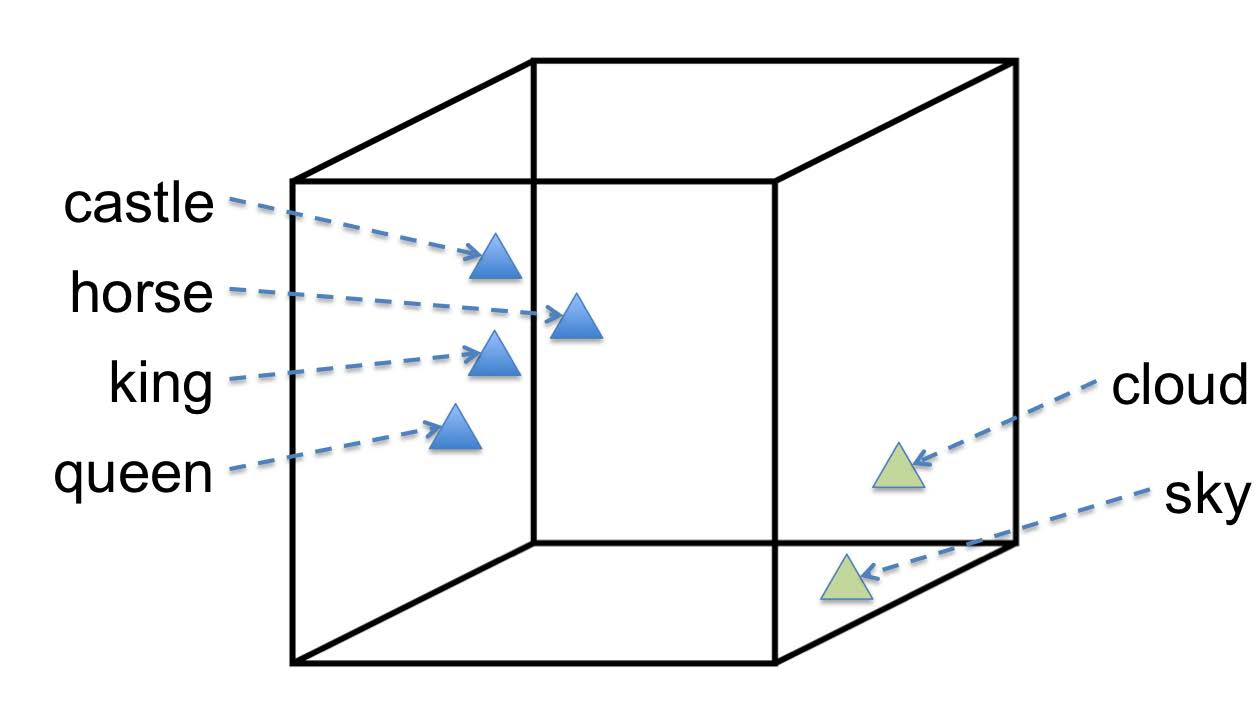
\includegraphics[width=5cm]{fig_5_3.jpg} 
	\caption{An example of words embedded to a vector space that captures semantics.}\label{fig_5_3}
\end{figure}
\par Now we can derive the normalization constant by first neglecting the constant in our log-bilinear model (\ref{eq_5_log_bi}) and exponentiating both side to give
\begin{equation*}
	p_{\theta}(w|w')=\frac{\exp[\langle {\bf x}_w,{\bf x}_{w'}\rangle + b_w]}{Z_{\theta}(w')}
\end{equation*}
where
\begin{equation*}
	Z_{\theta}(w')= \sum_{v\in \mathcal{V}} \exp[\langle {\bf x}_v,{\bf x}_{w'}\rangle + b_v]
\end{equation*}
is a partition function preventing naively making everything large. In the following sections, we will take a closer look into our model and discuss methods to learn the model parameters (word embeddings):
\begin{equation*}
	\theta = (({\bf x}_w,b_w)_{w\in \mathcal{V}})\in \mathbb{R}^{(d+1)\cdot |\mathcal{V}|}.
\end{equation*}
Before we go to the learning algorithms of model parameters, it is worth spending sometime taking another view to understand the role of $b_w$.
\begin{remark}
	The bias term $b_w$ also play a role to avoid ${\bf x}_w$ to be too large, which leads to separate modeling of word interactions and marginals. Since in (\ref{eq_5_log_bi}), there is no explicit regularization on the norm of ${\bf x}_w$, then if we want to evaluate the similarity by computing the inner products of word embeddings we need to be more careful. Consider a toy example in $\mathbb{R}^2$, where we have
	\begin{equation*}
		{\bf x}_1 =(1, 0),\ {\bf x}_2=(1,0.1),\ {\bf x}_2=(1,10)
	\end{equation*}
	and 
	\begin{equation*}
		\langle {\bf x}_1,{\bf x}_2\rangle = \langle {\bf x}_1,{\bf x}_3\rangle.
	\end{equation*}
	Without a bias term, a model may model different importance of words by assigning embeddings with different length. However, an embedding with larger norm will in general lead to larger inner products in magnitude, which will be problematic for the model interpretability. The introduction of $b_w$ helps relieve this problem, and in this case the $\{{\bf x}_w\}$ are usually self-normalized to 1 after training in practice. (This remark is written based on my memory of how Prof Thomas replied to a similar question of mine during the lecture and might not be correct. If you have an idea of how things should be, please send me an e-mail\footnote{yufeiyu@student.ethz.ch} and leave some comments!)
\end{remark}
\section{Skip-Gram Model}
Substituting our log-bilinear model (\ref{eq_5_log_bi}) into the log-likelihood (\ref{eq_5_log_l}) yields
\begin{align*}
	\mathcal{L}(\theta;{\bf w})=\sum_{t=1}^{T}\sum_{\Delta\in \mathcal{I}}[\quad \quad \quad \quad b_{w^{(t+\Delta)}}&\quad {\rm ok} \\
	+ \langle {\bf x}_{w^{(t+\Delta)}},{\bf x}_{w^{(t)}}\rangle&\quad \text{bi-linear}\longleftarrow \#1 \\
	- \log \sum_{v\in \mathcal{V}} \exp[\langle {\bf x}_v,{\bf x}_{w^{(t)}}\rangle + b_v]&\quad \text{large cardinality} \longleftarrow \#2 \\
	&].
\end{align*} 
There are two possible modifications to the basic model: one is on the bi-linear term, where we introduce extra distributions to make our model more flexible; the other one is on the partition function since the current version requires evaluation on a term with very large cardinality in every iteration.
\subsection{Modification \# 1: Context vectors}
As mention before, we can break the symmetry of the bi-linear model by using different embeddings for the conditional word and the words we want to predict. Specifically, we distinguish the output vocabulary $\mathcal{V}$ and the input vocabulary $\mathcal{C}$ and introduce two different embeddings:
\begin{itemize}
	\item ${\bf x}_w$: output embeddings, $w\in \mathcal{V}$
	\item ${\bf y}_w$: input embeddings, $w\in \mathcal{C}$.
\end{itemize}
Thus, we now use a mixed inner product instead:
\begin{equation*}
	\log p_{\theta}(w|w')=\langle {\bf x}_w,{\bf y}_{w'}\rangle + b_w + {\rm const}.
\end{equation*}
By introducing extra parameters we increase the modeling flexibility but also the model dimensionality. We can alternatively apply a simpler model with ${\bf x}_w={\bf y}_w$ for $w\in \mathcal{V}\cap \mathcal{C}$, but it is not very commonly used.
\subsection{Modification \# 2: Objective}
The hardness of optimizing the log-likelihood objective (\ref{eq_5_log_l}) mainly comes from the partition function. A feasible fix for this problem is to alternatively optimizing other objectives whose learned parameters are also optimal for the original problem, such as
\begin{itemize}
	\item contrastive divergence (word2vec, Mikolov et al. 2013)
	\item negative sampling (Mikolov et al. 2013)
	\item pointwise mutual information (Levy \& Goldberg 2014)
	\item weighted squared loss (GloVe, Pennigton et al. 2013)
\end{itemize}
which is still a active area of research. In the following, we will discuss the negative sampling method, and we will see the objective used in GloVe in section \ref{sec_5_glove}.
\subsection{Negative Sampling}
\par The negative sampling, which is a simplified version for a more general method: \emph{noise contrastive estimation} and is used in the original skip-gram paper, reduces the estimation to binary classification tasks. The main idea is to sample positive word pairs from observed data and negative pairs from another distribution, and we train our model to distinguish there pairs. Specifically, we first introduce a contrastive, or negative, distribution $p_n(i,j)$ that is the probability to generate negative examples of word pairs $(w_i,w_j)$ and can be defined quite arbitrarily. Then with the following notations:
\begin{itemize}
	\item observed pairs (taken from some windows)$\Longrightarrow$ positive training examples $\Delta^+$
	\item pairs sampled from $p_n$ $\Longrightarrow$ negative training examples $\Delta^-$
\end{itemize}
we can perform a logistic regression, i.e. maximizing (recall that we have $\sigma(z):=\frac{1}{1+\exp(-z)}$ and $1-\sigma(z)=\sigma(-z)$)
\begin{align}
	\mathcal{L}(\theta) &= \sum_{(i,j)\in \Delta^+} \log p_{\theta} ((i,j)\in\Delta^+) + \sum_{(i,j)\in \Delta^-} \log p_{\theta} ((i,j)\notin\Delta^+) \notag\\
	&=\sum_{(i,j)\in \Delta^+} \log \sigma(\langle {\bf x}_i, {\bf y}_j\rangle) +\sum_{(i,j)\in \Delta^-} \log [1-\sigma(\langle {\bf x}_i, {\bf y}_j\rangle)]\notag\\
	\label{eq_5_ns_lg}&=\sum_{(i,j)\in \Delta^+} \log \sigma(\langle {\bf x}_i, {\bf y}_j\rangle) +\sum_{(i,j)\in \Delta^-} \log \sigma(-\langle {\bf x}_i, {\bf y}_j\rangle)
\end{align}
where we usually still use the bias terms, but for simplicity we have absorbed the bias term into the vectors by
\begin{equation*}
	{\bf x}_i\rightarrow ({\bf x}_i, b_i),\ {\bf y}_j\rightarrow ({\bf y}_j, 1).
\end{equation*}
\par For the choice of negative distribution, it is good to make it reasonably more random, i.e. to have $p_n(i,j)$ with a positive correlation to $P(w_i)P(w_j)$. In the sampling of positive pairs we still first pick an "active" word $w_j$ and sample $w_i$ from a window. It turns out to work well by first re-using the active words $w_j$, and sample "random" context words: $w_i\propto P(w_i)^\alpha$ for some positive $\alpha$, e.g. $\alpha = 3/4$, which magically works well in practice. Although people do not know why this $\alpha = 3/4$ works, it appears to have an effect to exponentially dampen frequent words.
\par Although it might seems to be reasonable to sample as many positive pairs for negative pairs, it turns out an oversampling by a factor $k$ shows better performance in practice, where usually we have $k=2-20$. For larger data sets, people usually use smaller $k$.
\subsubsection{Negative Sampling \& PMI}
Another way to understand what we are doing in negative sampling is by considering what is the best our model can do if it models everything correctly. From the Bayesian view, the best thing we can do for predicting whether a pair is a positive one is to make prediction based on the posterior distribution $p(+|(i,j))$. Applying the Bayes' theorem we obtain
\begin{equation}\label{eq_5_ns_post}
	p(+|(i,j)) = \frac{p(+)p((i,j)|+)}{p(+)p((i,j)|+)+p(-)p((i,j)|-)}
\end{equation}
which yields the Bayesian optimal discriminant for $\mathcal{L}$ define in (\ref{eq_5_ns_lg})
\begin{equation*}
	h^*_{ij}=\sigma^{-1}(p(+|(i,j))) = \log \frac{p(+|(i,j))}{1-p(+|(i,j))}
\end{equation*}
where we have used $\sigma^{-1}(z)=\log \frac{z}{1-z}$. The prior in (\ref{eq_5_ns_post}) is defined by the oversampling rate, i.e. $p(-)/p(+)=k$, and we have
\begin{equation*}
	p((i,j)|+)=p(w_i,w_j),\ p((i,j)|-)=p_n(w_i,w_j).
\end{equation*}
Substituting these into the posterior (\ref{eq_5_ns_post}), we get
\begin{equation*}
	h^*_{ij}=\log\frac{p(w_i,w_j)}{p_n(w_i,w_j)}+\log \frac{1}{k} = \log\frac{p(w_i,w_j)}{p_n(w_i,w_j)}+\log \frac{\kappa}{1-\kappa}
\end{equation*}
where $\kappa=1/(k+1)$. For $k=1$ (no oversampling) and $p_n(w_i,w_j)=p(w_i)p(w_j)$, the optimal embedding therefore satisfies
\begin{equation}\label{eq_5_ns_pmi}
\langle {\bf x}_i,{\bf y}_j \rangle \approx h^*_{ij} = \log\frac{p(w_i,w_j)}{p(w_i)p(w_j)} = {\rm PMI}(w_i,w_j)
\end{equation}
where ${\rm PMI(w_i, w_j)}$ is the \emph{pointwise mutual information} (PMI) between $w_i$ and $w_j$. If we write (\ref{eq_5_ns_pmi}) in a matrix form, we get
\begin{equation*}
	{\bf X}^T{\bf Y}\approx{\rm PMI},\ {\bf X}=({\bf x}_1,\dots,{\bf x}_{|\mathcal{V}|}),\ {\bf Y}=({\bf y}_1,\dots,{\bf y}_{|\mathcal{C}|}).
\end{equation*}
We see that in this case, the negative sampling method actually performs a low-rank approximation to the pointwise mutual information matrix.
\section{GloVe}\label{sec_5_glove}
GloVe uses another strategy to deal with the normalization term. The main idea is to change the problem from maximizing the log-likelihood to a regression problem. Before we discuss the details, let us first introduce some notations. First we summarize the data in a co-occurrence matrix given by
\begin{align*}
	{\bf N}=(n_{ij})&\in \mathbb{N}^{|\mathcal{V}|\cdot |\mathcal{C}|}\\
	n_{ij} = \text{\# occurence of }w_{i}&\in\mathcal{V}\text{ in context of }w_j\in \mathcal{C}.
\end{align*}
Note that ${\bf N}$ is a very sparse matrix with most of its entry $0$ and can be computed in one pass over the text corpus. The concept "context" can be the window in the skip-gram model, but it is more flexible. Then, the new objective is a weighted least squares fit of the log-counts of observed data given by
\begin{equation}\label{eq_5_glv_obj}
	\mathcal{H}(\theta;{\bf N})=\sum_{i,j}f(n_{ij})\left(\underbrace{\log n_{ij}}_{\text{target}}-\underbrace{\log \tilde{p}_\theta(w_i,w_j)}_{\text{model}}\right)^2
\end{equation}
with an unnormalized distribution
\begin{equation*}
	\tilde{p}_{\theta}(w_i,w_j)=\exp[\langle {\bf x}_i,{\bf y}_j\rangle +b_i+c_j]
\end{equation*}
and a weighting function $f$, which deals with different frequencies of events and avoids computing logarithm for $n_{ij}=0$. Note that in the basic model, the normalization factor plays the role to avoid naively making everything large to maximize the log-likelihood, here the objective is a two-sided penalty and naturally escape from this problem. Also, we see that if our model fits the data perfectly, the normalized probability $p_{\theta}(w_i,w_j)$ is equal to the empirical distribution $\frac{\# (w_i,w_j)}{\# w_j}$.
\par The weighting function is usually chosen to take the following form
\begin{equation*}
	f(n)={\rm min}\left\{1,\left(\frac{n}{n_{\rm max}}\right)^{\alpha}\right\},\ \alpha\in (0,1]\ {\rm e.g.}\ \alpha=\frac{3}{4}.
\end{equation*}
As shown in Figure \ref{fig_5_4}, this weighting function has the following motivations:
\begin{itemize}
	\item the cut-off at $n_{\rm max}$ limits the influence of large counts (frequent words);
	\item $f(n)\rightarrow 0$ for $n\rightarrow 0$: as small counts (rare events) are very noisy;
	\item the exponent $\alpha$ is usually heuristically chosen.
\end{itemize}
\begin{figure}[h] 
	\centering 
	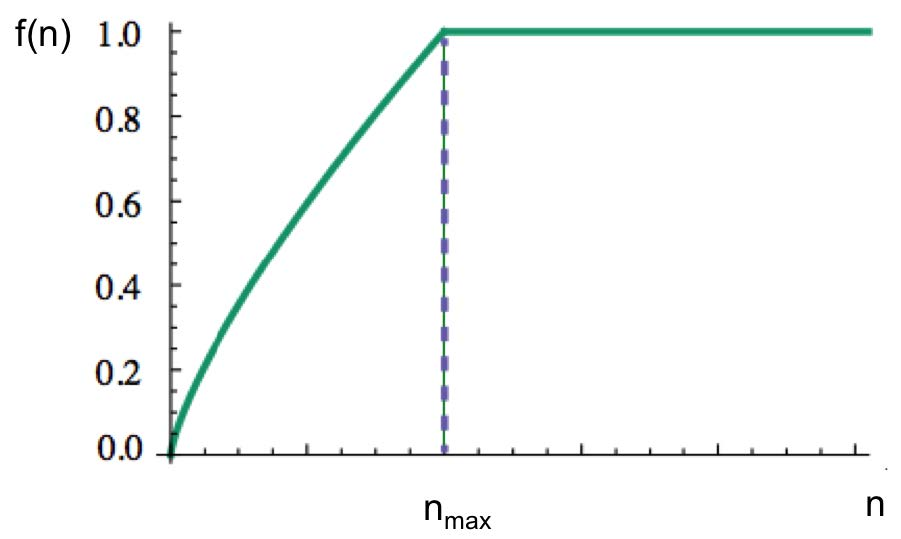
\includegraphics[width=5cm]{fig_5_4.jpg} 
	\caption{The plot of weighting function $f(n)$.}\label{fig_5_4}
\end{figure}
\subsection{Interlude: Normalized vs. Unnormalized Models}
\par At this point, it is worth comparing normalized models and unnormalized ones in a more general view. A normalized model in general over state space $\Omega$ takes the form of
\begin{equation*}
	p(w)=\frac{\exp[h(w)]}{\sum_{w'\in \Omega}\exp[h(w')]}
\end{equation*}
and requires computation of the partition function. The log-likelihood is given by
\begin{equation*}
	\mathcal{L}=\sum_{t}\log p(w_t)
\end{equation*}
and we have
\begin{equation*}
	h(w)\uparrow\ \Longrightarrow p(w)\uparrow\ \Longrightarrow \log p(w)\uparrow\ \Longrightarrow \mathcal{L}\uparrow,
\end{equation*}
which is counterbalanced by normalization: we cannot naively make $h(w)$ large for every $w$ in order to maximize $\mathcal{L}$.
\par An unnormalized model in general, on the other hand, usually take the form of
\begin{equation*}
	\tilde{p}_{\theta}(w)=\exp[h(w)]
\end{equation*}
where the exponential forces non-negativity, and no computation of partition function is required. For unnormalized models, two-sided loss functions are frequently used to make $\tilde{p}_{\theta}(w)$ neither too large nor too small. For example, GloVe uses quadratic loss with log-counts as targets.
\subsection{GloVe Optimization}
First we show that the optimization of GloVe can be regarded as a (weighted) matrix Decomposition task. Without loss of generality, we absorb bias into vectors by letting
\begin{equation*}
	x_{w,d-1}=1,\ x_{w,d}=b_w\ {\rm and}\ y_{w,d-1}=c_w,\ y_{w,d}=1.
\end{equation*}
\begin{remark}\label{rmk_5_constraints}
	In the following discussion from the slides also during the lecture, after using a matrix notation, the constraint on the $(d-1)$-th dimension of ${\bf x}_w$ and the $d$-th dimension of ${\bf y}_w$ are ignored. Like in (\ref{eq_5_mf_prob}), the minimization is taken over ${\bf X,Y}$ without explicit constraints. One possible explanation is the constraints are made implicitly, but this contradicts the argument of ``go beyond SVD'' in the slide. 
\end{remark}
Then we can write everything in matrix forms by defining
\begin{align*}
	&{\bf M}=(m_ij),\ m_{ij}:=\log n_{ij}\\
	&{\bf X}:=[{\bf x}_{w_1}\cdots{\bf x}_{w_{|\mathcal{V}|}}],\ {\bf Y}:=[{\bf y}_{w_1}\cdots {\bf y}_{w_{|\mathcal{C}|}}].
\end{align*}
We therefore see that for GloVe with $f:=1$, optimizing the objective (\ref{eq_5_glv_obj}) is equivalent to solving a matrix factorization problem:
\begin{equation}\label{eq_5_mf_prob}
	\min_{\bf X,Y}\|{\bf M}-{\bf X}^T{\bf Y}\|^2_F
\end{equation}
whose optimal solution is given by (if without the extra constraints, see remark \ref{rmk_5_constraints}) Eckart-Young Theorem (\ref{thm_1_EY}) via SVD noting that the form ${\bf X}^T{\bf Y}$ implies a rank constraint implicitly. However, for a general fixed weight for each entry, we need to go beyond SVD, and this corresponds to solve a matrix factorization problem with a weighted Frobenius norm (Definition \ref{def_3_wtd_f_norm}), and is known to be hard in general. However, for GloVe with weighting function 
\begin{equation*}
	f(n_{ij}):=\begin{cases}
	1 & {\rm if}\ n_{ij}>0,\\
	0 & {\rm otherwise}.
	\end{cases}
\end{equation*}
solves a matrix completion problem
\begin{equation*}
	\min_{\bf X,Y} \sum_{i,j:n_{ij}>0} (m_{ij}-({\bf X}^T{\bf Y})_{ij})^2
\end{equation*}
which falls into a very similar setting we have discussed in section \ref{sec_3_alg_for_mc}, and all the methods like alternating least squares can be applied here.
\par For a general setting of GloVe, the non-convexity makes it hard to find the global minimal, and methods like gradient descent are often used to find a solution. Specifically, for gradient descent (aka steepest descent), we apply the following updating rules until convergence:
\begin{equation*}
	\theta^{\rm new}\leftarrow \theta^{\rm old}-\eta \nabla_{\theta}\mathcal{H}(\theta;{\bf N}),\ \eta>0\ (\text{step size})
\end{equation*}
where $\mathcal{H}(\theta;{\bf N})$ is the GloVe objective function given by (\ref{eq_5_glv_obj}), and 
\begin{equation*}
	\theta=(({\bf x}_w)_{w\in \mathcal{V}},({\bf y}_w)_{w\in \mathcal{C}})
\end{equation*}
are model parameters, i.e. embeddings. However, since the full gradient is often too expensive to compute for a single update, stochastic optimization is more commonly used. For stochastic gradient descent (SGD), we sample $(i,j)$ such that $n_{ij}>0$ uniformly at random, and we perform a "cheap" update for ${\bf x}_i$ and ${\bf y}_j$ with
\begin{align*}
	{\bf x}^{\rm new}_i &\leftarrow {\bf x}_i + 2\eta f(n_{ij})(\log n_{ij}-\langle {\bf x}_i,{\bf y}_j \rangle){\bf y}_j\\
	{\bf y}^{\rm new}_j &\leftarrow {\bf y}_j + 2\eta f(n_{ij})(\log n_{ij}-\langle {\bf x}_i,{\bf y}_j \rangle){\bf x}_i.
\end{align*}
\begin{remark}
	Again we see that there are no explicit constraints on the updates to ensure $x_{w,d-1}=1$ and $y_{w,d}=1$. A possible remedy is applying projected gradient descent instead to force the constraints.
\end{remark}
\section{Word embeddings}
The word embeddings found by distributional context models like skip-gram model turn out to capture semantics of words as expected. For example, the nearest words to "frog" in the embedding vector space are actually frogs, as illustrated in Figure \ref{fig_5_5}, which is remarkable since the model even do not know what a frog looks like.
\begin{figure}[h] 
	\centering 
	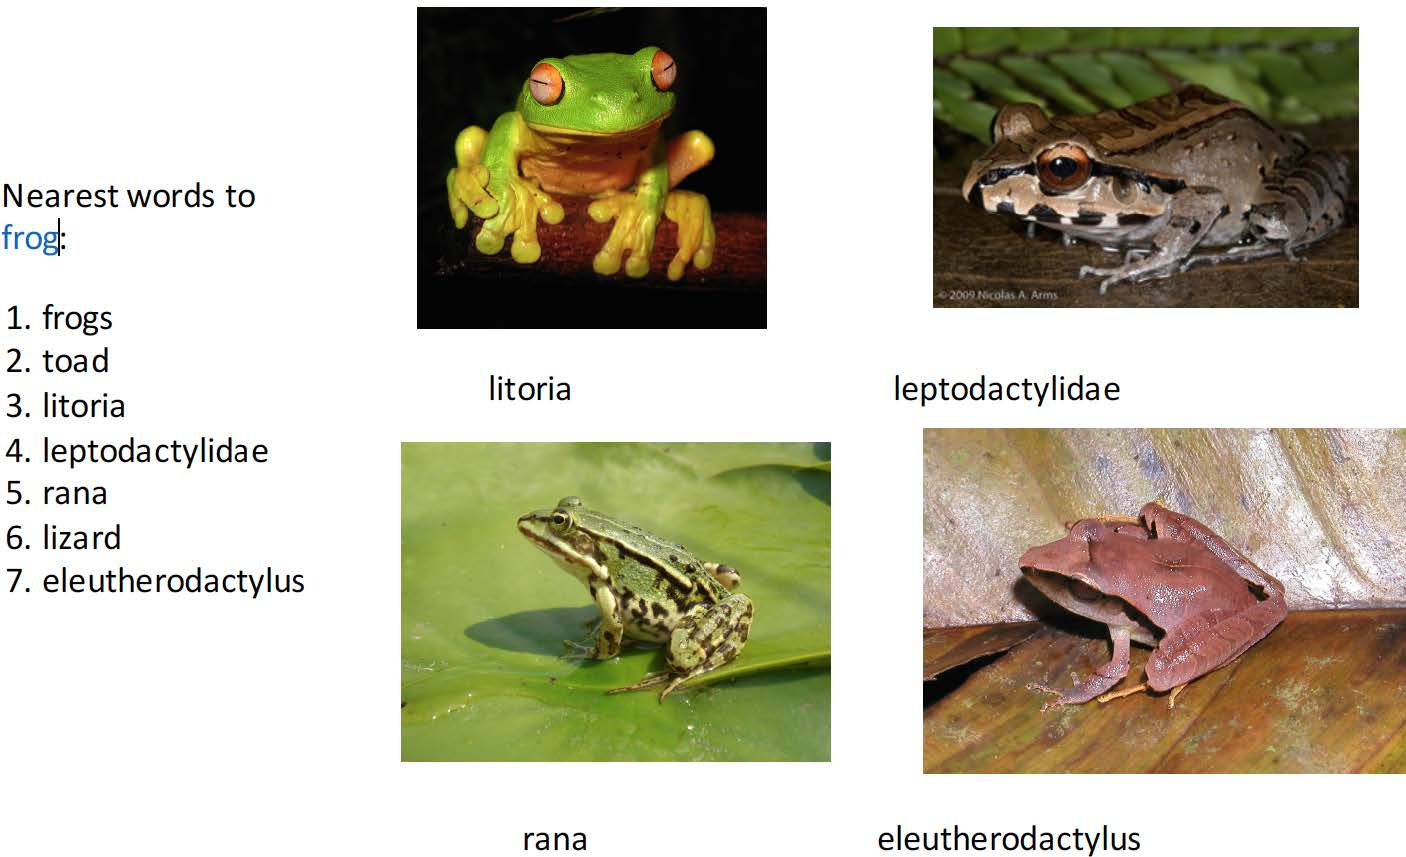
\includegraphics[width=10cm]{fig_5_5.jpg} 
	\caption{The nearest words to "frog" in embedding space.}\label{fig_5_5}
\end{figure}
\par Another interesting property of word embeddings is that it has an affine structure which captures analogies and relatedness. Think of a $a:b::c:?$ type problem, where we need to find a word $d$ that plays a similar role to $c$ as $a$ to $b$. For example, for man:woman::king:? the word "queen" will be a reasonable candidate for $d$. We see that, a model solves this type of problem captures word analogies. Mikolov et al. (2013) proposed that simple algebraic operations could be applied to embeddings to find an analogy prediction. Let ${\bf x}_a$ be the vector for $a$ and so on. For the $d$ such that the analogy holds, we expect
\begin{equation*}
	{\bf x}_b - {\bf x}_a \approx {\bf x}_d-{\bf x}_c.
\end{equation*}
We can find such $d$ by searching in the vector space for the word closest to ${\bf x}_b-{\bf x}_a+{\bf x}_c$ measured by cosine distance. Specifically, we have
\begin{equation*}
	d= \mathop{\arg\max}_{i\in \mathcal{V}\backslash\{a,b,c\}} \cos({\bf x}_i, {\bf x}_b-{\bf x}_a+{\bf x}_c) =\mathop{\arg\max}_{i\in \mathcal{V}\backslash\{a,b,c\}}\frac{({\bf x}_b-{\bf x}_a+{\bf x}_c)^T{\bf x}_i}{\|{\bf x}_b-{\bf x}_a+{\bf x}_c\|}
\end{equation*}
where the second equality holds for normalized word embeddings. Figure \ref{fig_5_6} shows a 2-d projected visualization for analogous word pairs found by word embeddings. We see that, the word embeddings capture the relatedness of man to woman quite well. However, the antonyms ("cheap" vs. "expensive") are usually not well captured.
\begin{figure}[h] 
	\centering 
	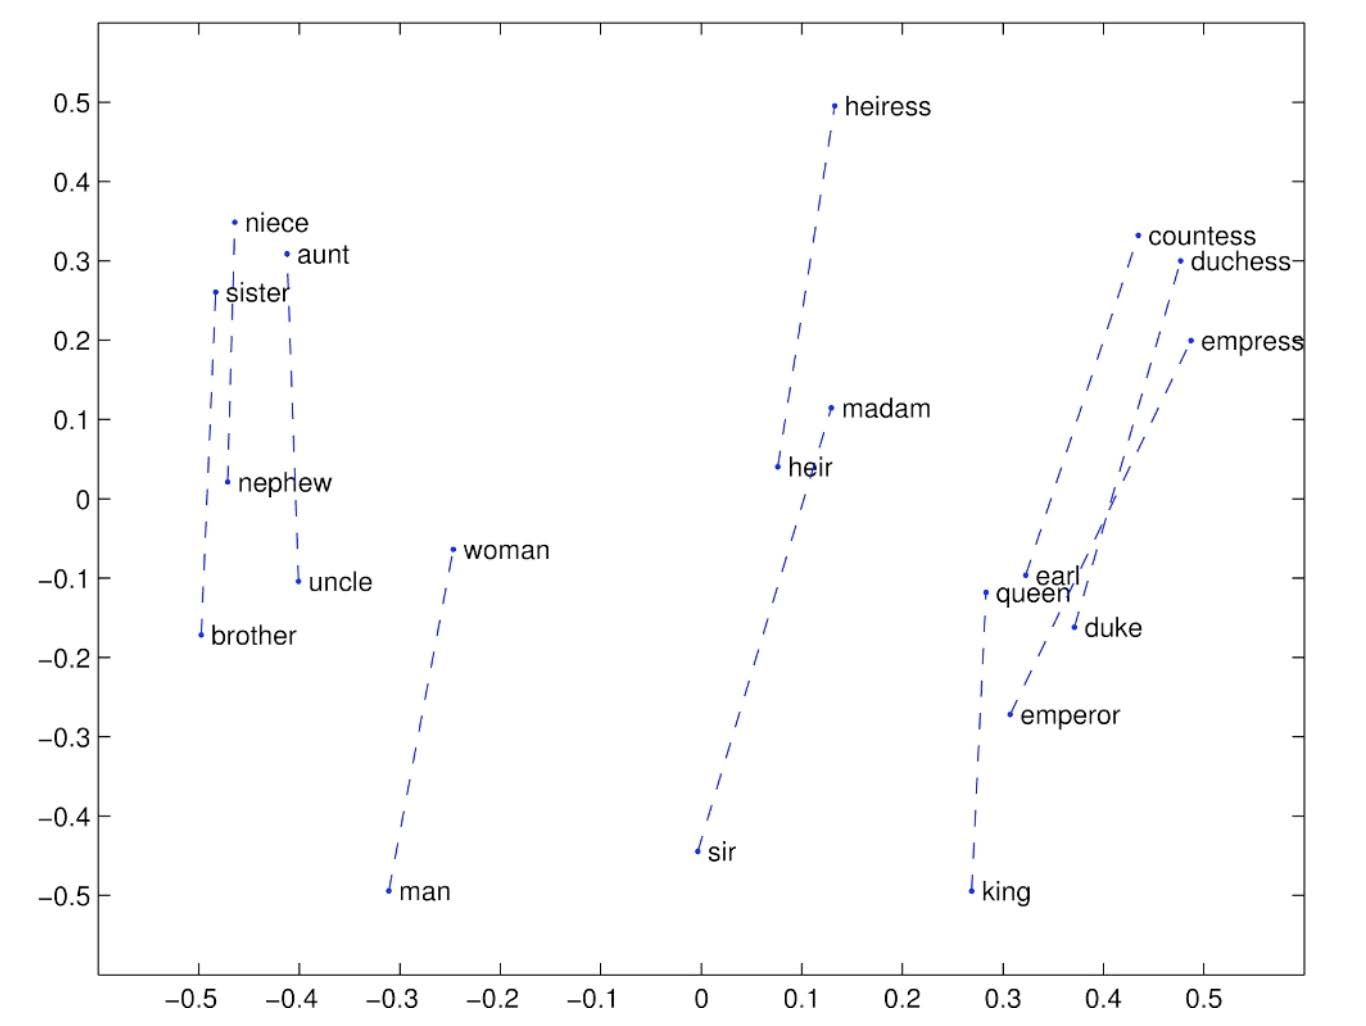
\includegraphics[width=8cm]{fig_5_6.jpg} 
	\caption{2-d projection for word vector analogies found by optimizing the cosine distance for word embeddings.}\label{fig_5_6}
\end{figure}
\par The last thing to discuss of word embeddings is the similar structures of different natural languages. The structures of human languages turn out to be quite similar up to orthogonal transformations (OT) (recall that the methods we have proposed can only find solutions that are unique up to OT since the inner products are invariant under OT). For two languages, if we have some word pairs each of which are of the same meaning, we can then use the embeddings of these pairs to do embedding alignment with orthogonal transformations after which we have words with the same meaning correspond to the same (or close) embedding. People have found that, after alignment, unobserved words with the close meanings also have similar embeddings, which is a remarkable result for machine translation. This suggests also an easy way of creating multilingual embedding space.
\par It is worth mentioning that the idea of word embeddings can also been generalized to sentence or document embeddings. It need more sophisticated analysis and methods like convolutional or recurrent neural network, but is out of the scope of this course.
\begin{figure}[h] 
	\centering 
	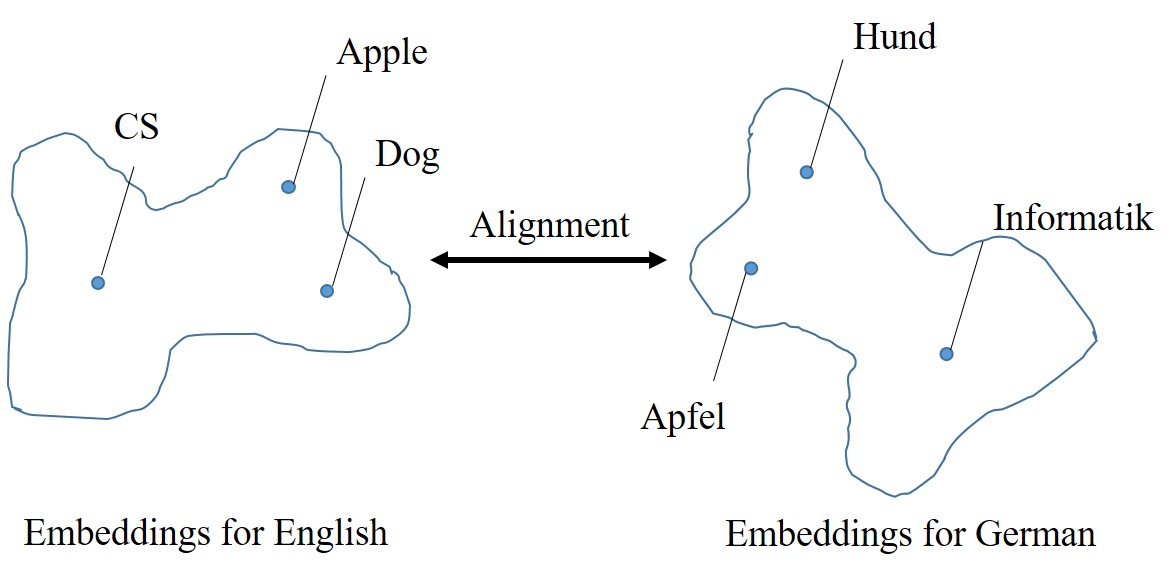
\includegraphics[width=10cm]{fig_5_7.jpg} 
	\caption{Embedding alignment for human languages}\label{fig_5_7}
\end{figure}
%%%%%%%%%%%%%%%%%%%%%%%%%%%%%%%%%%%%%%%%%%%%%%%%%%%%%%%
%   New Chapter                                       %
%%%%%%%%%%%%%%%%%%%%%%%%%%%%%%%%%%%%%%%%%%%%%%%%%%%%%%%

\chapter{Data Clustering and Mixture Models}

%\begin{chapquote}{Author's name, \textit{Source of this quote}}
%``This is a quote and I don't know who said this.''
%\end{chapquote}
In section \ref{sec_4_EM}, we discussed K-means and (Gaussian) mixture models in order to motivate the EM algorithm, while in this chapter we revisit these methods from a view of data clustering. Most of the basic ideas have already been covered in section \ref{sec_4_EM}, and we recommend readers who are interested in more detailed analysis to go through section \ref{sec_4_EM}. Despite the overlapping of the content, in this chapter we will see some recent extensions for K-means to give better guarantees of the performance and handle large data set. We will also briefly discuss about classical model selection methods.
\section{Motivation}
In previous chapters, we have discussed various methods of data reduction, such as PCA and linear autoencoders. Data clustering, however, provide us a different way to look at the reduction problem. Think about a user analysis problem, where we have data of thousands of users and want to extract some useful information. A natural idea is to group similar users together and represent these users with some representative properties, which can be regarded as the features of a prototype associated with this group. Note that with this representation, data compressing is done at the same time. 
\par In general, given a set of data points ${\bf x}_1,\dots, {\bf x}_N\in \mathbb{R}^D$, the goal of data clustering is to find a meaningful partition of the data, i.e. an assignment of each data point to a cluster
\begin{equation*}
	\pi : \{1,\dots,N\}\rightarrow \{1,\dots,K\}
\end{equation*}
or equivalently a partition of the whole data space
\begin{equation*}
	\pi: \mathbb{R}^{D}\rightarrow \{1,\dots,K\}
\end{equation*}
where $K$ is the number of cluster and can be quite arbitrary. We can also recover the $j^{\rm th}$ cluster by
\begin{equation*}
	\pi^{-1}(j)\in\{1,\dots,N\}\text{ or }\in \mathbb{R}^D.
\end{equation*}
Note that $\pi^{-1}(j)$ may not be a function since it maps a number to a set or region. As suggested before, we cluster points via some "similarities" that might help to uncover the hidden group structure of the data, and we can also learning a data density with proper methods. As an example, with the Euclidean distance as the similarity measure and clusters represented by centroids ${\bf u}_j\in\mathbb{R}^D$, we can partition the space $\mathbb{R}^D$ by a mapping induced via a nearest centroid rule
\begin{equation*}
	\pi({\bf x}) = \mathop{\arg\min}_{j=1,\dots,K}\|{\bf u}_j-{\bf x}\|.
\end{equation*}
As illustrated in Figure \ref{fig_6_1}, known as the Voronoi (or Dirichlet) tessellation of $\mathbb{R}^D$, this forms the main idea of \emph{Vector Quantization}.
\begin{figure}[h] 
	\centering 
	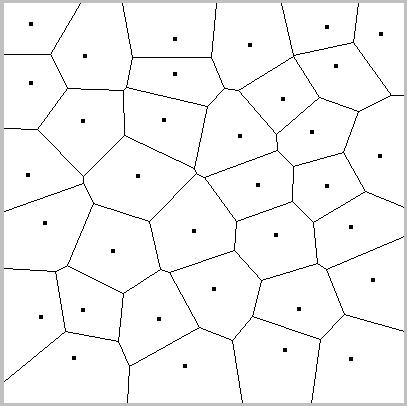
\includegraphics[width=4cm]{fig_6_1.jpg} 
	\caption{An example of Voronoi (or Dirichlet) tessellation, where we see a line connecting 2 points (centroids) will across orthogonally the boundary between the 2 points as implied by the nearest centroid rule.}\label{fig_6_1}
\end{figure}
\section{K-means}
\subsection{Basic Model}
K-means, as one of the most basic algorithm developed in 50s, formalizes the clustering problem as an optimization problem, where we aim to find centroids ${\bf u}_j\in\mathbb{R}^D$ and assignment $\pi$ that minimize a loss function or distortion, e.g. squared Euclidean norm. Concretely, we encode $\pi$ via an indicator matrix ${\bf Z}\in \{0,1\}^{N\times K}$, such that
\begin{equation*}
	z_{ij}:=\begin{cases}
	1&\text{if }\pi({\bf x}_i)=j\\
	0&\text{otherwise}
	\end{cases}.
\end{equation*}
Note that we have
\begin{equation*}
	\sum_{j=1}^{K} z_{ij} = 1,\ \forall i.
\end{equation*}
The K-means objective function measures the distortion of replacing each data point by the assigned centroid and thus takes the form of
\begin{align}
	\label{eq_6_km_obj}J({\bf U, Z})&=\sum_{i=1}^{N}\sum_{j=1}^{K} z_{ij}{\rm dist}({\bf x}_i, {\bf u}_j)=\sum_{i=1}^{N}\sum_{j=1}^{K} z_{ij}\|{\bf x}_i-{\bf u}_j\|^2\\
	\label{eq_6_km_obj_mat}&=\|{\bf X-UZ}^T\|^2_F
\end{align}
where
\begin{align*}
	&{\bf X} = [{\bf x}_1,\dots,{\bf x}_N]\in \mathbb{R}^{D\times N}\ \text{is the data matrix}\\
	&{\bf U} = [{\bf u}_1,\dots,{\bf u}_K]\in \mathbb{R}^{D\times K}\ \text{is the centroid matrix.}
\end{align*}
We see that (\ref{eq_6_km_obj_mat}) is a matrix form of the original K-means objective function (\ref{eq_6_km_obj}) and is followed by
\begin{equation*}
	(\ref{eq_6_km_obj}) = \sum_{i=1}^{N}\left\|{\bf x}_i-\sum_{j=1}^{K} z_{ij}{\bf u}_j\right\|^2 =  \sum_{i=1}^{N}\left\|{\bf x}_i-({\bf UZ}^T)_i\right\|^2 =(\ref{eq_6_km_obj_mat}).
\end{equation*}
The matrix form objective function (\ref{eq_6_km_obj_mat}) shows that K-means solves a matrix decomposition problem, where again we have a rank constraint that is introduced by $K$, and ${\bf Z}$ is not a real value matrix but a selection matrix with $z_{ij}\in\{0,1\}$.
\par As mentioned in section \ref{sec_4_EM}, directly minimizing the K-means objective (\ref{eq_6_km_obj}) is NP-hard, but we still have the following observations:
\begin{itemize}
	\item determining optimal centroids given assignments is easy (continuous variables)
	\item determining optimal assignments given centroids is easy (integer variables).
\end{itemize}
These two simple observations suggest an alternating minimization, i.e. the Lloyd's algorithm in section \ref{sec_4_EM}. Specifically, we alternatively
\begin{itemize}
	\item compute optimal assignment ${\bf Z}$, given centroids ${\bf U}$, by mapping each data point to the closest centroid since each data point contributes to exactly one term in the outer sum of objective (\ref{eq_6_km_obj})
	\begin{equation*}
		z_{ij}^*=\begin{cases}
		1&\text{if }j=\arg\min_k\|{\bf x}_i-{\bf u}_k\|^2\\
		0&\text{otherwise}
		\end{cases}
	\end{equation*}
	\item compute optimal choice of ${\bf U}$, given assignments ${\bf Z}$, by 1st order optimality condition, for non-empty clusters $(\sum_{i=1}^{N}z_{ij}\geq 1)$:
	\begin{equation*}
		\nabla_{{\bf u}_j}J({\bf U,Z})=\sum_{i=1}^{N}z_{ij}\nabla_{{\bf u}_j}\|{\bf x}_i-{\bf u}_j\|^2\overset{!}{=}0\Rightarrow {\bf u}_j^* =\frac{\sum_{i=1}^{N}z_{ij} {\bf x}_i}{\sum_{i=1}^{N}z_{ij}}
	\end{equation*}
	which is known as the centroid condition (center of mass of assigned data points).
\end{itemize}
We can initialize the centroids on $K$ distinct random data points (different initialization may be applied as well) and repeatedly do the above steps until the assignment does not change. With a consistent way to break the ties, where points have equal distances to multiple centroids, K-means algorithm will converge since the objective decrease monotonically, and the number of different assignment is large but finite. Note that the number of step of K-means algorithm until convergence can be very large for extreme cases. Since sometimes during the alternating optimization some clusters become empty, we can do random re-initialization to avoid this problem.
\begin{remark}
	The initialization of K-means can sometimes be problematic. Thinking about the example shown in Figure \ref{fig_6_2}, we see that with the illustrated initialization the final partition might have no cluster taking care of the points on the left. However, it is believed that with a "proper" initialization, K-means will perform well. We will also see more recent extensions of K-means that can handle these problematic cases in the following sections.
	 \begin{figure}[h] 
	 	\centering 
	 	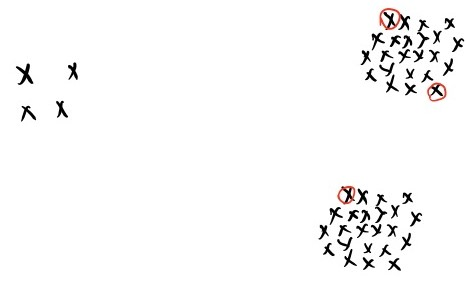
\includegraphics[width=5cm]{fig_6_2.jpg} 
	 	\caption{An example showing that sometimes the initialization will be problematic for K-means. Since there is no initial centroids in the left group, and there are far more points on the right, the final centroids will probably still be around the two groups to the right.}\label{fig_6_2}
	 \end{figure}
\end{remark}
\par The computational cost of each iteration (2 steps) is $O(knd)$. Note that the number of step towards convergence can be very large, so the K-means algorithm can be quite expensive in the worst case. However, as mention before, K-means is guaranteed to converge. Although, the solution might not be global optimal since K-means optimizes a non-convex objective.
\begin{figure}[t] 
	\centering 
	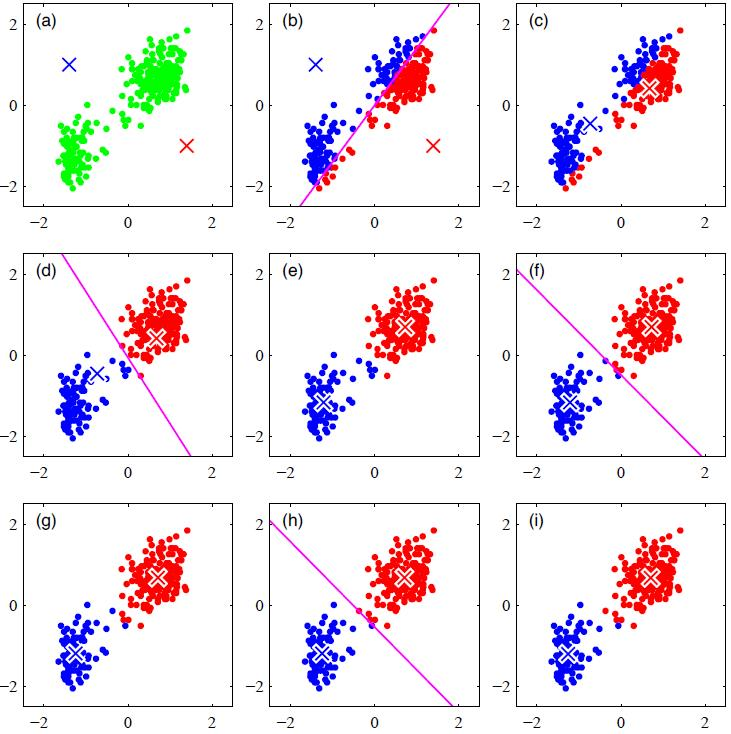
\includegraphics[width=7cm]{fig_6_3.jpg} 
	\caption{Illustration of the K-means algorithm. (Bishop 2006)}\label{fig_6_3}
\end{figure}
\subsection{K-mean++}
K-means++ suggests a more sophisticated seeding for initialization, which was introduced by Arthur \& Vassilvitskii, 2007 and has become a standard extension for K-means for really large data set. Recall that the failure case of random initialization for K-means shows that K-means may stuck at the beginning with at bad initialization. To remedy this, K-means++ suggests an \emph{incremental} $D^2$ (distance square) \emph{sampling} consisting of the following steps
\begin{itemize}
	\item Starting with an initial centroid set $\mathcal{U}_1=\{{\bf x}_I\}$, $I\sim {\rm Uniform}[1:N].$
	\item For $k=1,\dots,K-1$
	\begin{align*}
		&D_i:=\min_{{\bf u}\in \mathcal{U}_k}\|{\bf x}_i-{\bf u}\|,\quad \mathcal{U}_{k+1}:=\mathcal{U}_{k}\cup \{{\bf x}_i\},\ \text{where}\\
		&I\sim {\rm Categorical}({\bf p}),\quad p_i:=\frac{D_i^2}{\sum_{i=1}^{N}D_i^2}.
	\end{align*}
	Here in each step $k$, we construct a distribution according to the centroids that we have sampled, where points that are far from all sampled centroids will have large probabilities. Also, for the points that has been selected as a centroid it has $p_i=0$ since $D_i=0$, which makes sure that there will be no duplicated selection.
\end{itemize}
This sampling method is more expensive (can be implemented in a paralleled way for efficiency) than do thing all randomly, but gives consistently better experimental results. It has been proved that, K-means gives a theoretical guarantee: $O(\log K)$-competitiveness in expectation. Specifically, compared with the optimal clustering, K-means++ gives a solution that might be off by a $O(\log K)$ factor in terms of, say, sum of distortions in expectation. Although the $O(\log K)$ might not be so favorable, it avoids cases that K-means can be arbitrarily bad or fails completely.
\subsection{Core Set for K-means}
K-means++ provides a proper initialization, but K-means algorithm is still computationally expensive for very large data set. Imagine that we have 100 million users, and the question is do we really need so many data to identify groups? An intuitive idea is: maybe the analysis on properly-chosen 100 thousand users is enough to extrapolate the whole data set. However, can we do better to construct the subset than just do random sampling. This is exactly the question that the core set method for K-means aims to answer. The core set approach constructs a weighted sub-data-set on which we can run algorithms like K-means, and by construction we get guarantees of what holds for the large data set. This is a quite recent results by Bachem, Lucic, Krause, 2018: Scalable k-Means Clustering via Lightweight Coresets.
\par Mathematically speaking, K-means aims to find a set $\mathcal{U}$ of $k$ cluster centers in $\mathbb{R}^D$ such that the quantization error $\phi_{\mathcal{X}}(\mathcal{U})$ is minimize, where
\begin{equation}\label{eq_6_qe}
	\phi_{\mathcal{X}}(\mathcal{U}) = \sum_{{\bf x}\in \mathcal{X}}{\rm d}({\bf x}, \mathcal{U})^2=\sum_{{\bf x} \in \mathcal{X}}\min_{{\bf u}\in \mathcal{U}} \|{\bf x-u}\|^2.
\end{equation}
For a weighted set $\mathcal{C}$ with corresponding weights ${\bf w}$, the quantization error is defined as
\begin{equation*}
	\phi_{\mathcal{C}}(\mathcal{U}) = \sum_{{\bf x}\in \mathcal{C}}{\bf w}({\bf x}){\rm d}({\bf x},\mathcal{U})^2.
\end{equation*}
It is proved that, with the following way of sampling the core set, we have
\begin{equation}\label{eq_6_epsi_gua}
	|\phi_{\mathcal{C}}(\mathcal{U}) - \phi_{\mathcal{X}}(\mathcal{U})|\leq \epsilon \phi_{\mathcal{X}}(\mathcal{U})
\end{equation}
with high probability for any $U \subset \mathbb{R}^D$. This shows that we have a control of the performance of K-means on the whole data set.
\par Concretely, we sample the core set, which can be a multi-set (with entries appears multiple times), of size $m$ in the following way. Note that different from K-means++, this is not initialization but sub-sampling data into a smaller set. We sample the core set from
\begin{equation*}
	I\sim {\rm Categ}({\bf p}),\quad p_i:=\frac{1}{2N}+\frac{D_i^2}{2\sum_{j=1}^N D_j^2},\quad D_i^2=\|{\bf x}_i-\mu\|^2
\end{equation*}
where $\mu:=\frac{1}{N}\sum_i {\bf x}_i$ and each sample has a relative weight $\frac{1}{mp_i}$. The probability $p_i$ consists of 2 parts: the first component is the uniform distribution that ensures positivity; the second component is from the intuition that points which are far from the mean of the data have a potentially large impact on the quantization error (\ref{eq_6_qe}) of a clustering. The 2nd component ensures that these potentially important points are sampled frequently enough. As illustrated in Figure \ref{fig_6_4}, the proposed distribution makes points in the small group more likely to be selected.
\begin{figure}[t] 
	\centering 
	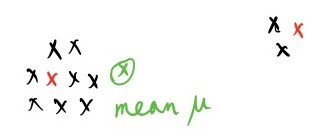
\includegraphics[width=5cm]{fig_6_4.jpg} 
	\caption{Illustration of the core set for K-means algorithm. All data points are represented as a cross with two red ones picked as members of the core set. The mean of the data is represented by the green cross in the circle. The way of sampling make sure that points that are far from the mean have greater probabilities, and the weights $\frac{1}{mp_i}$ compensate for low probabilities of important points near the mean.}\label{fig_6_4}
\end{figure}
\par To explain the role of the weights, we can again take a look at Figure \ref{fig_6_4}, where we have 2 points selected to form the core set. The points close to $\mu$ are with larger quantity but low probabilities, while points that are far from $\mu$ should be fewer but more likely to be chosen. As a result, we have one point from the larger group and one from the smaller cluster. Intuitively, if we want to recover the clustering property of the original data set, we should assign larger weights to the point that are close to $\mu$ to correct for the low probability in selection. The term $m$ in $\frac{1}{mp_i}$ is introduced to make the quantization error of the core set $\phi_{\mathcal{C}}(\mathcal{U})$ an unbiased estimator of the quantization error of the whole data set $\phi_{\mathcal{X}}(\mathcal{U})$. This can be justified by noting that
\begin{equation*}
	\phi_{\mathcal{X}}(\mathcal{U}) = \sum_{{\bf x}\in \mathcal{X}}{\rm d}({\bf x}, \mathcal{U})^2 = \sum_{{\bf x}\in \mathcal{X}}p({\bf x})\frac{{\rm d}({\bf x}, \mathcal{U})^2}{p({\bf x})} = \mathbb{E}\left[\frac{{\rm d}({\bf x}, \mathcal{U})^2}{p({\bf x})}\right]
\end{equation*}
holds for any positive distribution $p({\bf x})$ over $\mathcal{X}$. The quantization error can hence be approximated by sampling $m$ points from $\mathcal{X}$ using $p({\bf x})$ and assigning them weights inversely proportional to $p({\bf x})$. Then we have an unbiased estimator (empirical expectation via sampling) of the $\phi_{\mathcal{X}}(\mathcal{U})$:
\begin{equation*}
	\frac{1}{m}\sum_{{\bf x}\in \mathcal{C}}\frac{{\rm d}({\bf x},\mathcal{U})^2}{p({\bf x})} =\sum_{{\bf x}\in \mathcal{C}} \frac{1}{mp({\bf x})}{\rm d}({\bf x},\mathcal{U})^2 = \phi_{\mathcal{C}}(\mathcal{U}) \approx  \sum_{{\bf x}\in \mathcal{X}}p({\bf x})\frac{{\rm d}({\bf x}, \mathcal{U})^2}{p({\bf x})} =\phi_{\mathcal{X}}(\mathcal{U}).
\end{equation*}
It is proved that this approach gives $\epsilon$-approximation guarantees (\ref{eq_6_epsi_gua}) with probability at least $1-\delta$ for
\begin{equation*}
	m\propto\frac{dk\log k+\log 1/\delta}{\epsilon^2}
\end{equation*}
which shows that the size of core set $\mathcal{C}$ is almost linear in $k$.
\begin{remark}
	Different from K-means++, in the core set sampling we have $D_i = \|{\bf x}_i-\mu\|$ which depends only on ${\bf x}_i$ and a fixed value $\mu=\frac{1}{N}\sum_i {\bf x}_i$. A natural question arises is that whether the distance to $\mu$ is enough to capture the structural properties of a specific point. The answer is probably that it is worth trying. However, we have to keep in mind that we almost always do not know the "right" thing to do, and the proposed core set method works out well for complete data as well in practice. This might suggest that it is better not to make assumptions that are too complicated.
\end{remark}
\section{Mixture Models}
This is a field in statistics that is closely related to K-means. One way to motivate the idea of mixture models is to go from hard assignments in K-means, where each data is assigned to exactly on cluster, to probabilistic assignments, where we want to assign ${\bf x}_i$ to each cluster $j$ with some probability $z_{ij}$. This leads to generalized or relaxed constraints on the selection matrix ${\bf Z}$ given by
\begin{equation*}
	z_{ij}\in [0,1]\ (\forall i,j),\quad \sum_{j=1}^{K}z_{ij}=1\ (\forall i).
\end{equation*}
To do so, we can model each cluster by a probability distribution, which can be the multivariate normal distribution since it is the simplest choice. Just as a quick reminder, the PDF (probability density function) of univariate Gaussian with mean $\mu$ and variance $\sigma^2$ is defined as
\begin{equation*}
	p(x;\mu,\sigma)=\frac{1}{\sigma\sqrt{2\pi}}\exp\left[-\frac{(x-\mu)^2}{2\sigma^2}\right],
\end{equation*}
and an isotropic multivariate normal distribution with mean $\bm{\mu}$ is given by
\begin{equation*}
	p({\bf x};\bm{\mu},\sigma)=\prod_{i=1}^{D}\frac{1}{\sigma\sqrt{2\pi}}\exp\left[-\frac{(x_i-\mu_i)^2}{2\sigma^2}\right].
\end{equation*}
In a more general setting, a multivariate normal distribution with covariance matrix $\bm{\Sigma}$ takes the form of
\begin{equation*}
	p({\bf x},\bm{\mu},{\bf \Sigma})=\frac{1}{|{\bf \Sigma}|^{\frac{1}{2}}(2\pi)^{\frac{D}{2}}}\exp\left[-\frac{1}{2 }({\bf x}-\bm{\mu})^T{\bf \Sigma}^{-1}({\bf x}-\bm{\mu})\right]
\end{equation*}
where ${\bf \Sigma}$ is symmetric and positive definite. Note that the setting with $\bm{\mu}$ and ${\bf \Sigma}$ is generally difficult to estimate for large $D$ since there are in total $D+\frac{D(D+1)}{2}$ parameters.
\par A finite mixture model is defined as a mixture of $k$ (simple) distribution with some mixing proportions
\begin{equation*}
	p({\bf x};\theta)=\sum_{j=1}^{K}\pi_jp({\bf x};\theta_j),\quad \theta=(\pi,\theta_1,\dots,\theta_K)\in \mathbb{R}^{K+K\times M}
\end{equation*}
where $\theta$ are model parameters, and mixing proportions $\pi \geq 0,\ \sum_{j=1}^{K}\pi_j=1$. The density function of each component is given by $p({\bf x};\theta_j)$ with $\theta_j\in\mathbb{R}^M$. For mixture models for clustering, $\pi_j$ has an interpretation as the relative cluster size for cluster $j$ and serves as the probability for each cluster; the location and "shape" of cluster $j$ take a specific form of $p({\bf x};\theta_j)$. As a special case, for Gaussian mixture models, we have 
\begin{equation*}
	\theta_j=(\underbrace{\bm{\mu}_j}_{\rm location},\underbrace{{\bf \Sigma_j}}_{\rm shape}).
\end{equation*}
A Gaussian mixture model (GMM) hence takes the form of
\begin{equation*}
	p({\bf x};\theta)=\sum_{j=1}^{K}\pi_j p({\bf x};\bm{\mu}_j,{\bf \Sigma}_j).
\end{equation*}
This suggests a two-stage generative model: we can generate a data point as follows
\begin{enumerate}
	\item sample cluster index from categorical distribution $j\sim {\rm Categorical}(\pi)$
	\item given $j$, sample a data point ${\bf x}$ from the $j^{\rm th}$ component $\mathcal{N}(\bm{\mu}_j,{\bf \Sigma}_j)$.
\end{enumerate}
Here cluster index $j$ is a latent variable, and the final outcome ${\bf x}$ is what we actually observed. Mathematically speaking, the goal of probabilistic clustering is to compute posteriors of latent cluster memberships. The following part is discussed in more details in section \ref{sec_4_EM}, for maintaining the complete structure of the notes we will briefly discuss it again here.
\par By explicitly introducing latent variables into generative models, hopefully we can simplify the calculations. Concretely, we attach a assignment variable ${\bf z}$ to each data point ${\bf x}$ to form a generic (or complete) data point $({\bf x,z})$, where
\begin{equation*}
	{\bf z}\in\{0,1\}^{K},\quad \sum_{j=1}^{K}z_j=1.
\end{equation*}
The latent variable ${\bf z}$ obeys a categorical distribution
\begin{equation*}
	\mathcal{P}(z_j=1)=\pi_j\quad {\rm or}\quad p_{\pi}({\bf z}) =\prod_{j=1}^{K}\pi_j^{z_j}.
\end{equation*}
Thus, the joint distribution over $({\bf x, z})$ (\textbf{complete data} distribution) is given by
\begin{equation*}
	p({\bf x,z};\theta) = p({\bf z};\theta)p({\bf x}|{\bf z};\theta) = \prod_{j=1}^{K}\pi_j^{z_j} \prod_{j=1}^{K}p({\bf x};\theta_j)^{z_j} = \prod_{j=1}^{K}[\pi_jp({\bf x};\theta_j)]^{z_j}
\end{equation*}
where we have used that $p({\bf x}|{\bf z};\theta) =\prod_{j=1}^{K}p({\bf x};\theta_j)^{z_j}$. With these probabilities, we can play with the posterior assignments. Note that probabilistically speaking, \emph{data generation} is to generate data points ${\bf x}$ given cluster assignments ${\bf z}$, and data inference is to infer cluster assignment ${\bf z}$ given a specific data point ${\bf x}$. Recall that we can compute the posterior by the Bayes rule
\begin{equation*}
	{\rm posterior}\ p(A|B)=\frac{p(B|A)p(A)}{p(B)}
\end{equation*}
where $p(A)$ is the prior, $p(B|A)$ is the likelihood, and $p(B)$ refers to evidence. The posterior probabilities for assignments is therefore
\begin{equation*}
	\mathbb{P}(z_j=1|{\bf x})=\frac{\mathbb{P}(z_j=1)p({\bf x}|z_j=1)}{\sum_{l=1}^{K}\mathbb{P}(z_l=1)p({\bf x}|z_l=1)}=\frac{\pi_jp({\bf x};\theta_j)}{\sum_{l=1}^{K}\pi_lp({\bf x};\theta_l)}
\end{equation*}
where we have assumed access to parameters $\pi, \{\theta_j=(\bm{\mu}_j,{\bf \Sigma}_j)\}$. Suppose that all the data points are drawn independently. The maximum likelihood estimation (MLE) of mixture models requires to optimize
\begin{equation}\label{eq_6_mixture_mle}
	\hat{\theta} = \mathop{\arg\max}_{\theta} \sum_{i=1}^{N}\log p({\bf x}_i;\theta) = \mathop{\arg\max}_{\theta} \sum_{i=1}^{N}\log \left[\sum_{j=1}^{K} \pi_jp({\bf x}_i;\theta_j)\right].
\end{equation}
However, the summation over $j$ inside the logarithm prevents a analytical closed-form solution. A remedy to this problem is the Expectation Maximization (EM) algorithm, which maximize a lower bound on the log-likelihood based on complete data distribution. Specifically
\begin{align}
	\log p({\bf x;\theta})&=\log \left[\sum_{j=1}^{K} \pi_jp({\bf x};\theta_j)\right]=\log \left[\sum_{j=1}^{K} q_j \frac{\pi_jp({\bf x};\theta_j)}{q_j} \right]\notag\\
	\label{eq_6_em_bd}&\geq \sum_{j=1}^{K}q_j[\log p({\bf x};\theta_j) +\log \pi_j - \log q_j]
\end{align}
where $q_j$ is a distribution over $j=1,\dots,K$, such that $q_j>0,\ \sum_j q_j=1$, and the inequality follows by the Jensen's inequality noting the concavity of logarithm. Note that the summation over $i$ in MLE objective (\ref{eq_6_mixture_mle}) is outside of the logarithm, so we can evaluate the contribution of each data point ${\bf x}_i$ by the proposed lower bound separately (additive).
\par In the expectation step (E-step), we optimized bound (\ref{eq_6_em_bd}) with regard to the distribution $q$. We formulate the following Lagrangian (decoupled for each data point)
\begin{equation*}
	\max_{q}\left\{\sum_{j=1}^{K}q_j[\log p({\bf x};\theta_j) +\log \pi_j - \log q_j] +\lambda (\sum_{j=1}^{K}q_j -1) \right\}.
\end{equation*}
Apply the first order optimality condition (setting gradient to zero) we get:
\begin{align*}
	&\log p({\bf x};\theta_j) +\log \pi_j - \log q_j - 1 +\lambda \overset{!}{=}0 \Longleftrightarrow\\
	&q_j^*=\frac{\pi_jp({\bf x};\theta_j)}{\sum_{l=1}^{K}\pi_lp({\bf x};\theta_l)}\overset{\rm Bayes\ rule}{=}\mathbb{P}(z_j=1|{\bf x})
\end{align*} 
which shows that the optimal $q$-distribution equals to the posterior given the parameters. In another word, E-step selects the best lower bound on the log-likelihood given ${\bf \theta}$.
\par In the maximization step (M-step), we optimize expected complete data log-likelihood with regard to the model parameters. Note that the problem decouples for each cluster and with regard to $\pi$. Specifically, combining the MLE objective (\ref{eq_6_mixture_mle}) and the lower bound for each point (\ref{eq_6_em_bd}), we get
\begin{align}
	\label{eq_6_em_bd_cplt}\sum_{i=1}^{N}\log p({\bf x}_i;\theta) &\geq \sum_{i=1}^{N}\sum_{j=1}^{K}q_{ij}[\log p({\bf x}_i;\theta_j) +\log \pi_j - \log q_{ij}]\\
	&=\sum_{i=1}^{N}\sum_{j=1}^{K}q_{ij}\log p({\bf x}_i|z_{ij}=1;\theta)p(z_j=1) -q_{ij}\log q_{ij}\notag\\
	\label{eq_6_em_bd_ana}&=\sum_{i=1}^{N}\sum_{j=1}^{K}\mathbb{P}(z_j=1|{\bf x}_i)\log p({\bf x}_i,z_j=1;\theta) +{\rm const}
\end{align}
where $q_{ij}$ and $z_{ij}$ are the $q_j$ in (\ref{eq_6_em_bd}) and $z_j$ for ${\bf x}_i$ respectively, and we have assumed fixed $q_{ij} = \mathbb{P}(z_j=1|{\bf x}_i)$; the constant is for that they are only related to $q_{ij}$. If we write the first term of (\ref{eq_6_em_bd_ana}) in a matrix form, we get
\begin{equation*}
	\sum_{\bf Z}\mathbb{P}({\bf Z}|{\bf X})\log p({\bf X,Z};\theta)=\mathbb{E}_{\bf Z|X}\log p({\bf X,Z};\theta)
\end{equation*}
which shows that we are optimizing the expected complete data log-likelihood. Given fixed $q_{ij} = \mathbb{P}(z_j=1|{\bf x}_i)$, we can again apply the first order optimality condition with Lagrangian to solve for optimal $\pi$ and $ \theta_j = (\bm{\mu}_j,\bm{\Sigma}_j)$:
\begin{align*}
	&\nabla_{\pi_j}\left[\sum_{i=1}^{N}\sum_{j=1}^{K}q_{ij}\log \pi_j +\lambda(\sum_{l=1}^{K} \pi_l-1)\right]\overset{!}{=}0\Rightarrow \pi_j^* =\frac{1}{N}\sum_{i=1}^{N}q_{ij}\\
	&\nabla_{\bm{\mu}_j}\sum_{i=1}^{N}\sum_{j=1}^{K}q_{ij}\log \mathcal{N}({\bf x}_i;\bm{\mu}_j,{\bf \Sigma}_j) \overset{!}{=}0\Rightarrow \bm{\mu}_j^*=\frac{\sum_{i=1}^{N}q_{ij}{\bf x}_i}{\sum_{i=1}^{N}q_{ij}}\\
	&\nabla_{\bm{\Sigma}_j}\sum_{i=1}^{N}\sum_{j=1}^{K}q_{ij}\log \mathcal{N}({\bf x}_i;\bm{\mu}_j,{\bf \Sigma}_j) \overset{!}{=}0\Rightarrow \bm{\Sigma}_j^*=\frac{\sum_{i=1}^{N}q_{ij}({\bf x}_i-\bm{\mu}_j)({\bf x}_i-\bm{\mu}_j)^T}{\sum_{i=1}^{N}q_{ij}}.
\end{align*}
Solving the optimal covariance matrix needs some extra tool of matrix derivative, where one might need:
\begin{equation*}
	\frac{\partial}{\partial {\bf A}}\ln |{\bf A}|=({\bf A}^{-1})^T,\ \frac{\partial}{\partial {\bf A}} {\rm Tr}({\bf AB})={\bf B}^T.
\end{equation*}
The EM algorithm works by alternate E-steps and M-steps, and both E and M step are maximizing the same objective. As in K-means, it is guaranteed to converge towards a point $\theta^*$ (with some convergence criteria), while, again like in K-means, $\theta^*$ may not be the global maximizer. As a summary, we have
\begin{itemize}
	\item E-step: compute probabilistic assignments of points to clusters (keeping their location and shape fixed)
	\item M-step: recompute optimal cluster locations and shapes, given probabilistic assignments.
\end{itemize}
\begin{figure}[h] 
	\centering 
	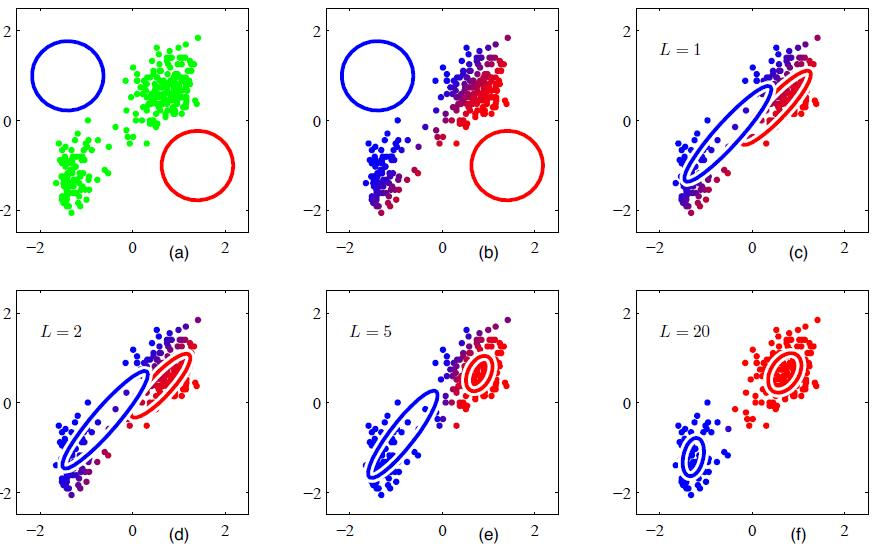
\includegraphics[width=10cm]{fig_6_5.jpg} 
	\caption{Gaussian mixture model fitting via EM for two clusters. Remark: here the covariance is also estimated (illustrated by the two ellipsoids). (Bishop 2006)}\label{fig_6_5}
\end{figure}
To conclude this section, we now spend some time comparing the two clustering algorithms mentioned up to now:
\begin{itemize}
	\item Assignments:
	\begin{itemize}
		\item K-means algorithm: hard assignment points to clusters
		\item EM algorithm: soft assignment based on posteriors
	\end{itemize}
	\item Shapes:
	\begin{itemize}
		\item K-means: spherical cluster shapes, uniform spread
		\item EM: can learn covariance matrix (ellipsoid-shaped)
	\end{itemize}
	\item K-means as a special case: as discussed in section \ref{sec_4_em_km_compare}, K-means can be regarded as a special case of Gaussian mixture models with (fixed) covariance ${\bf \Sigma}_j=\sigma^2{\bf I}$ in the limit of $\sigma \rightarrow 0$ (hard assignment).
\end{itemize}
\par In practice, EM algorithm takes much more iterations to converge and in each cycle requires significantly more computation. In this case, K-means can be used to find a good initialization of the EM: covariance matrices can be initialized to the sample covariances of the clusters found by the K-means algorithm; mixing coefficients can be set to the fractions of data points assigned to the respective clusters.
\section{Model Selection}
The last topic of this chapter is about model selection which is often motivated by this kind of questions: what is the proper number of model parameters, or how should we determine the model complexity? In a typical machine learning task people usually have to find trade-off between two conflicting goals:
\begin{itemize}
	\item Data fit: We want to predict the data well, e.g., maximizing the data log-likelihood. In this case, usually more complex model gives better fit on the observed data.
	\item Complexity: Choose a model that is not very complex which is often measured by the number of free parameters. Too complex models tend to over fit the observed data and give bad generalization power.
\end{itemize}
Take the number of clusters in a data clustering problem as an example. Recall that the negative log-likelihood of data for $K$ mixture Gaussians can be written as
\begin{equation*}
	-\log p({\bf X};\theta)=-\sum_{i=1}^{N}\log \left[\sum_{j=1}^{K}\pi_jp({\bf x}_i;\theta_j)\right].
\end{equation*}
For one specific clustering algorithm like K-means, the negative log-likelihood v.s. number of clusters $K$ usually takes the form as illustrated in Figure \ref{fig_6_6}. Note that smaller negative log-likelihood means better fit (to the observed data). As illustrated, in general the objective decreases with $K$ (some noise due to local minima), but very small does not necessarily mean a good fit. 
\begin{figure}[h] 
	\centering 
	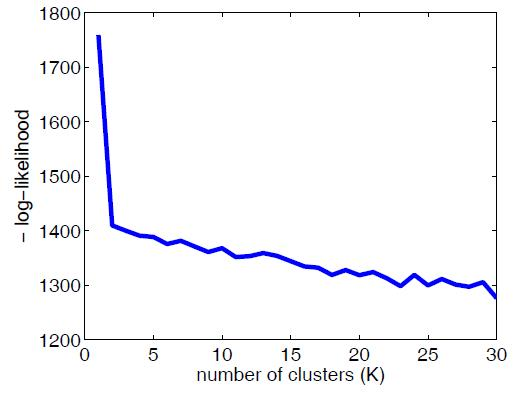
\includegraphics[width=5cm]{fig_6_6.jpg} 
	\caption{A typical negative log-likelihood plot of clustering algorithms}\label{fig_6_6}
\end{figure}
\par If we measure the model complexity by the number of free parameters $\kappa(\cdot)$, there are two heuristics for choosing $K$:
\begin{itemize}
	\item Akaike Information Criterion (AIC):
	\begin{equation*}
		{\rm AIC}(\theta|{\bf X})=-\log p({\bf X};\theta)+\kappa(\theta)
	\end{equation*}
	\item Bayesian information Criterion (BIC):
	\begin{equation*}
		{\rm BIC}(\theta|{\bf X})=-\log p({\bf X};\theta)+\frac{1}{2}\kappa(\theta)\log N
	\end{equation*}
\end{itemize}
Generally speaking, the BIC criterion penalizes complexity more than the AIC criterion. Note that a single AIC (BIC) result is meaningless. One has to repeat the analysis for different $K$ and compare the differences: the most suitable number of clusters corresponds to the smallest AIC (BIC) value. As an example, we can consider a mixture of Gaussians:
\begin{itemize}
	\item Number of free parameters (with fixed covariance matrices) is
	\begin{equation*}
		\kappa(\theta)=\underbrace{K\cdot D}_{\bm{\mu}}+\underbrace{(K-1)}_{\pi}
	\end{equation*}
	\item Number of free parameters (with full covariance matrices) is given by
	\begin{equation*}
	\kappa(\theta)=K\cdot\left(\underbrace{D}_{\bm{\mu}} +\underbrace{\frac{D(D+1)}{2}}_{\bm{\Sigma}} \right)+\underbrace{(K-1)}_{\pi}.
	\end{equation*}
\end{itemize}
Figure \ref{fig_6_7} and Figure \ref{fig_6_8} illustrate AIC and BIC examples for 3 and 5 clusters respectively. We can see that in both case, the minimal values of BIC and AIC value correspond to the "right" number of clusters.
\begin{figure}[h] 
	\centering 
	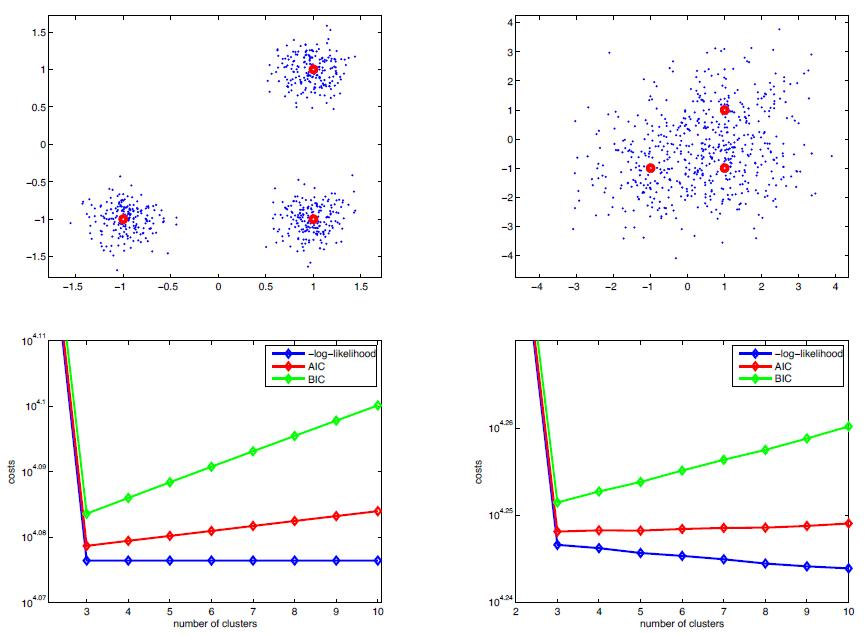
\includegraphics[width=12cm]{fig_6_7.jpg} 
	\caption{Information criteria for a synthetic dataset with 3 clusters. Synthetic data has smaller variance on the left than on the right.}\label{fig_6_7}
\end{figure}
\begin{figure}[h] 
	\centering 
	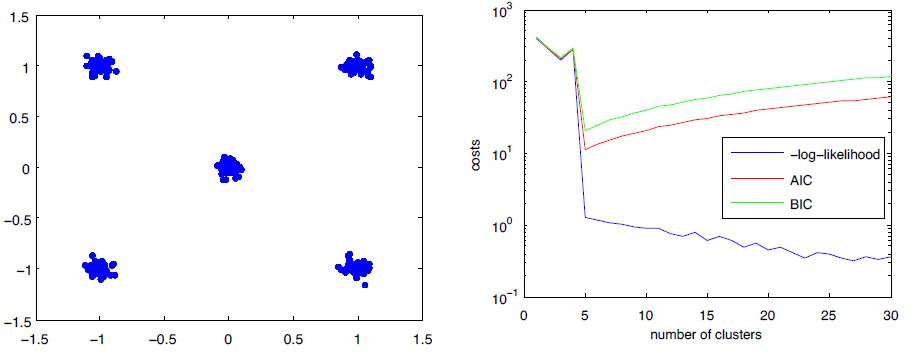
\includegraphics[width=12cm]{fig_6_8.jpg} 
	\caption{Information criteria for a synthetic dataset with 5 clusters.}\label{fig_6_8}
\end{figure}
%%%%%%%%%%%%%%%%%%%%%%%%%%%%%%%%%%%%%%%%%%%%%%%%%%%%%%%
%   New Chapter                                       %
%%%%%%%%%%%%%%%%%%%%%%%%%%%%%%%%%%%%%%%%%%%%%%%%%%%%%%%

\chapter{Neural Networks}
In the previous chapters we met neural networks several times. We now formally introduce the basic ingredients of them and the most well-known algorithm for parameter learning, backpropagation. From several ``modern'' extensions of neural networks in the end of this chapter we will get a glimpse of the modeling power of neural networks. Neural networks have been investigated very early in late 50s and 60s as a model of computation for brains and computers. In the 80s with backpropagation and so on and so forth, neural networks succeeded in few things, and were forgot by the research community until their reemergence in around 2010 when deep learning came into play. We start with a standard model.

\section{Multilayer Perceptrons}
\subsection{An overview}
A neural network can be regard as a function that computes outputs given inputs by connected computational units. These units, also refer to neurons, are parametrized by some adaptable weights that can be learned. Each unit implements only a basic operation: a generalized linear function combined with a non-linear activation function. So to speak, each unit computes a non-linear function consisting of
\begin{equation*}
	{\rm linear\ function}:\ \mathbb{R}^n\rightarrow \mathbb{R}\ +\ \text{non-linear activation function}\ \sigma:\mathbb{R}\rightarrow \mathbb{R},
\end{equation*}
where we use linear functions for their simplicity. The non-linear activation function $\sigma$ is usually fixed and not adaptable. There are several popular choices of $\sigma$, but in a particular neural network people usually only use one type of $\sigma$. The reason to use this kind of combination to encode non-linearity rather than allow any non-linear function is because we want to keep things as simple as possible in terms of each computational unit (recall that we have the flexibility in connecting them). It is also proved that neural nets with fixed simple activation functions can approximate any non-linear function arbitrarily well. Mathematically, each unit is parametrized with weight ${\bf w}\in \mathbb{R}^{n+1}$, and computes
\begin{equation*}
	f^{\sigma}({\bf x},{\bf w}):=\sigma\left(w_0+\sum_{i=1}^{n}w_ix_i\right)=\sigma({\bf w}^T{\bf x})
\end{equation*}
as shown in Figure \ref{fig_7_1}, where in the last equality we ignore or absorb (rewrite ${\bf x}\rightarrow (1,{\bf x})$) bias parameter $w_0$ for clarity.
\begin{figure}[h] 
	\centering 
	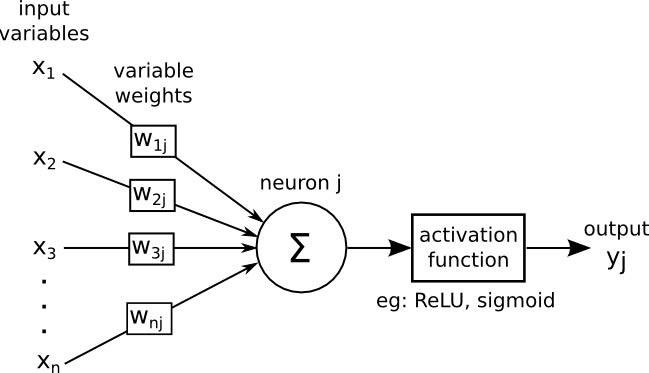
\includegraphics[width=8cm]{fig_7_1.jpg} 
	\caption{A schematic view for a unit in neural networks}\label{fig_7_1}
\end{figure}
\subsection{Activation function}
Despite the arbitrariness of choosing activation functions, there are two types of functions that are mostly used: the old school choice, logistic function (left of Figure \ref{fig_7_2}), and the new school choice, ReLU (rectified linear unit) (right of Figure \ref{fig_7_2}).
\begin{figure}[h] 
	\centering 
	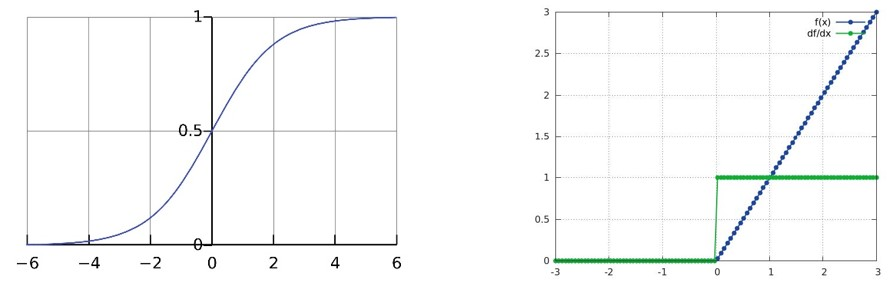
\includegraphics[width=12cm]{fig_7_2.jpg} 
	\caption{Left: logistic function. Right: ReLU.}\label{fig_7_2}
\end{figure}
\par The logistic function (left of Figure \ref{fig_7_2}), also called sigmoid function because of its shape, is given by
\begin{equation*}
	{\rm sigmoid}(x) = \frac{1}{1+\exp(-x)}.
\end{equation*}
Note that it can be regard as the same function as $\tanh$ up to a rescaling and shifting since
\begin{equation*}
	\tanh(x)=\frac{e^{x}-e^{ -x}}{e^{ x}+e^{ -x}} = 2\frac{e^{ x}}{e^{ x}+e^{ -x}} -1=2\frac{1}{1+e^{-2{ x}}} - 1= 2 {\rm sigmoid}(2{ x})-1.
\end{equation*}
\par The logistic function has the property that $x\rightarrow \infty,\sigma(x)\rightarrow 1$ and $x\rightarrow -\infty,\sigma(x)\rightarrow0$. This has a motivation from biology side where this type of saturate effect (maximal level of activity and inactivity) is quite common. Also mathematically speaking, the logistic function is a smooth version of the ``switch'' function, where by smooth it means differentiable up to any order, and thus has many nice mathematical properties.
\par On the other hand, ReLU (right of Figure \ref{fig_7_2}) appears to be a simpler and more straightforward function defined by
\begin{equation*}
	{\rm ReLU}_{\bf w}({\bf x})=\max(0,{\bf w}^T{\bf x}),
\end{equation*}
where as its name rectified linear unit suggests it is a unit parametrized by weight ${\bf w}$. The non-linear activation function of ReLU is just given by $\max(0, x)$. ReLU is a linear function over half-space $\mathcal{H}=\{{\bf x}:{\bf w}^T{\bf x}>0\}$ and zero on its complement $\mathcal{H}^c=\mathbb{R}-\mathcal{H}$. Different from the logistic function, it's non-smooth, but simple derivatives over $\mathbb{R}-\{0\}$. Therefore, to some degree, we can say that the ReLU function has minimal non-linearity.
\subsection{Multilayer Perceptron}
With a model for each unit, we can put these neurons together to form a computational graph where we do this in terms of layers (Figure \ref{fig_7_3}). Although we have the freedom to make (directed) connections quite arbitrarily as long as there's no loop, which is essential for these graphs to be computable, this layer architecture gives a rather simple but still adaptable model enough for exploring. 
\begin{figure}[h] 
	\centering 
	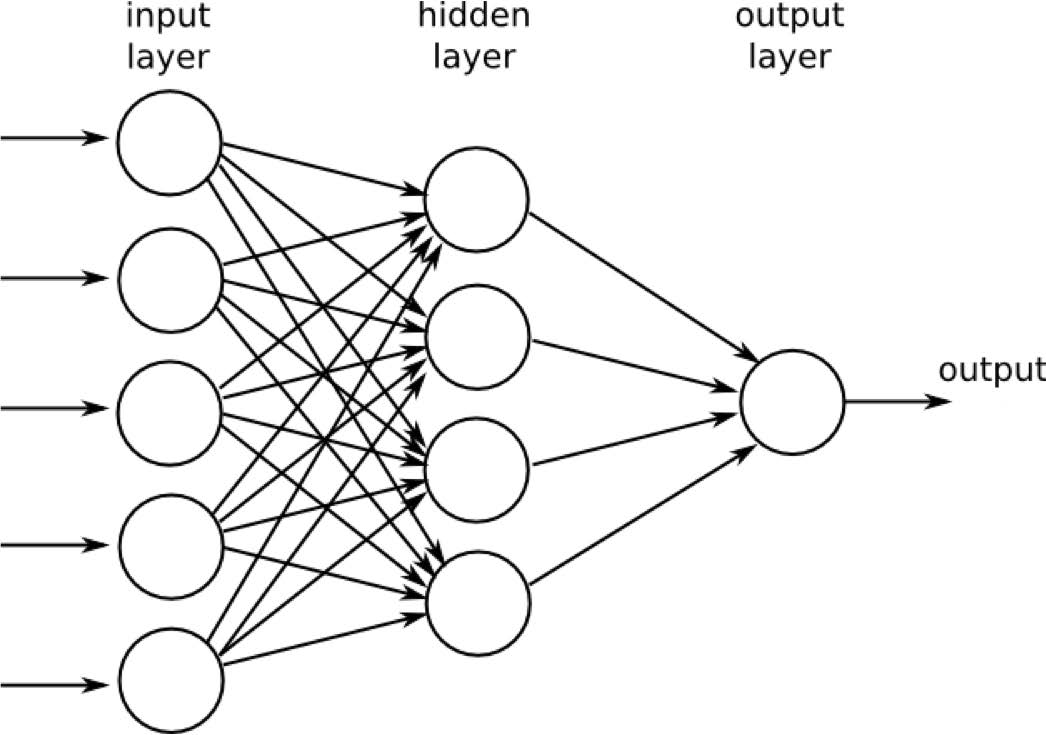
\includegraphics[width=6cm]{fig_7_3.jpg} 
	\caption{A typical structure for neural networks.}\label{fig_7_3}
\end{figure}
\par Typically, the first layer is the raw input ${\bf x}$, where no computation is involved; the last layer serves as the final output whose form depends on specific task (class label for image classification). Although what the input and the output should be is clear in this case, we have no idea about what the intermediate layers represent, and how to learn the weights becomes a big question. To start our discussion, we first build up some useful notations.
\par As mentioned above, we arrange units in layers. With units indexed by $j$ and a shared choice of $\sigma$, we can write the (fully connected) mapping between two layers in a vector form
\begin{equation*}
	F^{\sigma}:\ \mathbb{R}^n\rightarrow \mathbb{R}^m,\ F^{\sigma}_{j}({\bf x})=\sigma({\bf w}_j^T{\bf x}),\ j=1,\dots,m,
\end{equation*}
where $n$ and $m$ represent the number of units of the previous/old and the current/new layer respectively; ${\bf x}$ can be the input or activation of the previous layer, and $ F^{\sigma}_{j}$ denotes a unit in the current layer. We can also take one step further to make everything in a matrix-vector notation ($\sigma$ is applied elementwise):
\begin{equation*}
	F^{\sigma}({\bf x};{\bf W})=\sigma({\bf Wx}),\ {\bf W}=({\bf w}_1,\dots, {\bf w}_m)^T.
\end{equation*}
If we index layers by $l$, the activation vector of $l$-th layer by ${\bf x}^{(l)}$, we get a indexed notation for layer-to-layer forward propagation in the form of
\begin{equation*}
	{\bf x}^{(l)}=\sigma^{(l)}({\bf W}^{(l)}{\bf x}^{(l-1)}),\ {\bf W}^{(l)}\in \mathbb{R}^{n_l\times n_{l-1}},
\end{equation*}
where ${\bf W}^{(l)}$ is the weight matrix between layer $l-1$ and layer $l$; ${\bf x}^{(1)}$ is the input; ${\bf x}^{(L)}$ is the output, and ${\bf x}^{(l)}$ $(1<l<L)$ are the hidden layers. \par With these notations, we can represent a $L$-layer network with a nested function given by
\begin{equation*}
	{\bf y} = \sigma^{(L)}\left({\bf W}^{(L)}\sigma^{(L-1)}\left(\cdots\left({\bf W}^{(2)}\sigma^{(1)}\left({\bf W}^{(1)}{\bf x}^{(1)}\right)\right)\cdots\right)\right).
\end{equation*}
There 2 important degrees of freedom for our layer architecture:
\begin{itemize}
	\item Layer width: a wider layer means ``more of the same'' feature since the units in the same layer have the same input, the activation from the previous layer or the input.
	\item Network depth: different from the layer width, a deeper network allows ``more compositionality'' meaning that the network can have more ability to combine things and thus capture complex things. By using a deep network, we form a feature hierarchy.
\end{itemize}
\par The output layer, as mention before, depends on that type of problem we want to solve, where we may not want to naively apply the same activation function as previous layers. To simplify the notation, we have ${\bf W} = {\bf W}^{(L)},\ {\bf x}={\bf x}^{(L-1)}$. For a linear regression task, it's convenient to simply have a linear activation:
\begin{equation*}
	{\bf y}={\bf Wx}.
\end{equation*}
While for a binary classification task, we want only one output ranging from 0 to 1 to form a valid conditional probability distribution. Then the logistic function can be a reasonable choice:
\begin{equation*}
	y_1 = P(Y=1|{\bf x})=\frac{1}{1+\exp[-{\bf w}^T {\bf x}]}.
\end{equation*}
For the multiclass case with $K$ classes, soft-max function is usually the top choice:
\begin{equation*}
	y_k = P(Y=k|{\bf x})=\frac{\exp[{\bf w}_k^T {\bf x}]}{\sum_{j=1}^{K}\exp[{\bf w}_j^T {\bf x}]}.
\end{equation*}
\par At this point, it is worth spending some time take a look at the multilayer perceptron and logistic regression in terms of classification methods. In logistic regression, we compute a linear function of inputs and map it to $(0,1)$:
\begin{equation*}
	P(Y=1|{\bf x})=\frac{1}{1+\exp[-\langle{\bf w,x}\rangle]},
\end{equation*}
where ${\bf x}$ can be the original input or some learned better representations. While a multilayer perceptron first tries to learn intermediate feature representation and then perform logistic regression on learned representation ${\bf x}^{(L-1)}$. In a word, logistic regression is about: give me good representations I tell you how to linearly separate things, where logistic regression do nothing about the representations. Multilayer perceptron can learn different representations and applies logistic regression to give outputs.
\subsection{Loss Function}
Before we move forward to the learning algorithm, let us first think about what in the model needs to be learned. Things like model architecture (including the number of layers, the number of units in each layer, etc.) and the activation function $\sigma$ are our choices. We desire algorithms to learn the weights, i.e. algorithms that can automatically fiddling with network weights. 
\par The idea is to make the learning problem an optimization problem. To do so, we first need to define a \textbf{loss} function $l(y^*;y)$, where $y^*$ and $y$ are the target output and prediction respectively. Again, the form of loss function depends on the nature of the task. For a regression problem, where $y^*,y\in \mathbb{R}$, we might want to use a squared loss
\begin{equation*}
l(y^*;y)=\frac{1}{2}(y^*-y)^2.
\end{equation*}
For a binary classification task, we might desire the cross-entropy loss
\begin{equation*}
	l(y^*;y)=-y^*\log y-(1-y^*)\log(1-y),
\end{equation*}
where $0\leq y\leq 1$ is used to model a Bernoulli distribution; $y^*\in \{0,1\}$ or $\in [0,1]$ (when $y^*\in [0,1]$ is a real number, this has the interpretation as a soft target encoding the uncertainty about the labeling). There is a close relationship between the cross-entropy loss and the log-likelihood. In general, the cross-entropy $H(p,q)$ measures the difference between distributions $q$ and $p$:
\begin{equation*}
	H(p,q)=-\mathbb{E}_p[\log q]=-\sum_{x\in\mathcal{X}}p(x)\log q(x)\ (\text{discrete case}).
\end{equation*}
For a classification problem, if the predicted probabilities are $q_i$, while the frequency (empirical probability) of $i$ in the training set is $p_i$, and there are $N$ independent samples in the training set, then the likelihood of the training set is
\begin{equation*}
	\prod_{i}(\text{probability of }i)^{\text{number of occurences of }i}=\prod_{i}q_i^{Np_i}.
\end{equation*}
So the log-likelihood, divided by $N$ is
\begin{equation*}
	\frac{1}{N}\log \prod_{i}q_i^{Np_i}=\sum_i p_i\log q_i=-H(p,q).
\end{equation*}
For a single point in a binary classification problem, $p\in \{y^*,1-y^*\}$ and $q\in \{y,1-y\}$, then we have
\begin{equation*}
	H(p,q) = -\sum_i p_i\log q_i=-y^*\log y-(1-y^*)\log(1-y).
\end{equation*}
When we generate $y$ with logistic function, the cross-entropy loss sometimes also refers to negative logistic log-likelihood. 
\begin{figure}[h] 
	\centering 
	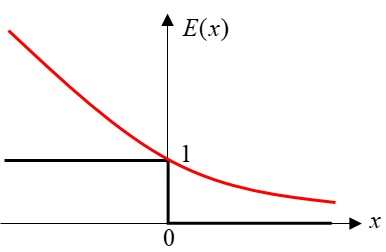
\includegraphics[width=6cm]{fig_7_4.jpg} 
	\caption{The plot of misclassification error (black) and cross-entropy loss (red) for $y^*=1$. The cross-entropy is rescaled by a factor of $1/\ln 2$, so that it pases trough the point $(0,1)$, and $x$ is the input for logistic function, i.e. $y=1/(1+\exp[-x])$.}\label{fig_7_4}
\end{figure}
\par The cross-entropy loss can be regarded as a differentiable approximation or surrogate to the misclassification error as illustrated in Figure \ref{fig_7_4}, and can never reach 0 when logistic function is applied.
\par With a loss function, we can define the objective of the optimization task for parameter learning. Specifically, given a training set of examples $\mathcal{X}-\{({\bf x}_t,y):t=1,\dots,T\}$, we'd like to minimize the empirical risk (average loss on the training data) given by
\begin{equation*}
	\mathcal{L}(\theta;\mathcal{X})=\frac{1}{T}\sum_{t=1}^{T}l(y_t;\underbrace{y({\bf x}_t;\theta)}_{\text{NN output}}),\ \theta=\left({\bf W}^{(1)},\dots,{\bf W}^{(L)}\right).
\end{equation*}
Sometimes people apply regularization to make networks generalize better. Briefly speaking, by adding regularization we add prior knowledge (not depends on data) like we favor models with small weights, which is believed to be able to relieve overfitting. As an example, we can add $L_2$ regularization or ``weight decay'', which favors smaller weights, and get a regularized risk minimization objective:
\begin{equation*}
	\mathcal{L}_{\lambda}(\theta;\mathcal{X}) = \mathcal{L}(\theta;\mathcal{X}) + \frac{\lambda}{2}\|\theta\|^2.
\end{equation*} 
The name ``weight decay'' comes from the fact that with $L_2$ regularization, the weights get shrunk by a factor in each gradient descent update as we will see in the following sections. Besides $L_2$ regularization, we also use many modern variant, such as drop out (training with noise), where we remove units at random during the training phase. Drop out prevents model from specialize too much.
\section{Backpropagation}
Typically the loss function is non-convex and has no closed-form optimal solutions. Gradient descent method then becomes the workhorse for most of neural network training tasks. However, because of the non-convexity of loss functions, gradient descent methods in this case have no or little theoretical guarantees. Nevertheless, in practice we ``just do it'', and it works out fine in most cases, while we might suffer from problems caused by poor local minima and saddle points, where the latter one can be more of an issue.
\par Since for large data set simply applying the steepest descent is too expensive, stochastic gradient descent (SGD) is a more popular choice. SGD with step size $\eta$ and $L_2$ regularization with $\lambda$ picks one data point $t$ at one time (it can also be multiple points, i.e. minibatch):
\begin{equation*}
	\theta\leftarrow \underbrace{(1-\eta\lambda)}_{\text{weight decay}}\theta - \eta\nabla_{\theta}l(y_t^*;y({\bf x}_t;\theta)).
\end{equation*}
The problem we are left with is how to compute the gradients with respect to the weights for a large (many units) and deep (many layers) networks efficiently. This means we have to compute the partial derivative (sensitivity of outputs/loss with regard to each weight) for each weight. Thanks to the layer architecture, we can do this simply by applying the chain rule.
\par Let us start the computation from the output layer. To compute the derivative w.r.t. the outputs, we just take gradient of the loss function:
\begin{equation*}
	\nabla_{\bf y}l = \dots\ \text{(depends on loss)}.
\end{equation*}
For 1-dimension squared loss, for example, we have
\begin{equation*}
	\nabla_{y}=\frac{\partial l}{\partial y}=(y-y^*).
\end{equation*}
\par To determine how weights affect the output, we look from one layer back each time and evaluate how will these weights change the outputs, and ultimately we can compute the derivative w.r.t. all weights by applying the chain rules. To make this idea concrete, we take a local view with ${\bf x}$ to be the previous layer activation and ${\bf x}^+$ to be the next layer activation. How ${\bf x}$ affect ${\bf x}^+$ can be formalized by the Jacobian matrix ${\bf J}=(J_{ij})$ of mapping ${\bf x}\rightarrow{\bf x}^+,\ {x}^+_i = \sigma({\bf w}_i^T{\bf x})$:
\begin{equation*}
	{\bf J}=\frac{\partial {\bf x}^+}{\partial {\bf x}},\ J_{ij}=\frac{\partial x_i^+}{\partial x_j}=w_{ij}\cdot \sigma'({\bf w}_i^T{\bf x}),
\end{equation*}
which is essentially a modified weight matrix. We see that how the change of ${\bf x}_j$ affect ${\bf x}^+_i$ will be proportional to the original weight $w_{ij}$ linking them and the ``sensitivity'' of unit ${\bf x}^+_i$ measured by $\sigma'({\bf w}_i^T{\bf x})$. Then idea of ``sensitivity'' can be understood by looking at the example of logistic activation (Figure \ref{fig_7_2}), where if $|{\bf w}_i^T{\bf x}|$ is large, the corresponding absolute value of gradient will be small and insensitive to the change of ${\bf x}$. Note that if ${x}^+_i = {\bf w}_i^T{\bf x}$ (no activation), then the Jacobian matrix will simply be the weight matrix ${\bf W}$.
\par Since the units in layer $(l-n),\ 1\leq n<l$ can only influence layer $l$ through layer $(l-1)$ (no direct connection), we can compute derivatives across multiple layers by chain rule:
\begin{equation*}
	\frac{\partial x_i^{(l)}}{\partial x_j^{(l-n)}} = \sum_{j}\frac{\partial x_i^{(l)}}{\partial x_i^{(l-1)}} \frac{\partial x_i^{(l-1)}}{\partial x_i^{(l-n)}} =  \sum_{j} J_{ij}^{(l)} \frac{\partial x_i^{(l-1)}}{\partial x_i^{(l-n)}}.
\end{equation*} 
Use the result we have derived for adjacent layers, we have
\begin{equation*}
	\frac{\partial {\bf x}^{(l)}}{\partial {\bf x}^{(l-n)}} = {\bf J}^{(l)}\cdot \frac{\partial {\bf x}^{(l-1)}}{\partial {\bf x}^{(l-n)}}={\bf J}^{(l)}\cdot {\bf J}^{(l-1)}\cdots {\bf J}^{(l-n+1)},
\end{equation*}
which means we only need to multiply (layer-to-layer) Jacobians. Together with the gradient w.r.t. the output, we get
\begin{equation}\label{eq_7_bp_x}
	\nabla_{{\bf x}^{(l)}}^Tl=	\underbrace{\nabla_{{\bf y}}^Tl\cdot {\bf J}^{(L)}\cdots {\bf J}^{(l+1)}}_{\longrightarrow\ \text{back propagation}}.
\end{equation}
To determine how weights affect the loss, we consider again where the weights come into play. Since $w_{ij}^{(l)}$ only change unit ${x}_i$ in layer $l$ directly, all we need is a simple local computation by chain rule
\begin{equation*}
	\frac{\partial l}{\partial w_{ij}^{(l)}}=\frac{\partial l}{\partial x_i^{(l)}}\frac{\partial x_i^{(l)}}{\partial w_{ij}^{(l)}},
\end{equation*}
where the first term we have already known in (\ref{eq_7_bp_x}). The second term is
\begin{equation*}
	\frac{\partial x_i^{(l)}}{\partial w_{ij}^{(l)}} = \underbrace{\sigma'\left(\left[{\bf w}_i^{(l)}\right]^T{\bf x}^{(l-1)}\right)}_{\text{sensitivity of down-stream unit}}\underbrace{x_j^{(l-1)}.}_{\text{activation of up-stream unit}}
\end{equation*}
Since we can save the Jacobians along the back propagation, the cost will be roughly the same as a forward propagation. Modern tools like Tensorflow allows to build models with differentiable units and uses the built computational graph together with the chain rule to compute the gradients automatically. We see that, compared with computing the gradients for each weight separately, the symbolic calculation like what we have done can save time and cost by avoiding redundant computation.
\section{Convolutional Neural Networks}
An important observation for model designing in machine learning is that no learning machine can do well on all problems. As a results, we need to constrain our function class appropriately according to different tasks. For vision tasks, the convolutional neural networks are among the most powerful models. The idea comes from the fact that image data is in a way that often translation invariant. For example, the same type of objects should be roughly the same no matter it is in the right or left corner of an image. Therefore, we desire a kind of models that has a topological connectivity which
\begin{itemize}
	\item encourages network to first extract localized features (ignore a little bit about the location);
	\item allows subsequent layers to extract less and less localized features.
\end{itemize}
The idea is to look at a local receptive field and shift all over the image, where we compute the same thing (use the same function) at different locations. The idea of ``the same function'' is exactly the idea of weight sharing, and can dramatically decrease the parameter-to-data ratio comparing with a fully connection. With this type of design we have shift-invariant filters allowing the model to exploit the translation invariance of images. Since the discussion of how these filters actually work is rather simple but quite tedious, we skip this part and recommend readers to refer to the slides where one can find more figure illustration.
%%%%%%%%%%%%%%%%%%%%%%%%%%%%%%%%%%%%%%%%%%%%%%%%%%%%%%%
%   New Chapter                                       %
%%%%%%%%%%%%%%%%%%%%%%%%%%%%%%%%%%%%%%%%%%%%%%%%%%%%%%%

\chapter{Generative Models}
In this chapter, we will talk about another interesting thing that is happening in machine learning, particularly in deep neural models, the generative models. Our discussion contains three parts: Variational Autoencoders (VAEs),  Generative Adversarial Networks (GANs), and Autoregressive Models. The first two methods are a little bit involved with a bunch of mathematical derivations, while the last one is much more straightforward but still able to produce interesting results. 
\section{Motivation}
Let us start with some motivations. Figure \ref{fig_8_1} shows some recent results for face generating. It's based on 4 or 5 years works of the community on generative models. The looks quite amazing in a sense that even if us human are extremely suspicious about faces one can hardly tell that they are synthesized by computers. There's a lot of progress on voice synthesis as well, where people have be able to generate very human-like computer voice and can even imitate one's voice given only 30s voice sample.
\begin{figure}[h] 
	\centering 
	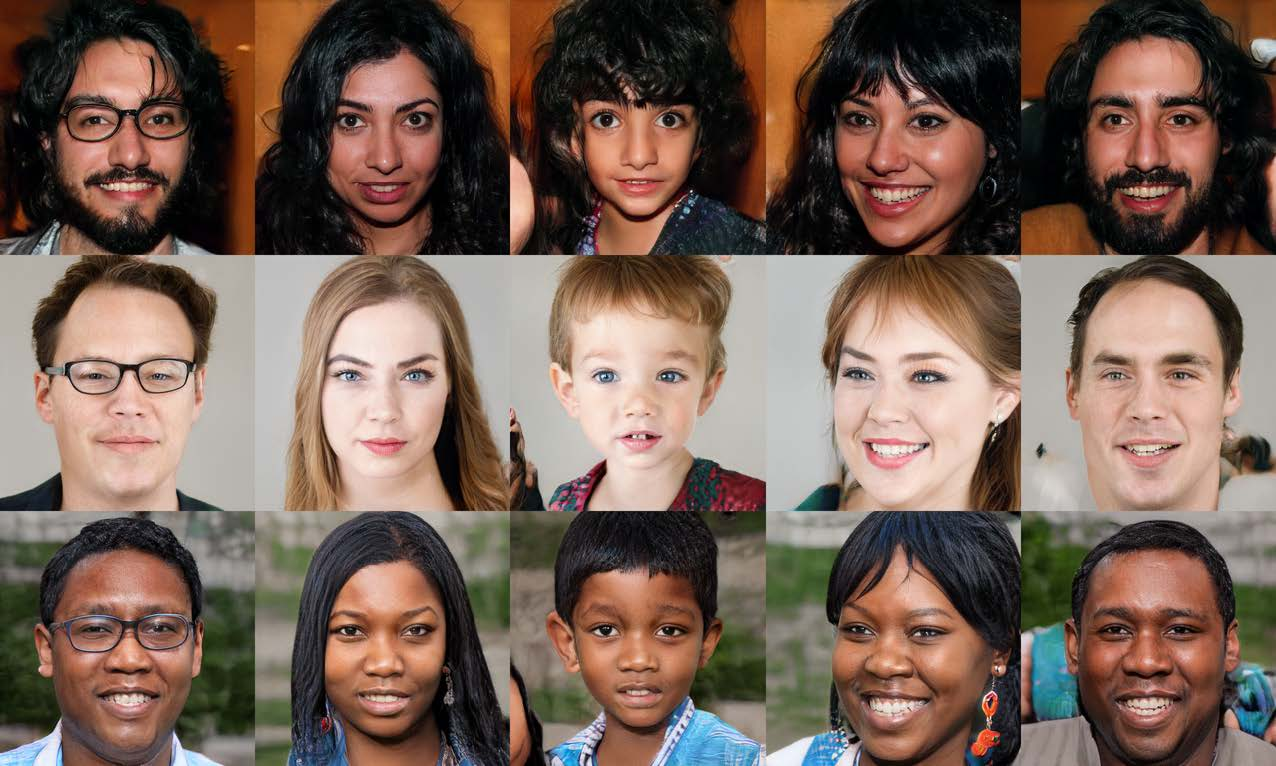
\includegraphics[width=8cm]{fig_8_1.jpg} 
	\caption{Faces generated by StyleGAN (NVIDIA), March 2020}\label{fig_8_1}
\end{figure}
\par Generally speaking, machine learning for synthesis (or generation) is more fascination than analysis (or recognition). If we have a generative model, rather than a discriminate model providing prediction for labels, we have much more details for what a computer has learned, and we are able to check where are the perceptible mistakes and improve our models. Recent developments in this area open up vastly new possibility for machine learning bringing breakthroughs in fields like animation, games, movies, art and mixed reality. Probably we are witnessing a revolution about how artificial worlds will be created, and how artificial things will be embedded into our real worlds. Though we are really only at the beginning, we will discuss several methods that we deal with in this fascinating area.
\section{Variational Autoencoders}
As the name suggests, VAEs is basically using the idea of Autoencoders (Chapter 1) that performs dimension reduction, take the data, compress it to some lower dimensional space, and then be able to reconstruct from that low dimensional thing. The key idea of VAEs, also GANs, is that if we want to sample or generate random things, we need to put some randomness into our mechanisms. 
\subsection{Deep Generative Models}
\par Since DNNs have the power to create complex distributions, we can start by sampling random vectors from a simple distribution, say a $m$-dimensional Gaussian: $\mathbb{R}^{m}\ni {\bf z}\sim \mathcal{N}(0,{\bf I})$ (it can be other distributions as well, it doesn't really matter). We then take this random vector, plug it into a network to output a sample, say an image. The idea is based on that DNNs can implement really complex transformations (recall that in image classification the learned mapping is from thousands of pixels to a single label). Here we go the other way: given a random vector, we use a deep network to transform it into something like a face, and if we sample the random vectors we sample in the face space. 
\par Formally, we want to transform random vectors though a (deterministic) deep network $F_{\theta}:\mathbb{R}^m\rightarrow\mathbb{R}^n$ parametrized by some $\theta$ with usually $n\gg m$. For example, with $n$, as the number of pixels in a image, say $40000$, $m$ might be only few hundreds. The distribution of ${\bf z}$ together with $F_{\theta}$ induce a (possibly complex) distribution over $\mathbb{R}^n$ with parameters $\theta$. This distribution is easy to sample: we can sample ${\bf x}$ by sampling ${\bf z}$ and setting ${\bf x}=F_{\theta}({\bf z})$. By the \emph{law of the unconscious statistician} we can compute the expectations over the induced distribution of any function $f({\bf x})$:
\begin{equation}\label{eq_8_lotus}
	\mathbb{E}_{\bf x}[f({\bf x})]=\mathbb{E}_{\bf z}[f(F_{\theta}({\bf z}))].
\end{equation}
This proposition is known as the law of the unconscious statistician because students have been accused of using the identity without realizing that it must be treated as the result of a rigorously proved theorem, not merely a definition (comment from Wiki). A short proof for a invertable and differentiable $F_{\theta}({\bf z})$ with continuous random variables goes as follow (while the law holds for more general functions)
\begin{align*}
	\mathbb{E}_{\bf x}[f({\bf x})]&=\int p_{\bf x}({\bf x})f({\bf x})d{\bf x}\\
		&=\int \left|\frac{\partial F_{\theta}^{-1}({\bf x})}{\partial {\bf x}} \right|f({\bf x})p_{\bf z} (F_{\theta}^{-1}({\bf x})) d{\bf x}\ \text{(change of variables formula)}\\
		&=\int p_{\bf z}({\bf z})f(F_{\theta}({\bf z}))d{\bf z}\ ({\bf z}=F_{\theta}^{-1}({\bf x}),\ d{\bf z}=\left|\frac{\partial F_{\theta}^{-1}({\bf x})}{\partial {\bf x}} \right|d{\bf x})\\
		&=\mathbb{E}_{\bf z}[f(F_{\theta}({\bf z}))].
\end{align*}
According to (\ref{eq_8_lotus}), if we want to compute the expectation w.r.t. to the induced distribution over the high-dim space, we could get that expectation by sampling ${\bf z}$ from that simpler distribution, sending ${\bf z}$ through the mapping $F_{\theta}$, and averaging them. Why is this relevant? Because it says that to compute the expectations we don't need to know the density of ${\bf x}$ if we know the density of ${\bf z}$. Since in the discussions involving distributions, very often we need to compute expectations (usually via sample approximation) which can be obtained in this way, no matter what $f({\bf x})$ is.
\begin{remark}
	We know with the DNN, a distribution on a low-dimensional space induces a distribution over a higher-dimensional space. However, it's clear that it will not fill that space if $F_{\theta}$ is differentiable from ReLU and things we use. In general the network finds a manifold in that high-dim space, which actually makes sense since as mentioned, in many cases the data are believed to be highly structured in a sense that they lie in a manifold or are sparse in some basis (e.g. it is believed that natural images are sparse in wavelet basis as we will see in the following chapters). 
\end{remark}
\par Usually the way we think about statistical model for generating data is in terms of densities. Recall that we have a simple distribution over ${\bf z}$ with the corresponding generated data ${\bf x}$ (say a face) induced by a deterministic function $F_{\theta}$ implemented by a DNN: ${\bf x}=F_{\theta}({\bf z})$. Then if $F_{\theta}$ is invertable as well, we can compute the density of ${\bf x}$ in terms of the one of ${\bf z}$ by the \emph{change of variable formula}:
\begin{equation}\label{eq_8_chg_var}
	{\bf x}=F_{\theta}({\bf z}),\quad \underbrace{p_{\bf x}({\bf x})}_{{\bf x}-\text{density}}=\left|\frac{\partial F_{\theta}^{-1}({\bf x})}{\partial {\bf x}}\right|\underbrace{p_{\bf z}(F_{\theta}^{-1}({\bf x}))}_{{\bf z}-{\rm density}}.
\end{equation}
Specifically, we would find the pre-image ${\bf z}$ that is mapped to ${\bf x}$ by $F_{\theta}$. Then we could compute the density of that pre-image ${\bf z}$, and then we adjust for the volume effect: how much distortion of the volume is locally happening, which is captured by the inverse Jacobian determinant. The density of ${\bf x}$ is useful since with it we can do things like maximum likelihood estimation given some real data by computing their likelihood function via (\ref{eq_8_chg_var}). However, in practice this will be problematic since it requires to 
\begin{itemize}
	\item find the network inversion
	\item compute the inverse Jacobian determinant
	\item compute gradients with respect to $\theta$ to learn,
\end{itemize}
some of which are often impossible (non-invertible) or intractable/impractical (dimensionality) avoiding the attempt to construct density directly. For simple $F$ this is okay, but for models we are interested in, i.e. deep models, this shows not much practical success.
\subsection{Evidence Lower Bound}
What can we do if the attempt to get density and evaluate the likelihood function doesn't work? One thing that does work is to apply the principle we have seen in the EM algorithm. In the context here, it refers to the variational lower bound or Evidence Lower BOund (ELBO). 
\par Specifically, instead of using a deterministic $F_{\theta}$, we relate ${\bf x}$ to ${\bf z}$ via a slightly more general way, a conditional distribution $p_{\theta}({\bf x}|{\bf z})$ parametrized by some $\theta$. This setting allows a little bit noise. Then together with the distribution of the latent variable $p({\bf z})$, we can define a complete data model that is given by
\begin{equation*}
	p_{\theta}({\bf x},{\bf z})=p_{\theta}({\bf x}|{\bf z})p({\bf z}).
\end{equation*}
Integrating out ${\bf z}$ yields
\begin{equation*}
	p_{\theta}({\bf x})=\int p_{\theta}({\bf x},{\bf z})d{\bf z} = \int p_{\theta}({\bf x}|{\bf z})p({\bf z})d{\bf z},
\end{equation*}
which is the marginal likelihood of ${\bf x}$. At this point, one might attempt to maximize the marginal likelihood directly, but we may not know how to perform the integration. Recall what we have seen in EM, to maximize the log marginal likelihood, we can maximize a lower bound of it instead. Again, we first introduce a variational distribution $q_{\phi}({\bf z};{\bf x})$ and rewrite the log-likelihood as
\begin{equation*}
	\log p_{\theta}({\bf x})=\log \int q_{\phi}({\bf z};{\bf x}) \frac{p_{\theta}({\bf x}|{\bf z})p({\bf z})}{q_{\phi}({\bf z};{\bf x})}d{\bf z} = \log \mathbb{E}_{q_{\phi}} \left[\frac{p_{\theta}({\bf x}|{\bf z})p({\bf z})}{q_{\phi}({\bf z};{\bf x})}\right].
\end{equation*}
\begin{remark}
	In the CIL slides, the notation ($q_\phi({\bf z}|{\bf x})$ or $q_\phi({\bf z};{\bf x})$) is inconsistent. To avoid unnecessary confusions, we use the latter one for the whole chapter. One can interpret it as the conditional distribution given ${\bf x}$ (as our VAE model is trying to model this), but as a variational distribution, it only has to be a distribution over ${\bf z}$ (that's why in PRML it just wrote $q_\phi({\bf z})$ instead). The notation of $q_\phi({\bf z};{\bf x})$ is just to emphasize it is a distribution over ${\bf z}$ with possible dependencies on ${\bf x}$.
\end{remark}
Use the concavity and apply the Jensen's inequality yields
\begin{align*}
	\log p_{\theta}({\bf x})\geq {\rm ELBO}(\phi, \theta)&=\mathbb{E}_{q_{\phi}}\left[\log p_{\theta}({\bf x}|{\bf z}) + \log \frac{p({\bf z})}{q_{\phi}({\bf z};{\bf x})} \right]\\
	&=\mathbb{E}_{q_{\phi}}\left[\log p_{\theta}({\bf x}|{\bf z})\right] - {\rm KL}(q_{\phi}({\bf z};{\bf x})||p({\bf z})),
\end{align*}
where ${\rm KL}(q||p)$ is the Kullback-Leibler divergence, which is a measure of distance between distributions. Just as in EM, we can alternatively
\begin{itemize}
	\item maximize w.r.t. $\theta$ (generative model, given $q_{\phi}$), M step in EM;
	\item maximize w.r.t. $\phi$ (inference model, given $p_\theta$), E step in EM. 
\end{itemize}
For a discussion for general EM and what do E and M step do please refer to section \ref{sec_4_EM_in_gen}. Usually in E step maximizing  w.r.t. $\phi$ means we need to compute the posterior of latent variable $p_{\theta^{\rm old}}({\bf z}|{\bf x})$ w.r.t. the old parameters, but for deep models it's too complicated. Instead, we try to compute some approximation via updates with specifically designed $q_{\phi}$.
\par Before the discussion of how we can maximize w.r.t. $\theta$ and $\phi$, let us see the VAE in a big picture that is a bit more abstract. A typical VAE can be represented in a diagram shown in Figure \ref{fig_8_2}. The right half is the generative path, where we sample ${\bf z}$ and pass it through a network to generate data ${\bf x}$ (note that this is done by sampling from the distribution $p_\theta({\bf x}|{\bf z})$ determined by the generative model). The left half is the inference path, where we do the opposite: conditioning on a data point ${\bf x}$, we want to find good Gaussian vectors ${\bf z}$ for that data ${\bf x}$, which is done in a probabilistic way (output a distribution $q_{\phi}({\bf z};{\bf x})$ rather than a deterministic value). The inference model encodes ${\bf x}$ (probabilistically) as a vector ${\bf z}$ in a much more lower dimensional space, while the generative model decodes ${\bf z}$ to produce data point ${\bf x}$. During the train, since we do thing in an unsupervised manner, we want the loop to produce or approximate in some sense the identity mapping.
\begin{figure}[h] 
	\centering 
	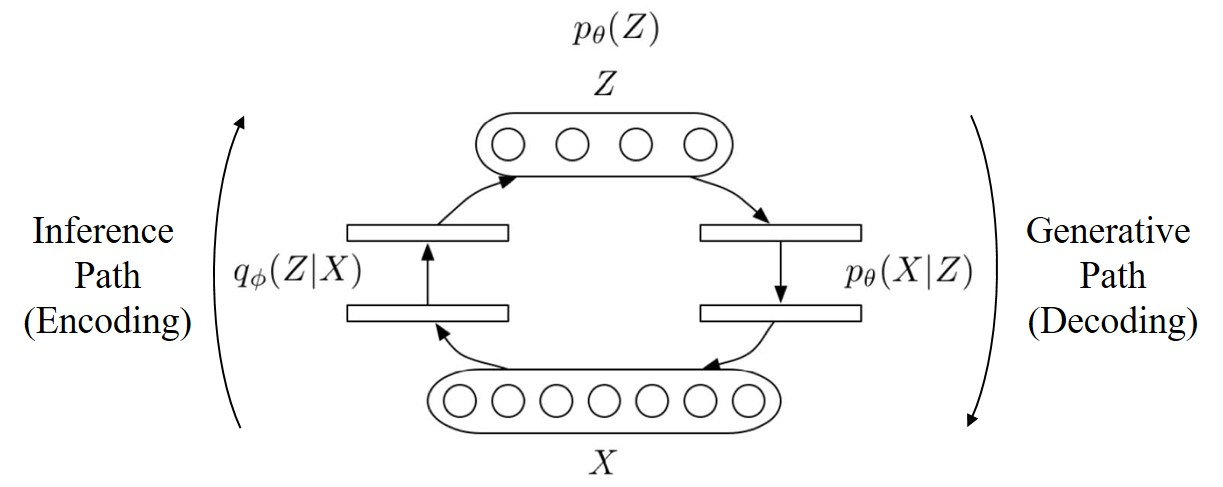
\includegraphics[width=12cm]{fig_8_2.jpg} 
	\caption{The diagram of VAE.}\label{fig_8_2}
\end{figure}
\subsection{ELBO: Generative Model Updates}
To maximize the ELBO w.r.t. $\theta$ (update the generative model), we need to be able to compute the gradients w.r.t. $\theta$. The idea is to apply a technique called \emph{stochastic approximation}. Specifically, with the observation that only the first term in ELBO depends on $\theta$ we can do the following
\begin{equation*}
	\nabla_{\theta}\mathbb{E}_{q_{\phi}}[\log p_\theta({\bf x}|{\bf z})] = \mathbb{E}_{q_{\phi}}[\nabla_{\theta}\log p_\theta({\bf x}|{\bf z})].
\end{equation*}
Here we apply the Leibniz integral rule which allows us to exchange $\mathbb{E}_{q_\phi}$ and $\nabla_{\theta}$. This rule does not always hold but for all the cases we are interested in. For the expectation, if we have $q_\phi$ we can compute a simple Monte Carlo approximation of it by sampling from $q_\phi$. Therefore, we obtain
\begin{equation*}
	\nabla_{\theta}\mathbb{E}_{q_{\phi}}[\log p_\theta({\bf x}|{\bf z})] \approx \frac{1}{L}\sum_{r=1}^{L} \nabla_{\theta}\log p_\theta({\bf x}|{\bf z}^{(r)}),\ {\bf z}^{(r)}\overset{i.i.d}{\sim}q_\phi(\cdot;{\bf x}),
\end{equation*}
where $L$ is the number of sample and is a hyperparameter. For a fixed ${\bf z}^{(r)}$, $\nabla_{\theta}\log p_\theta({\bf x}|{\bf z}^{(r)})$ is the network gradient which can be obtained with backpropagation. (As shown in Figure \ref{fig_8_2}, the generative model outputs a conditional probability distribution over ${\bf x}$ given ${\bf z}$ rather than a deterministic value. This is a little bit different from the networks we have seen.) This Monte Carlo approximation produces an unbiased gradient estimate (SGD). The gradient is obtained in a sense that is similar to supervised learning, where we have ${\bf z}$ as the input and use the output ${\bf x}$ to compute the gradient. To show how this is done, for a Gaussian observation model
\begin{equation}\label{eq_8_gau_obs}
	p_\theta({\bf x}|{\bf z})=\mathcal{N}(F_\theta({\bf z}), {\bf I}),
\end{equation}
the gradient is generated via a squared error $\frac{1}{2}\|F_\theta({\bf z})-{\bf x}\|^2$.
\par The updates for the generative model turns out to be the easy part in the maximization of ELBO. The inference model performs approximate model inversion in a way that given ${\bf x}$ it finds a reasonable ${\bf z}$. Determine the gradient w.r.t. $\phi$ turns out to be more tricky, and we will discuss it in the next section.
\subsection{ELBO: Inference Model Updates}
Let us first look at the update step for the inference model in an abstract view. For a general function $\mathcal{L}({\bf x,z})$, given ${\bf x}$ and ${\bf z}\sim q_\phi({\bf z};{\bf x})$, the gradient w.r.t. $\phi$ of the expectation of $\mathcal{L}({\bf x,z})$ (w.r.t. $q_\phi$) is given by
\begin{equation*}
	\nabla_\phi \mathbb{E}_{q_\phi}[\mathcal{L}({\bf x,z})] = \underbrace{\int \mathcal{L}({\bf x,z}) \nabla_\phi q_\phi({\bf z};{\bf x})d{\bf z}}_{\text{still intractable}}=\mathbb{E}[?]
\end{equation*}
where again we have applied the Leibniz rule. Different from the generative model, here the dependency on $\phi$ is in the expectation. We can apply the Leibniz rule, but the result is not obviously in an expectation form. Note that if so we can again apply the Monte Carlo approximation by sampling and averaging. Following this idea, one way to rewrite the gradient into a form of expectation is by applying the \emph{reinforce trick} (Williams 1992):
\begin{equation*}
		\nabla_\phi \mathbb{E}_{q_\phi}[\mathcal{L}({\bf x,z})] =  \mathbb{E}_{q_\phi}[\mathcal{L}({\bf x,z})	\nabla_\phi\log q_\phi({\bf z};{\bf x})],
\end{equation*}
where we have used
\begin{equation*}
	\nabla q = q\nabla\log q.
\end{equation*}
Then we can estimate the gradient via sampling, but despite the unbiasedness of this estimation, the variance is usually very high, which requires impractically large number of samples to guarantee a accurate estimation. Nevertheless, this reinforce trick can already be a feasible way to update the inference model. By doing so we have completed the map of optimizing VAEs.
\par Another way to make the gradient some expectations is by applying the \emph{re-parameterization trick}. Instead of allowing any variational distribution $q_\phi$, we use $q_\phi$ such that
\begin{equation*}
	{\bf z} = g_\phi(\zeta;{\bf x})\quad \text{and}\quad{\bf z}\sim q_\phi({\bf z};{\bf x}).
\end{equation*}
where
\begin{equation*}
	\zeta\sim \text{ simple distribution (e.g. }\mathcal{N}({\bf 0,I})).
\end{equation*}
What we are doing here is basically a change of variable. We transform a very simple random variable $\zeta$ using a function $g_\phi(\cdot;{\bf x})$ (${\bf x}$ is its parameter) such that the resulting random variable ${\bf z}=g_\phi(\zeta;{\bf x})$ obeys $q_\phi({\bf z};{\bf x})$, i.e. ${\bf z}\sim q_\phi({\bf z};{\bf x})$. With this re-parameterization, the gradient of expectation can be converted into expectation of gradient (known as \emph{stochastic backpropagation}). Specifically, first recall the law of the unconscious statistician (LOTUS) (\ref{eq_8_lotus}), we can rewrite the gradient of expectation as
\begin{align*}
	\nabla_\phi \mathbb{E}_{{\bf z}\sim q_\phi}[\mathcal{L}({\bf x,z})] &= \nabla_\phi \mathbb{E}_{\zeta\sim\mathcal{N}({\bf 0,I})} [\mathcal{L}({\bf x},g_\phi(\zeta;{\bf x}))]\ ({\rm LOTUS})\\
	&=\mathbb{E}_{\zeta}[\nabla_\phi \mathcal{L}({\bf x},g_\phi(\zeta;{\bf x}))]\ (\text{Leibniz rule})\\
	&\approx \frac{1}{L}\sum_{r=1}^{L}[\nabla_\phi \mathcal{L}({\bf x},g_\phi(\zeta^{(r)};{\bf x}))],\ \zeta^{(r)}\overset{i.i.d.}{\sim}\mathcal{N}({\bf 0,I}),
\end{align*}
where $\zeta$ can obey other simple distributions as well. As an example, consider $\zeta\sim\mathcal{N}({\bf 0,I})$. If we define
\begin{equation*}
	{\bf z} = g_\phi(\zeta;\underbrace{\mu,{\bf U}}_{\phi})=\mu +{\bf U}\zeta.
\end{equation*}
Then
\begin{equation*}
	{\bf z}\sim \mathcal{N}(\mu,{\bf UU}^T).
\end{equation*}
In practice, it is often observed that re-parameterization trick leads to lower variance estimates than the reinforce trick, but this does not mean that the re-parameterization is in a sense consistently better than the other one (no theoretical results).
\subsection{Deep Latent Gaussian Models}
Now we look at an instantiation of the VAE framework we have just discussed about, namely the Deep Latent Gaussian Models (DLGM). In DLGM, we inject randomness in a simple form at each layer to the deep model.  Specifically, for each layer we define a noise variable
\begin{equation*}
	{\bf z}^l\overset{i.i.d.}{\sim}\mathcal{N}({\bf 0,I}),\ l=1,\dots,L.
\end{equation*}
Let ${\bf x}^l$ be the activation for layer $l$. We start from the generative model of DLGM with top-down-indexed layers (we start from the $L$-th layer all the way to ${\bf x}^1$ from which we can sample data points). The forward propagate starts from the $L$-th layer with
\begin{equation*}
	{\bf x}^L={\bf W}^L{\bf z}^L.
\end{equation*}
The intermediate hidden activities (latent random variables) act in the following way:
\begin{equation*}
	{\bf x}^l=\underbrace{F^l({\bf x}^{l+1})}_{\rm deterministic}+\underbrace{{\bf W}^l{\bf z}^l}_{\rm stochastic},
\end{equation*}
where the first term is deterministic with the layer mapping $F^l$, and the index $l+1$ shows that we are propagating top-down; the second term shows that we always inject randomness in each layer (via a linear transform of a part of latent variable ${\bf z}=({\bf z}^1,\dots,{\bf z}^L)$, see also remark \ref{rmk_8_1}). The hidden layer (conditional) distribution is then
\begin{equation*}
	{\bf x}^l|{\bf x}^{l+1}\sim \mathcal{N}\left(F^l({\bf x}^{l+1}),{{\bf W}^l{\bf W}^l}^T\right).
\end{equation*}
Finally, we generate pattern ${\bf x}\sim \pi({\bf x}^l)$, where $\pi(\cdot)$ is an observation/noise model with parameter ${\bf x}^1$ (as an example: the Gaussian observation model (\ref{eq_8_gau_obs})).

\par For the inference model of DLGM, first recall that given ${\bf x}$ the inference model helps to find ${\bf z}$ that we have to inject to the generative model to produce such a ${\bf x}$. In DLGM, ${\bf z}$ consist of all randomness injected in each layer (known as amortized inference):
\begin{equation*}
	{\bf z} =({\bf z}^1,\dots,{\bf z}^L).
\end{equation*}
Assume we draw ${\bf z}^l$ independently. The variational distribution $q_\phi({\bf z};{\bf x})$ is given by
\begin{equation*}
	q_\phi({\bf z};{\bf x})=\prod_{l=1}^{L}\mathcal{N}({\bf z}^l|\mu^l({\bf x}),{\bf C}^l({\bf x})),\quad {\bf C}^l({\bf x})={\bf U}^l({\bf x}){\bf U}^l({\bf x})^T,
\end{equation*}
where $\mu$ and $\bf U$ are represented by DNNs with input $\bf x$. The update equations for $\mu$ in the inference model can be obtained using the Bonnet formula (for ${\bf z}\sim \mathcal{N}(\mu,{\bf C})$):
\begin{equation*}
	\nabla_\mu\mathbb{E}_{\bf z}[f({\bf z})]=\mathbb{E}_{\bf z}[\nabla_{\bf z} f({\bf z})].
\end{equation*}
Here's a brief proof for the Bonnet formula:
\begin{align*}
	\nabla_{\mu_i}\mathbb{E}_{\mathcal{N}(\mu,{\bf C})}[f({\bf z})] &= \int  \nabla_{\mu_i} \mathcal{N}({\bf z}|\mu,{\bf C}) f({\bf z}) d{\bf z}\\
	&=-\int \left[\nabla_{z_i}\mathcal{N}({\bf z}|\mu,{\bf C})\right] f({\bf z}) d{\bf z}\\
	&=\left[\int\mathcal{N}({\bf z}|\mu,{\bf C}) f({\bf z}) d{\bf z}_{\neg i} \right]_{z_i=-\infty}^{z_i=\infty}+ \int \mathcal{N}({\bf z}|\mu,{\bf C}) \nabla_{z_i} f({\bf z}) d{\bf z}\\
	&=\mathbb{E}_{\mathcal{N}(\mu,{\bf C})}[\nabla_{z_i}f({\bf z})].
\end{align*}
For ${\bf U}$, we can use the re-parameterization trick. Recall that we have ${\bf z}\sim \mathcal{N}(\mu,{\bf C})$, and this can be re-parameterized by ${\bf z}={\bf U}\zeta +\mu,\ \zeta\sim\mathcal{N}(0,{\bf I})$. Then LOTUS yields
\begin{equation*}
	\nabla_{\bf U}\mathbb{E}_{\bf z}[f({\bf z})]=\nabla_{\bf U}\mathbb{E}_\zeta[f({\bf U}\zeta +\mu)]=\mathbb{E}_\zeta[\zeta^T{\bf g}],\ {\bf g}:=\nabla_\xi f(\xi)_{|\xi={\bf U}\zeta+\mu},
\end{equation*}
where we have used the chain rule for composition of a function with a linear function.
\begin{remark}\label{rmk_8_1}
	In Figure \ref{fig_8_2}, the diagram seems to require the model (networks) to give $q_\phi({\bf z};{\bf x})$  at the last layer of the inference model. However, as the deep latent Gaussian models suggest, this is not the case in the sense that the model can generate the distribution of a part of ${\bf z}$ at the intermediate layers. So we see that the VAE shown in Figure \ref{fig_8_2} is an abstract framework, and $q_\phi({\bf z};{\bf x})$ and $p_\theta({\bf x}|{\bf z})$ don't even have to be produced by a deep model, but other models work as well.
\end{remark}
\begin{remark}
In the original paper (Rezende et al. 2014), the Price's Theorem and Gaussian backpropagation refer to different things, so there might be some name misusing.
\end{remark}
Finally we can have a look at the big picture of DLGM. As illustrated in Figure \ref{fig_8_3}, DLGM consists of 2 parts: the generative model on the left and the recognition (inference) model on the right. The red arrows in the image represent propagation in learning, while the black ones are the forward passes. 
\par To generate new data point ${\bf x}$, we sample ${\bf z}^l\sim \mathcal{N}(\mu^l,{\bf C}^l)$ with given $(\mu^l,{\bf C}^l)$ (black horizontal dotted arrows); the activation ${\bf x}^l$ are sampled from $ \mathcal{N}\left(F^l({\bf x}^{l+1}),{{\bf W}^l{\bf W}^l}^T\right)$ (black vertical dotted arrows). The red arrows in generative model shows how the backpropagation goes along the layers. Given ${\bf x}_0$ and ${\bf z}$ produced by the inference model $q_\phi({\bf z}|{\bf x}_0)$, the gradients are obtained by the error $l(x_0,{\rm Gen}({\bf z}))$, where ${\rm Gen}({\bf z})$ is an output of the generative model with ${\bf z}$.
\par The inference model is similar. The forward pass represented by black arrows are deterministic given ${\bf x}$, since $\{\mu({\bf x}), {\bf C}({\bf x})\}$ are deterministic functions w.r.t. ${\bf x}$. The red dashed arrows are stochastic backpropagation, where we use the re-parameterization trick and need to sample $\zeta\sim \mathcal(0,{\bf I})$.
\begin{figure}[h] 
	\centering 
	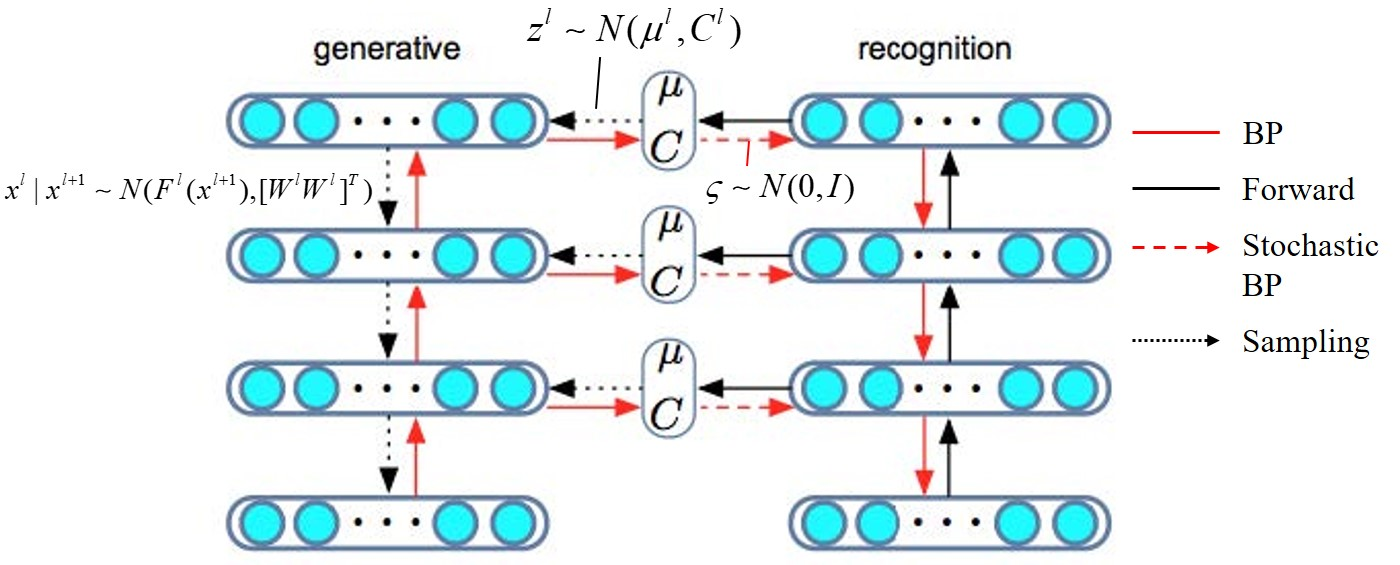
\includegraphics[width=12cm]{fig_8_3.jpg} 
	\caption{Learning and forward propagation scheme for Deep Latent Gaussian Models.}\label{fig_8_3}
\end{figure}
\par Here is some example generated by VAEs. As we can see that they are not bad but kind of blurry (Figure \ref{fig_8_4}). We will another type of model that is able to generate better results in the next section.
\begin{figure}[h] 
	\centering 
	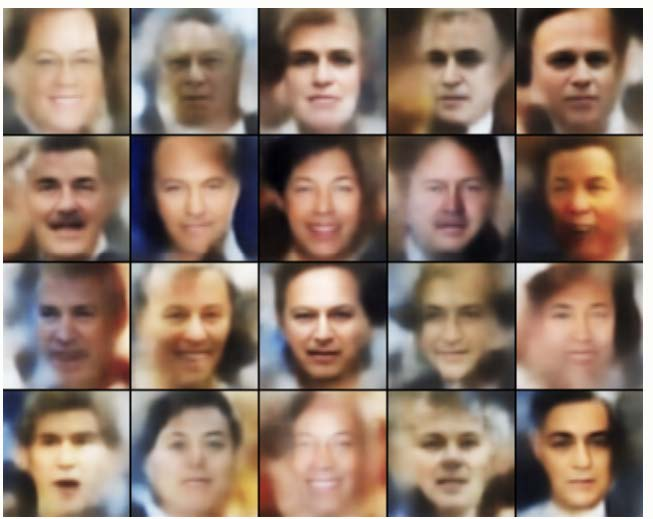
\includegraphics[width=6cm]{fig_8_4.jpg} 
	\caption{Face generation via VAEs.}\label{fig_8_4}
\end{figure}
\section{Generative Adversarial Networks}
GANs, proposed by Goodfellow et al.,2014, are something better known than VAEs. The idea is also more straightforward: given some data, say faces, generated by some devices and also some real faces, if there's a way that somehow we can discriminate these faces this could provide an error signal to the generator. In another word, we want to have a classifier/discriminator to train the generator.
\par Let us make this idea concrete by defining a formal classification problem, where we have a mixed source of data: half forms by the real ones and the other by the generated ones. Denote a data sample by ${\bf x}$ and the corresponding label by ${y}$ indicating whether it is real ($y=1$) or not ($y=0$), we can then define th joint distribution of $({\bf x},y)$ as mixture by
\begin{align*}
	&\tilde{p}_\theta({\bf x},y=1)=P(y=1)P({\bf x}|y=1)=\frac{1}{2}p({\bf x})\\
	&\tilde{p}_\theta({\bf x},y=0)=P(y=0)P({\bf x}|y=0)=\frac{1}{2}p_\theta({\bf x}),
\end{align*}
where $\tilde{p}_\theta$ denotes the distribution of mixed data with $p({\bf x})$ and $p_\theta({\bf x})$ representing the distribution of real data and generated data respectively. Before we discuss how this setting can benefit our learning, let us first think about what is the best can a discriminator do. The answer is given by the Bayes optimal classifier, i.e. making decision based on the posterior $P(y|{\bf x})$:
\begin{equation*}
	P(y=1|{\bf x}) = q_\theta=\frac{p}{p+p_\theta},\ {\rm output}\ y=\begin{cases}
	1 & {\rm if}\ q_\theta>\frac{1}{2}\\
	0 & {\rm otherwise}
	\end{cases}.
\end{equation*}
The goal of a generator is to generate samples that are indistinguishable from the real data, even for the best possible classifier, i.e. the Bayes optimal classifier. Specifically, we want to train a generator via minimizing the logistic likelihood for the discriminators, particularly for the best possible one:
\begin{equation*}
	\theta\overset{\min}{\rightarrow}l^*(\theta):=\mathbb{E}_{\tilde{p}_\theta}[y\ln q_\theta({\bf x})+(1-y)\ln(1-q_\theta({\bf x}))].
\end{equation*}
It can be shown that
\begin{equation*}
	l^*(\theta)={\rm JS}(p,p_\theta)-\ln 2,
\end{equation*}
where ${\rm JS}$ is the Jensen-Shannon divergence which measures distance between distributions. From this we can see that, to train a generator that minimize $l^*(\theta)$, we need to make $p_\theta \approx p$. In practice, we have no access to these two distributions and cannot compute the JS-divergence. The discussion here just aims at giving some theoretical intuition.
\par If we have no access to $p$ and $p_\theta$, the optimal classifier is in general inaccessible. Instead, we can define a classification model, just as in VAEs we introduce a second model, given by
\begin{equation*}
	q_\phi:{\bf x}\rightarrow [0,1],\quad \phi\in\Phi,
\end{equation*}
where $\phi$ represent model parameters and $\Phi$ is the class of functions (weight space for DNN model). By optimality, plugging in any classifier to the logistic likelihood will result in a lower bound for $l^*(\theta)$, so to get it close to the Bayes optimal we take $\sup$ over $\Phi$:
\begin{equation*}
	l^*(\theta)\geq\sup_{\phi\in\Phi}l(\theta,\phi),\quad l(\theta,\phi) :=\mathbb{E}_{\tilde{p}_\theta}[y\ln q_\phi({\bf x})+(1-y)\ln(1-q_\phi({\bf x}))].
\end{equation*}
Taking sup means finding the best classifier within the restricted family ${\Phi}$. While for the generator, it wants to make the likelihood low for all possible classifiers, which means that the training objective for the generator is defined implicitly over sup:
\begin{equation*}
	\theta^*:=\mathop{\arg\min}_{\theta\in\Theta}\{\sup_{\phi\in\Phi}l(\theta,\phi)\},
\end{equation*}
where ${\Theta}$ is the class of functions for generative model from which the generator want to find a ${\theta}$ that minimize $\sup_{\phi\in\Phi}l(\theta,\phi)$. Note that in VAEs we maximize over both $\theta$ and $\phi$, but here we have an adversarial setting, also known as a \emph{saddle-point problem}. Despite we have already defined an optimization objective, explicitly performing inner sup is impractical, and solving saddle-point problem is in general very hard. Still there have been various methods from optimization and solving ``games''. But let's put these aside. The simplest thing one can do is a simultaneous SGD and Ascent (for the sup we need to do ascent instead of descent) by updating the parameters follow
\begin{align*}
	&\theta^{t+1}=\theta^t-\eta \nabla_\theta l(\theta^t,\phi^t)\\
	&\phi^{t+1}=\phi^t+\eta \nabla_\phi l(\theta^{t+1},\phi^t).
\end{align*}
Although this may diverge and has no theoretical guarantees as SGD for convex functions. Problematic cases that this fails can be easily constructed. However, this is just a staring point, and at least we can tell that one can easily train a classifier to distinguish VAE-generated data while the GANs can do better. Despite, the GANs are very hard to train, very expensive to train (many GPUs needed), and there is no clear evaluation metric (we don't know whether the models captures all important things), with efforts and proper tricks people have made it to use GANs to generate amazing results (Figure \ref{fig_8_1}).
\section{Autoregressive Models}
The last part of this chapter is about something less fascinating but easier and able to produce quite good results. These models have been used for many speech synthesis tasks.
\par Despite the generating power of VAEs and GANs, they requires complicated learning methods and are not always successful. Autoregressive models exploits a simpler strategy: generate output variable one at a time with the help of chain rule:
\begin{equation*}
	p(x_1,\dots,x_m)=\prod_{t=1}^{m}p(x_t|x_{1:t-1}).
\end{equation*}
Take image synthesis for example, to generate image pixels, we can just give the pixels some order, and conditioning on what we already have to decide what to produce next. This is exactly the idea behind PixelCNN (A. van de Oord et al. 2016), where the network models a conditional distribution for every individual pixel given previous pixels (to the left and to the top in PixelCNN, but it is just a design choice).
\begin{figure}[h] 
	\centering 
	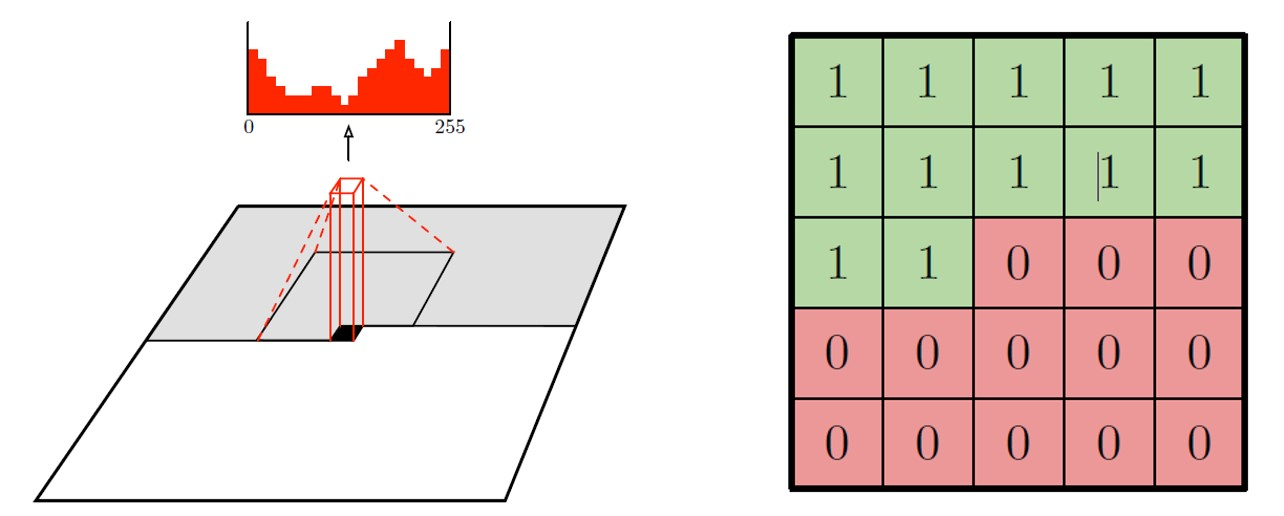
\includegraphics[width=10cm]{fig_8_5.jpg} 
	\caption{Left: PixelCNN uses previous generated pixels to help predict the next one. Right: the conditioning is equivalent to perform a masked convolution, this is why it is called CNN.}\label{fig_8_5}
\end{figure}
The way PixelCNN works is illustrated in Figure \ref{fig_8_5}. It model the joint distribution of pixels over image ${\bf x}$ as products of conditional distributions, where $x_i$ is a single pixel:
\begin{equation*}
	p({\bf x})=\prod_{i=1}^{n^2}p(x_i|x_{1:i-1}),
\end{equation*}
where $x_{1:i-1}$ are the previously generated pixels. The ordering of pixels dependencies is in a raster scan order: row by row and pixel by pixel within every row. Also, PixelCNN doesn't condition on all previous pixels, but in a sense that only for local context (the left part of Figure \ref{fig_8_5}). This can be done with a masked convolution (apply a masked filter) as shown in the right of Figure \ref{fig_8_5}.
\par The prediction of PixelCNN is sequential: every time a pixel is predicted, and it is fed back into the network to predict the next pixel. One drawback is that this might be too slow. 
\begin{figure}[h] 
	\centering 
	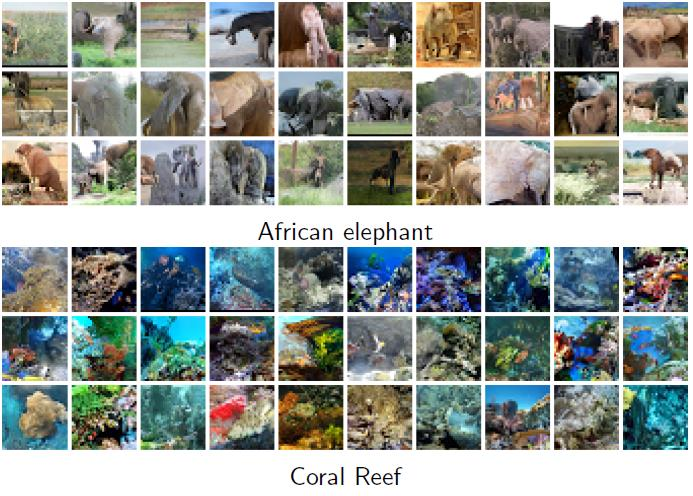
\includegraphics[width=10cm]{fig_8_6.jpg} 
	\caption{Some results from autoregressive model.}\label{fig_8_6}
\end{figure}
\par Figure \ref{fig_8_6} shows some example from PixelCNN. We see that although the quality of images are not as the ones produced by VAEs and GANs, PixelCNN still produces interesting results.


%%%%%%%%%%%%%%%%%%%%%%%%%%%%%%%%%%%%%%%%%%%%%%%%%%%%%%%
%   New Chapter                                       %
%%%%%%%%%%%%%%%%%%%%%%%%%%%%%%%%%%%%%%%%%%%%%%%%%%%%%%%

\chapter{Sparse Coding}
In this and the next chapter, we will take a classical view on representing data which is inspired from signal processing. This chapter will have less to do with machine learning but more just about ideas to represent data/signals, specifically in a sparse way, while in the next chapter we will take about how to learn these representations. Our discussion will start by requiring orthogonality for the basis with two widely used examples: Fourier basis and wavelet basis. We will then compare them with PCA in terms of data compression to put some connection back to things we have already covered. Image compression will also be briefly discussed. Then we go beyond the orthonormal basis to a new family of coding that exploits redundancy in representation to benefit sparsity. The discussion is followed by how to construct such dictionaries as well as how to reconstruct the signal based on that dictionary.
\section{Sparse Coding}
A basic observation in signal processing is that signals can be represented in different ways. For any given signal, we actually can find infinite number of possible representations, each of which usually captures different characteristics for the signal. For example, as shown in Figure \ref{fig_9_1}, a periodic signal in time domain can usually be represented in a much simpler way in terms of Fourier series. These (simple) representations, usually reveal a lot about the signals giving some useful insight and also open up other possibilities like data compression or finding better representations. 
\begin{figure}[h] 
	\centering 
	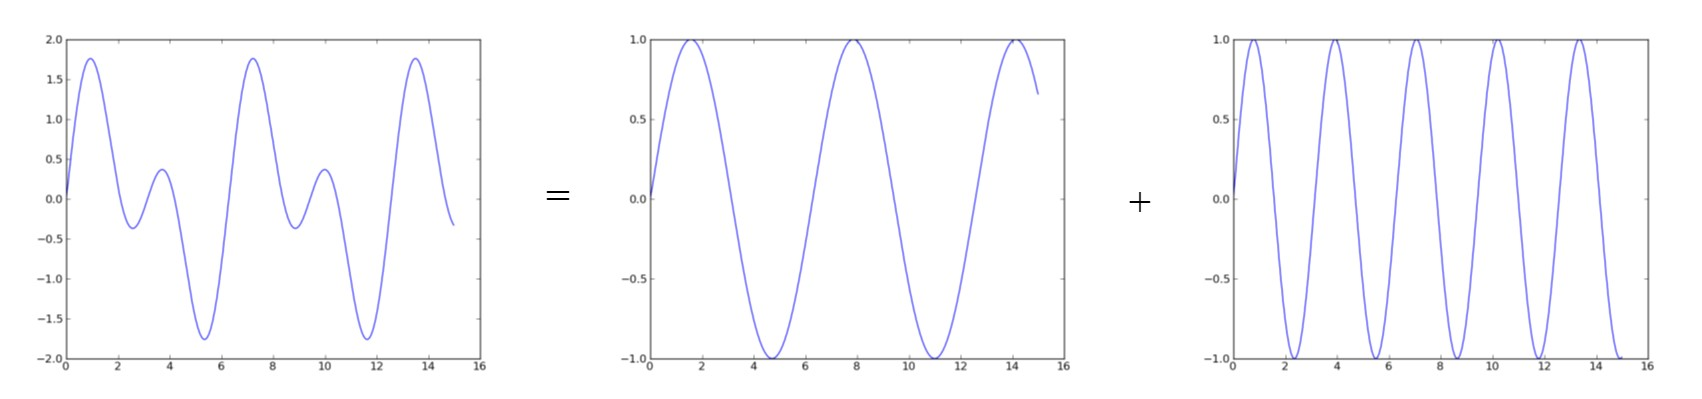
\includegraphics[width=12cm]{fig_9_1.jpg} 
	\caption{Periodic signals usually have a simple representation in Fourier basis.}\label{fig_9_1}
\end{figure}
\par Another general observation that motivates sparse coding is that natural signals often allow for sparse representation. For sparsity, we mean that in the representations many coefficients vanish ($\approx 0$) with only a few ones are non-zero. This is justified by the assumption on the regularities of signals. Just like signals for human speaking should not be any time series but forms a particularly small and highly-structured subset of all acoustic signals. To reveal the sparsity, we need to find a suitable dictionary of atoms $\mathcal{U}=\{{\bf u}_1,\dots,{\bf u}_L\}$, which can be predefined or learned from data (will be discussed in the next chapter). The original signal should have an accurate representation in span($\mathcal{U}$) with only a few atoms.
\subsection{Signal Compression}
A very simple setup we can think of as a start is the following. Given the original signal ${\bf x}\in \mathbb{R}^D$ and orthonormal matrix ${\bf U}=({\bf u}_1,\dots,{\bf u}_D)$ (the dictionary), we can re-represent ${\bf x}$ in a different basis by compute a linear transformation:
\begin{equation*}
	{\bf z}=\underbrace{{\bf U}^T}_{D\times D}\cdot {\bf x}.
\end{equation*}
As a direct consequence of orthogonality, the energy/length is preserved after the transformation in the sense that
\begin{equation*}
	\|{\bf U}^T{\bf x}\|^2 = \|{\bf x}\|^2.
\end{equation*}
Note that the preservation of length implies the preservation of angles. As a rather intuitive explanation, every angle in a triangle remains the same after orthonormal transformation (due to the fact that edges stay the same). At this point, there is no loss of information since we can reconstruct ${\bf x}$ from ${\bf z}$ by ${\bf x}={\bf Uz}$. To force sparsity, we truncate ``small'' values of ${\bf z}\Longrightarrow\hat{\bf z}$. Specifically, we encode only $K\ll D$ non-zeros values. This can be done by either only keeping the $K$ largest coefficients or employing a threshold $\epsilon$:
\begin{equation*}
	\hat{z}_d=\begin{cases}
	0 &\ {\rm if}\ |z_d|<\epsilon\\
	z_d&\ {\rm otherwise}
	\end{cases},
\end{equation*}
which is preferred since this let the data ``speak'' about how sparse should the representation be. For reconstruction, we can simple apply an inverse transform given by
\begin{equation*}
	\hat{\bf x}={\bf U}\hat{\bf z}\quad{\rm as}\ {\bf U}^T={\bf U}^{-1}.
\end{equation*}
Here we benefit from the choice of orthonormal basis for the efficient inversion. If the reconstruction error is low, then we have found a sparse representation for ${\bf x}$. To evaluate the reconstruction error, first recall that given ${\bf x}$ and orthonormal basis $\{{\bf u}_1,\dots,{\bf u}_D\}$ (columns of ${\bf U}$), ${\bf x}$ can be decomposed in the form of
\begin{equation*}
	{\bf x}=\sum_{d=1}^{D}z_d({\bf x})\cdot {\bf u}_d,\quad z_d({\bf x}):=\langle {\bf x,u}_d\rangle.
\end{equation*}
For sparsification, we keep only a $K$-subset $\sigma$ of basis functions:
\begin{equation*}
	\hat{\bf x}=\sum_{d\in \sigma}z_d({\bf x})\cdot {\bf u}_d.
\end{equation*}
This gives the reconstruction error
\begin{equation*}
	\|{\bf x}-\hat{\bf x}\|^2=\left\|\sum_{d\notin \sigma}\langle {\bf x,u}_d\rangle \cdot {\bf u}_d \right\|^2 = \sum_{d\notin \sigma}\|\langle {\bf x,u}_d\rangle \cdot {\bf u}_d\|^2 = \sum_{d\notin \sigma}\langle {\bf x,u}_d\rangle^2.
\end{equation*}
This shows that how much energy is lost in thresholding/selecting can be easily computed. Keep in mind that we are not trying to find a sparse representation for a single signal but for a class of signals, say all natural acoustic signals. We want a dictionary works for a whole range of signals, in which these signals are sparsely representable. 
\subsection{Sparse Coding with Fourier Basis and Wavelet Basis}
Now we introduce 2 examples of such orthonormal basis for 1-D signal processing, namely the Discrete Fourier Transform (DFT) and the Discrete Wavelet Transform (DWT). Take the signal shown in Figure \ref{fig_9_2} for an example.
\begin{figure}[h] 
	\centering 
	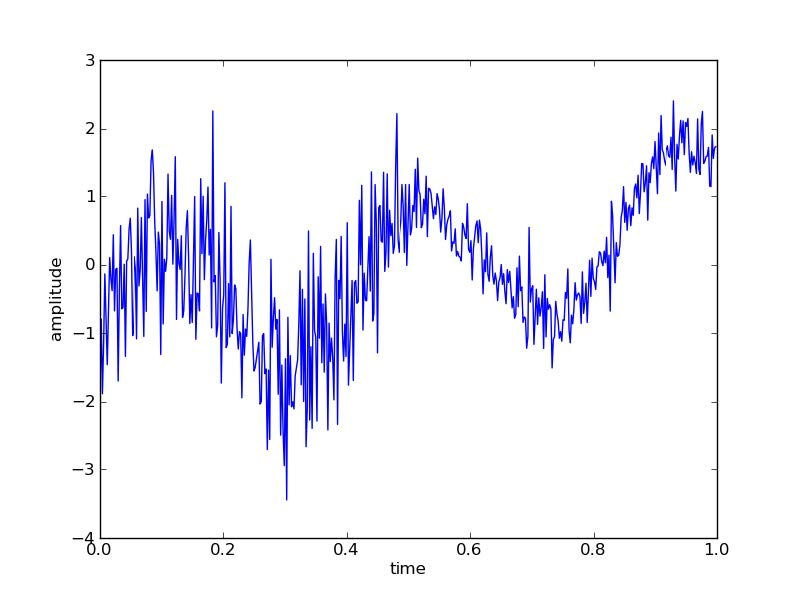
\includegraphics[width=8cm]{fig_9_2.jpg} 
	\caption{A sample signal.}\label{fig_9_2}
\end{figure}
\par We can see a trend with some high frequency noise. If we perform DFT (${\bf z}={\bf U}^T{\bf x}$) who has orthonormal basis in the form of sine functions with different frequencies and plot its spectrum (left of Figure \ref{fig_9_3}) we see that the energy concentrates in the low-frequency part. If we perform an $\epsilon$-thresholding (right of Figure \ref{fig_9_3}) and reconstruct the signal, we get a smooth signal without noise (Figure \ref{fig_9_4}), which can be regarded as being applied with a low-pass filter. Although at the boundaries, the reconstructed signal has some weird behaviors (because DFT assumes periodic signals), in the middle it covers the trend. Since we only keep $3\%$ of the Fourier coefficients, the signal is compressed by $97\%$. The high signal frequencies have small amplitudes in spectrum and therefore are suppressed. In this case, the things we have thrown away could probably be considered as noise, but there might be some useful information in some cases.
\begin{figure}[h] 
	\centering 
	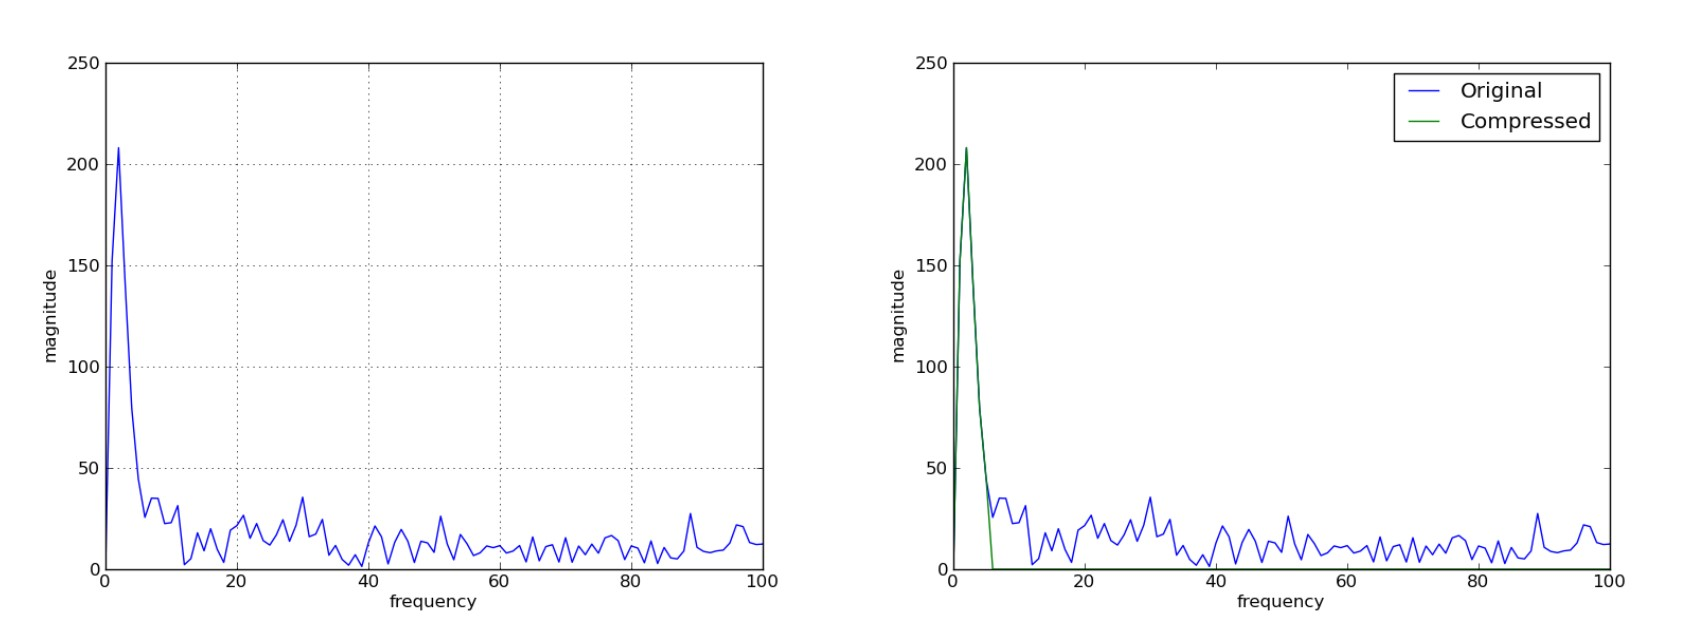
\includegraphics[width=12cm]{fig_9_3.jpg} 
	\caption{Left: Fourier spectrum of signal in Figure \ref{fig_9_2}. Right: retaining $3\%$ of the coefficients $\hat{\bf z}$.}\label{fig_9_3}
\end{figure}
\begin{figure}[h] 
	\centering 
	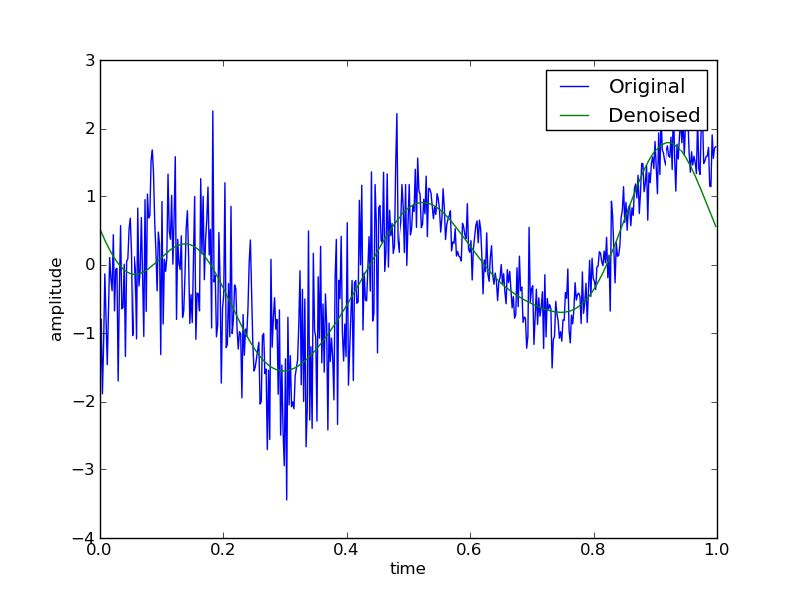
\includegraphics[width=9cm]{fig_9_4.jpg} 
	\caption{Reconstructed signal with DFT: $\hat{\bf x}={\bf U}\hat{\bf z}$ (Denoised).}\label{fig_9_4}
\end{figure}
\par However, is Fourier basis the final answer for all potentially sparse signals? Consider the another example shown in the left part of Figure \ref{fig_9_5}, which shows stronger localized properties than the last one. The denoised signal with DFT is shown in the right part, where it is clear that DFT fails completely.
\begin{figure}[h] 
	\centering 
	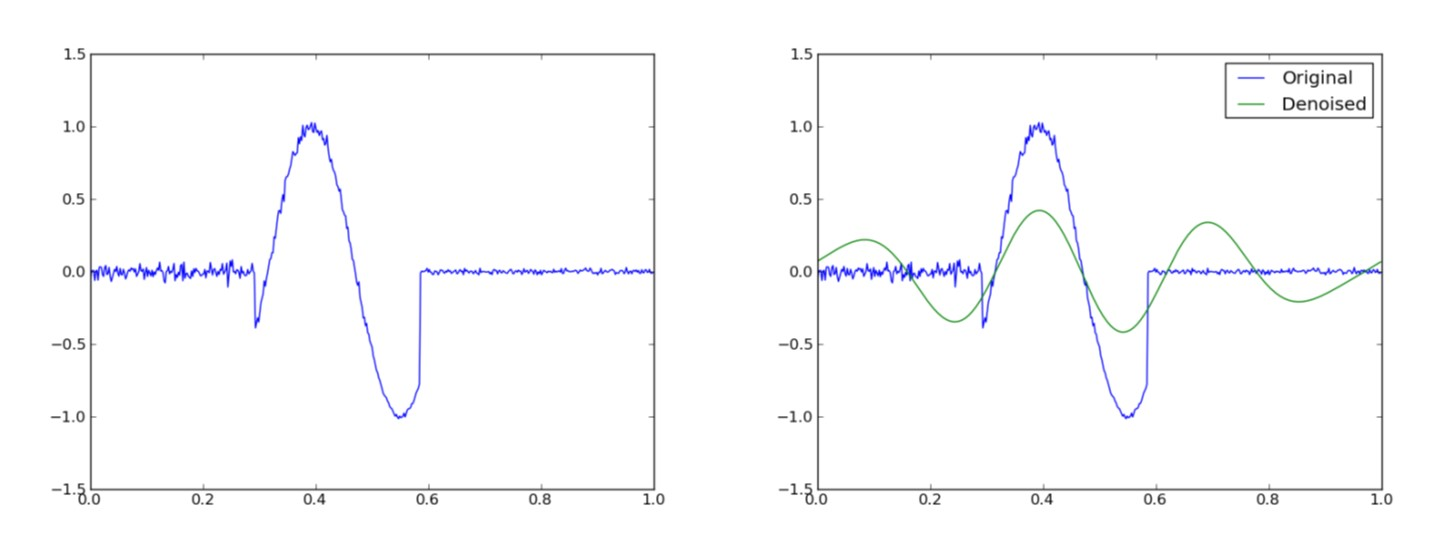
\includegraphics[width=12cm]{fig_9_5.jpg} 
	\caption{Left: a signal fail to be described with DFT. Right: the reconstruction of DFT.}\label{fig_9_5}
\end{figure}
\begin{figure}[h] 
	\centering 
	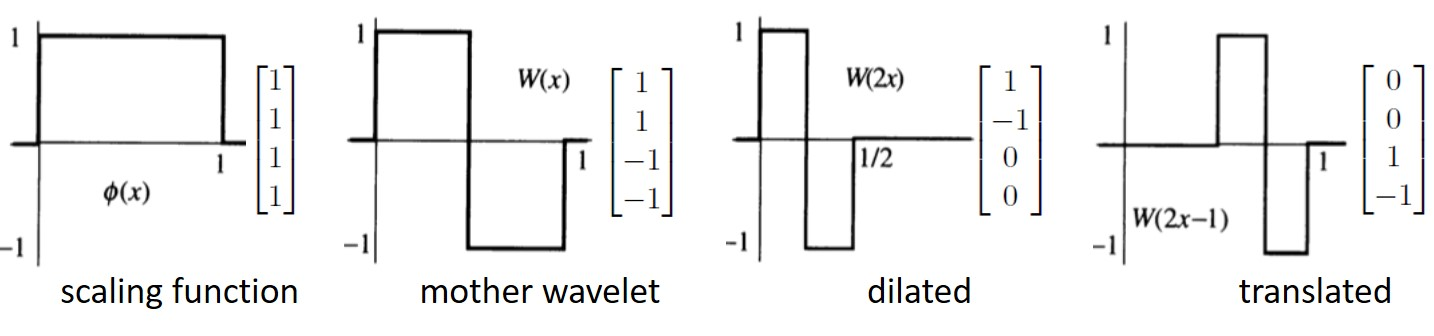
\includegraphics[width=12.5cm]{fig_9_6.jpg} 
	\caption{4-dimension Haar wavelets.}\label{fig_9_6}
\end{figure}
\par Here another important family of orthonormal basis comes into play for these local cases, the wavelets. Take the 4-dimension Haar wavelets as an example (Figure \ref{fig_9_6}). Haar wavelets construct basis consisting of a scaling function (averaging), a mother wavelet that detects changes by contrasting the first and the second half, and some dilated and/or translated mother wavelet. Note that they need to be normalized to form an orthonormal basis. For $D=4$ we get the following orthonormal matrix
\begin{equation*}
	{\bf U}=\frac{1}{2}\begin{pmatrix}
	1&1&\sqrt{2}&0\\
	1&1&-\sqrt{2}&0\\
	1&-1&0&\sqrt{2}\\
	1&-1&0&-\sqrt{2}
	\end{pmatrix}.
\end{equation*}
For $D=8$ we have
\begin{equation*}
{\bf U}=\frac{1}{2}\begin{pmatrix}
1&1&\sqrt{2}&0&2&0&0&0\\
1&1&\sqrt{2}&0&-2&0&0&0\\
1&1&-\sqrt{2}&0&0&2&0&0\\
1&1&-\sqrt{2}&0&0&-2&0&0\\
1&-1&0&\sqrt{2}&0&0&2&0\\
1&-1&0&\sqrt{2}&0&0&-2&0\\
1&-1&0&-\sqrt{2}&0&0&0&2\\
1&-1&0&-\sqrt{2}&0&0&0&-2
\end{pmatrix}.
\end{equation*}
Actually for $D=2^n$ we can keep doing dilation and translation with normalization to form the Haar wavelets. Wavelets can be regarded as little finite supported local time domain filters, and can take other shape with basis generated also by dilation and translation (Figure \ref{fig_9_7}).
\begin{figure}[h] 
	\centering 
	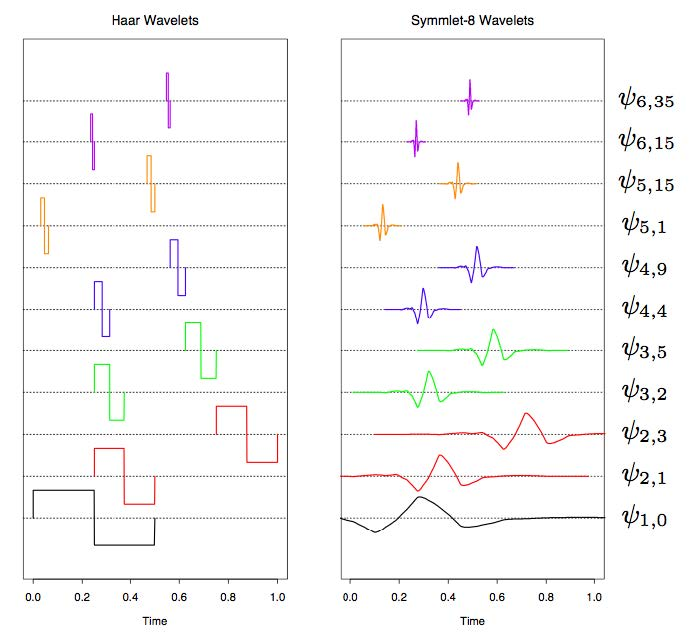
\includegraphics[width=8cm]{fig_9_7.jpg} 
	\caption{Other wavelets.}\label{fig_9_7}
\end{figure}
Using DWT (left of Figure \ref{fig_9_8}) we can construct a denoised localized signal. Also if we apply DWT to the signal in Figure \ref{fig_9_2} we get the right part of Figure \ref{fig_9_8}. Although the reconstruction is not as smooth as the one produced by DFT, it is still good. The pulses appears because of the localized property of wavelet since if something is strong enough locally, wavelets will think there is something interesting happening and captures that. 
\begin{figure}[h] 
	\centering 
	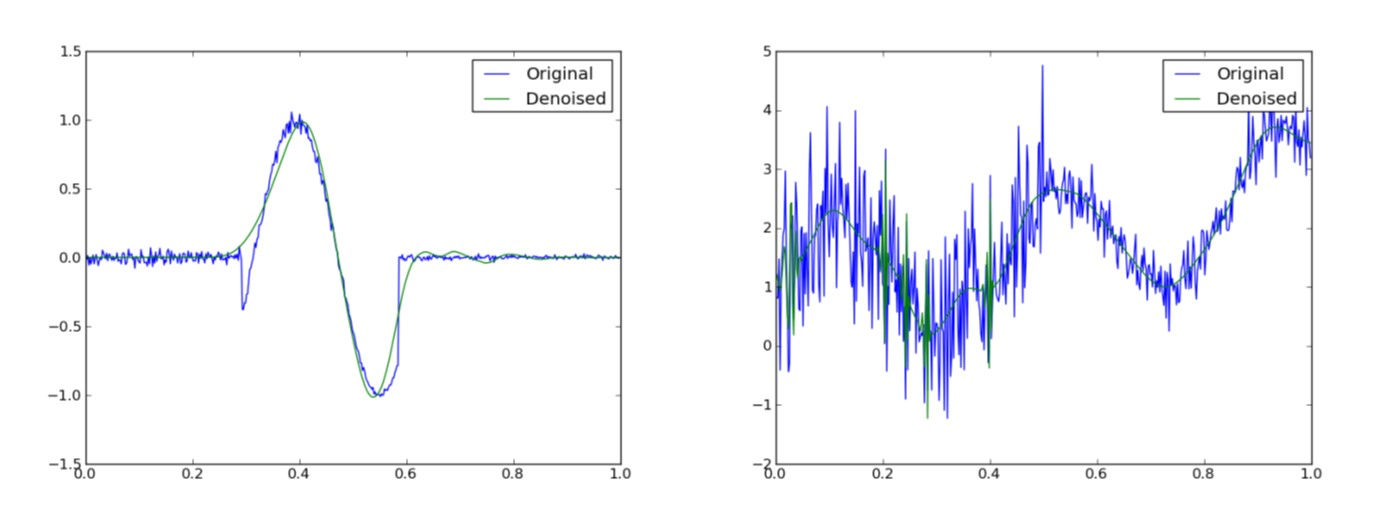
\includegraphics[width=12cm]{fig_9_8.jpg} 
	\caption{Left: DWT for localized signal. Right: DWT for signal in Figure \ref{fig_9_2}.}\label{fig_9_8}
\end{figure}
\par There does not exist a choice of a transform that is better than all other choices. It depends on the signal type. The Fourier basis has global support and is good for ``sine-like'' signals, while is poor for localized signals. The wavelet basis, on the contrast, has local support and is good for localized signals while is poor for non-banishing signals. In practice, it turns out to be very tricky for picking a proper basis and choose a proper threshold $\epsilon$. 
\subsection{Connection with PCA}
Now we look back to PCA and see how we can connect it to sparse coding. For a PCA setting, usually we are given a set of data/signal ${\bf X}=[{\bf x}_1,\dots,{\bf x}_N],\ {\bf x}_i\in \mathbb{R}^D$. The first step is to compute the mean $\bar{\bf x}=\frac{1}{N}\sum_{n=1}^{N}{\bf x}_n$. Then we can compute the centered covariance matrix by
\begin{equation*}
	{\bf \Sigma}=\frac{1}{N}({\bf X-M})({\bf X-M})^T,\quad {\bf M}:=[\underbrace{\bar{\bf x},\dots,\bar{\bf x}}_{N\text{ times}}].
\end{equation*}
The next step is to perform the eigen-decomposition for ${\bf \Sigma}$:
\begin{equation*}
	{\bf \Sigma}={\bf U\Lambda U}^T,
\end{equation*}
where by construction ${\bf \Sigma}$ is a real symmetric positive semidefinite (p.s.d.) matrix and ${\bf U}$ is orthonormal. The eigenvalues are order in $\lambda_1\geq \lambda_2\geq \cdots\geq \lambda_D\geq 0$, where the non-negativity is by p.s.d.. PCA is complete by ``throwing away'' the $D-K$ directions with smallest variance (note that this depends on the whole data set, not individual signal). If we think of this as a sparsification, this is equivalently to keep the $K$ largest eigenvectors:
\begin{equation*}
	\hat{\bf x}={\bf U}\hat{\bf z},\quad \hat{z}_d = \begin{cases}
	z_d&\ {\rm if}\ d\leq K\\
	0&\ {\rm otherwise}
	\end{cases}.
\end{equation*}
With ordered eigenvalues, it suffices to define ${\bf U}_k$ as
\begin{equation*}
	{\bf U}_K:=[{\bf u}_1,\dots,{\bf u}_K]
\end{equation*}
and to reconstruct via
\begin{equation*}
	\hat{\bf x}={\bf U}_K{\bf z}_{[1:K]}.
\end{equation*}
Note that the selection process of PCA is a little bit different from things we have done before. Here we are not thresholding or selecting the coefficients of a given signal ${\bf x}$ but selecting in terms of $\lambda$'s that are obtained based on the whole data set. Therefore PCA differs from DFT and DWT in the sense that it construct a data driven dictionary, where we have to start with samples to determine the orthonormal transformation ${\bf U}$, while the DFT and DWT apply domain knowledge and can be defined beforehand.
\par In terms of signal processing or communication, for the PCA basis
\begin{itemize}
	\item ${\bf U}_K$ is data-dependent, optimal for given ${\bf \Sigma}$ in terms of reconstruction error;
	\item the sender needs to transmit the eigenvectors (basis) $\{{\bf u}_d:d\leq K\}$ and the corresponding coding ${\bf z}_{1:K}$.
\end{itemize}
For the fixed basis
\begin{itemize}
	\item the sender and receiver agree on basis beforehand, e.g. Haar Wavelets;
	\item the sender only have to transmit the non-zero elements of $\hat{\bf z}$.
\end{itemize}
\subsection{Image Compression}
To close up this section, we now take a look at the image compression. We start with 2-D Discrete Cosine Transform (DCT), which is used in JPEG. For compression, DCT first break a big image into $8\times 8$ blocks and applies 64 basis functions to each block. Figure \ref{fig_9_9} shows how these basis functions look like. To understand the figure, think of each $8\times 8$ patches as a $D=64$ vector, then the basis functions are also $D=64$ vectors which can also be represent as $8\times 8$ patches. Since there are 64 basis functions in total we can arrange them on a $8\times 8$ grid, with each red square is a basis function. Due to the image cutting or breaking step, DCT suffers from some boundary effects. There are other more sophisticated basis functions that can do overlapping and give visually better results.
\begin{figure}[h] 
	\centering 
	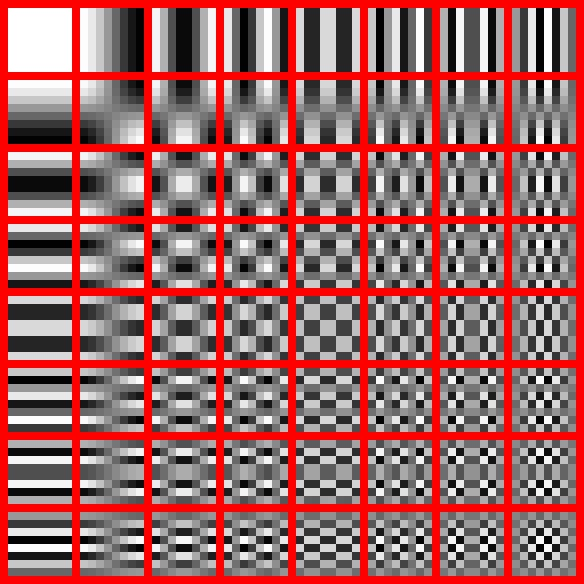
\includegraphics[width=4cm]{fig_9_9.jpg} 
	\caption{DCT basis.}\label{fig_9_9}
\end{figure}
\begin{figure}[h] 
	\centering 
	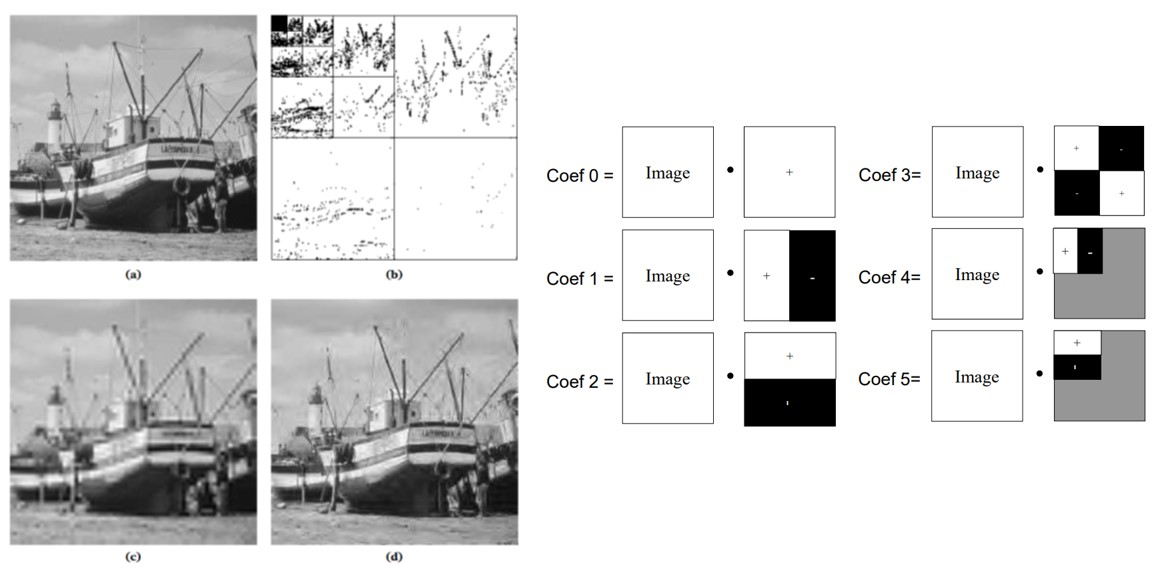
\includegraphics[width=12.5cm]{fig_9_10.jpg} 
	\caption{(Left) Image compression with wavelets: (a) Discrete image of $256^2$ pixels; (b) orthonormal wavelet coefficients at 4 different scales with black points correspond to large coefficients; (c) Approximation using the three largest scales; (d) Approximation using the $K$ largest coefficients ($K=\frac{256^2}{16}$). (Right) Definition of the first few (coarsest scale) wavelet coefficients of an image.}\label{fig_9_10}
\end{figure}
\begin{figure}[h] 
	\centering 
	\includegraphics[width=10cm]{fig_9_2D_wavelet.jpg} 
	\caption{Illustration of how the wavelet coefficients are arranged to form a pyramid. Left: each large block corresponds to a basis/filter and will be element-multiplied with the image to give an coefficient. Right: The way we arrange coefficients with different row/column frequencies to form the coefficient pyramid.}\label{fig_9_2D_wavelet}
\end{figure}
\par Wavelets turn out to be another successful way to compress images. Given an image shown in (a) of the left part of Figure \ref{fig_9_10}, we can compute the corresponding wavelet coefficients ((b) in the left of Figure \ref{fig_9_10}) and use them to construct approximations ((c) and (d)). The visualization of wavelets for images is often in this multiresolution representation. To understand this visualization, we can take a look at the right of Figure \ref{fig_9_10}\footnote{From https://www.cs.toronto.edu/~mangas/teaching/320/slides/CSC320L11.pdf
}. The first coefficient is just the average of all points corresponding to the most top-left block in (b). Then we apply the mother wavelet horizontally and vertically resulting in coefficients 1 to 3, corresponding to the 3 blocks (in the same size) around the top-left black block in (b). Then we do dilation and translation to generate more coefficients (Figure \ref{fig_9_2D_wavelet}). Note that as the basis function becoming more and more localized, it gains the ability to capture things with higher and higher frequency with, at the same time, larger and larger number of coefficients in the same scale (rearranging things gives the pyramid visualization results in (b)). (c) shows an approximation using only the coefficients in the three largest scales, which can be regarded as a low-pass filtering. In (d) we are more selective about where to keep the coefficients. Since most of parts in high-frequency coefficients are zeros, by throwing away small ones, we get a compression while keeping both the low-frequency properties as well as high-frequency things for important locations. Wavelets for its robustness with noise are also used for image denoising (for example see the slides).
\par Figure \ref{fig_9_11} shows an example for different compression algorithms. We see the mosaic-like things caused by DCT used in JPEG, while the wavelets produces better results with the same compression ratio. Note that wavelet other than Haar wavelet is used here.
\begin{figure}[h] 
	\centering 
	\includegraphics[width=12.5cm]{fig_9_11.jpg} 
	\caption{Results from different compression algorithms. JPEG: DCT; JPEG2000: wavelets.}\label{fig_9_11}
\end{figure}
One last thing to mention when it comes to image compression is the computational efficiency. Naively apply basis transformation ia matrix multiplication yield a $O(D^2)$ cost, where $D$ is the number of pixels in a image, and this can be gigantic. The way in practice we compute the transformation is not by explicitly instantiating the ${\bf U}$ matrix and doing multiplications, but by exploiting fast transforms:
\begin{itemize}
	\item Fourier: $O(D\log D)$
	\item Wavelet: $O(D)$ or $O(D\log D)$.
\end{itemize}
Another natural way to relieve this problem is by breaking up images into blocks, and transform each block. This avoids quadratic blow-up, but as shown in Figure \ref{fig_9_11} sacrifices perceptual qualities.
\section{Overcomplete Dictionaries}
In this section, however, we want to go beyond the orthonormal transforms and see how this can benefit sparsity representation. So far, based on the assumption that natural signals have approximate sparse representation in suitable orthonormal bases, e.g. wavelets for natural images, we have done a lot of things. Briefly speaking, in the coding via orthonormal transforms we do the following
\begin{itemize}
	\item given: signal ${\bf x}$ and orthonormal matrix ${\bf U}$
	\item compute linear transformation (change of basis) ${\bf z}-{\bf U}^T{\bf x}$
	\item truncate ``small'' values, ${\bf z}\mapsto \hat{\bf z}$
	\item compute inverse transform (recall ${\bf U}^{-1}={\bf U}^T$) $\hat{\bf x}={\bf U}\hat{\bf z}$.
\end{itemize}
The quality of reconstruction is measured by the error $\|{\bf x-}\hat{\bf x}\|^2$, and when we have a small error, we find a sparse coding vector $\hat{\bf z}$. Recall that for dictionary choice, the Fourier dictionary is good for ``sine like'' signals, while a wavelet dictionary is good for localized signals. As mentioned before, choosing a proper basis is hard in practice, so one natural thing to ask is why not just use a combination of these families of basis and just figure out which one is right after we have encoded the signal. This motivates the more general dictionaries we are going to talk about: overcomplete dictionaries. Actually, in terms of reconstruction, we don't need $>N$ atoms for signals in $\mathbb{R}^N$, but as we will see, in terms of sparsity, this setting is feasible and makes sense.
\par The idea of overcomplete dictionaries, motivated by that no single basis is optimally sparse for all signal classes, is really to exploit the overcompleteness (${\bf U}^{D\times L}$ such that $L>D$), which means we use more atoms (dictionary elements) than dimensions. Now the problem comes to how we can construct this dictionary, and with it how can we decode/reconstruct signals. Briefly speaking, we union orthonormal bases to generate overcomplete dictionaries, and use some coding algorithm to choose the best representation. Note that choosing the best representation is little bit more involved since by construction we can find multiple coding that can do the exact recovery due to the redundancy of representation.
\subsection{Encoding (Dictionaries)}
For constructing the dictionaries, the strategy is really to do it manually by signal inspection (looking at the signal and see what interesting properties does it have). We can simply try several and choose the one which affords the sparest coding. 
\par Here is one inspiring example from S. Mallat, A Wavelet Tour of Signal Processing – The Sparse Way, Academic Press, 2009. As shown in Figure \ref{fig_9_12}, signal might be a superposition of several characteristics, say smooth gradients and oscillating textures. Since a single orthonormal basis cannot sparsely code both, like wavelet basis might be good at the smooth gradient part while fails to captures the high-frequency texture part. The idea of building the dictionary is then to use algorithms to pick atoms (dictionary elements) from a union of bases, each one responsible for on characteristic.
\begin{figure}[h] 
	\centering 
	\includegraphics[width=12.5cm]{fig_9_12.jpg} 
	\caption{Signal might be a superposition of several characteristics.}\label{fig_9_12}
\end{figure}
\par As an example for capturing the oscillating texture, we introduce the following Gabor wavelets, which is directional oscillation with its amplitude modulated by a Gaussian window
\begin{align*}
	g(n_1,n_2;\mu_1,\mu_2,f,\theta)&\propto \exp[-(n_1-\mu_1)^2]\exp[-(n_2-\mu_2)^2]\\
	&\times\cos(f\cdot(n_1\cos \theta+n_2\sin\theta)).
\end{align*}
Figure \ref{fig_9_13} shows some examples of Gabor wavelets with different settings. The size of the dictionary size is determined by the discretizing parameter range of $\mu_1,\mu_2,f$ and $\theta$.
\begin{figure}[h] 
	\centering 
	\includegraphics[width=12.5cm]{fig_9_13.jpg} 
	\caption{Examples of Gabor wavelets.}\label{fig_9_13}
\end{figure}
\par The following example gives some intuition about how general overcomplete dictionaries can benefit sparsity. Consider data set $\{{\bf x}_1,\dots,{\bf x}_{10000}\}\in \mathbb{R}^3$ as shown in Figure \ref{fig_9_14}, where data points mainly lie in 2 intersecting hyperplanes. (Actually I am not sure if this explains Figure \ref{fig_9_14}.)
\begin{figure}[h] 
	\centering 
	\includegraphics[width=5cm]{fig_9_14.jpg} 
	\caption{Visualization of the data set.}\label{fig_9_14}
\end{figure}
\par The full coding needs $(K=3)$ in spanning basis ${\bf U}\in \mathbb{R}^{3\times 3}$ to give accurate reconstruction. However, a $K=2$ coding with small error is possible using a four atom dictionary
\begin{equation*}
	\tilde{\bf U}=[{\bf u}_1,{\bf u}_2,{\bf u}_3,{\bf u}_4]\in \mathbb{R}^{3\times 4},
\end{equation*}
where $[{\bf u}_1,{\bf u}_2]$ are the bases for the first hyperplane, while $[{\bf u}_3,{\bf u}_4]$ are the bases for the second hyperplane. 
\par Note that $L>D$ means the atoms are no longer linearly independent. We can define the overcompleteness by factor $\frac{L}{D}$, which also indicates the dictionary size. Increasing $\frac{L}{D}$ potentially increases the sparsity of the coding (we hope), while increases the linear dependency between atoms. If we have a very large $L/D$ there might even have several groups of atoms form the same subspace.
In this case we would like to have a way to measure the redundancy other than simply count the number of atoms by $\frac{L}{D}$. A way to do this is via a linear dependency measure for dictionaries: coherence, which is defined by 
\begin{equation*}
	m({\bf U})=\max_{i,j:i\neq j}|{\bf u}_i^T{\bf u}_j|,
\end{equation*}
where we have $m({\bf B})=0$ for an orthonormal basis ${\bf B}$, and $m([{\bf B}\ {\bf u}])\geq \frac{1}{\sqrt{D}}$ if atom ${\bf u}$ is added to an orthonormal ${\bf B}$ (consider $1=\sum_i u_i^2\leq D u_{max}^2$).  
\subsection{Signal Reconstruction}
The main point to have this measurement comes from the hardness of finding the best/sparsest representation due to the redundancy in the dictionary. If we naively compute the coding ${\bf z}$ via ${\bf z} = {\bf U}^T{\bf x}$, 
for orthonormal ${\bf U}$ this is okay, we can simply compute ${\bf x}={\bf Uz}$. Even for cases that ${\bf U}$ is a spanning bases ($D$ linearly independent atoms), the reconstruction can be problematic, in a sense that in
\begin{equation*}
	{\bf x} = ({\bf U}^T)^{-1}{\bf z},
\end{equation*}
inverting ${\bf U}^T$ can be ill-conditioned. To understand the word ``ill-conditioned'', considering the following example where
\begin{equation*}
	{\bf U}^T=\frac{1}{2}\begin{bmatrix}
	1&1\\
	1+10^{-10}&1-10^{-10}
	\end{bmatrix}
	,\quad ({\bf U}^T)^{-1}=\begin{bmatrix}
	1-10^{10}&10^{10}\\
	1+10^{10}&-10^{10}
	\end{bmatrix}.
\end{equation*}
This can be problematic, since a tiny distortion in ${\bf z}$ (caused by say some noise) will completely change the reconstructed ${\bf x}$ for the large elements in the inverse transform. For general dictionaries, where ${\bf U}\in\mathbb{R}^{D\times L}$ is overcomplete (L>D), finding the best representation ${\bf z}$ in terms of reconstruction error is ill-posed due to the redundancy in the dictionary. But if we say that the sparsity is the main thing that we care about, by adding a constraint: find the sparest ${\bf z}\in \mathbb{R}^L$ such that ${\bf x}={\bf Uz}$, the problem is now mathematically solvable. Formally, we now try to solve a problem given by
\begin{align}
	\label{eq_9_L0}&{\bf z}^*\in\mathop{\arg\min}_{\bf z}\|{\bf z}\|_0\\
	&{\rm s.t.}\quad {\bf x}={\bf Uz},\notag
\end{align}
where $\|{\bf z}\|_0$ counts the number of non-zero elements in ${\bf z}$. This means we want to find the sparest solution, under the equality constraint. However, this is in general a NP-hard combinatorial problem. To directly solve the problem, we can either try brute-force: exhaustive search over all atom subsets (exponential in $L$), or we can use some greedy approach, e.g. Matching Pursuit (Mallat \& Zhang 1993), which is to do the following:
\begin{itemize}
	\item assume (length) normalized atoms ${\bf u}_j$
	\item greedily select $j^*=\arg\max_j|\langle {\bf x},{\bf u}_j\rangle|$
	\item add $\hat{\bf x}\leftarrow \hat{\bf x} + \langle {\bf x},{\bf u}_{j^*}\rangle {\bf u}_{j^*}$, where $\hat{\bf x}$ is the reconstruction
	\item compute residual ${\bf x}\leftarrow {\bf x} - \langle {\bf x},{\bf u}_{j^*}\rangle {\bf u}_{j^*}$
	\item repeat until some condition is satisfied.
\end{itemize}
Note that just as many other greedy approach, matching pursuit has no guarantee to find the best representation in general. Another way that are better understood theoretically is to change the problem into a convex optimization task. Specifically, we change the objective from minimizing the $L_0$ norm to $L_1$ norm:
\begin{align}
	\label{eq_9_L1}&{\bf z}^*\in\mathop{\arg\min}_{\bf z}\|{\bf z}\|_1\\
&{\rm s.t.}\quad {\bf x}={\bf Uz}.\notag
\end{align}
This convex optimization problem can be solved efficiently, and under suitable conditions on ${\bf U}$, the solution of the two problems are equivalent.
\subsection{Sparsity and Exact recovery}\label{sec_9_comp_sens}
We conclude this chapter with some supplementary materials from one of my favorite courses at ETH, Mathematics of Data Science by Prof. Afonso S. Bandeira. This subsection is again totally out of the scope of CIL, but since it is rather relevant I put it here. Feel free to skip!
\par Assuming that ${\bf x}$ has a sparse coding under a overcomplete dictionary ${\bf U}$, in order for (\ref{eq_9_L1}) to be a good procedure for sparse recovery (\ref{eq_9_L0}) we need two things:
\begin{enumerate}
	\item the solution of (\ref{eq_9_L1}) is meaningful for (\ref{eq_9_L0}) (hopefully to be the same)
	\item the solution of (\ref{eq_9_L1}) can be efficiently found.
\end{enumerate}
We first take a look at the second one. Let $\bm{\omega}^+$ and $\bm{\omega}^-$ be the positive part and the symmetric negative part of ${\bf z}$, meaning that ${\bf z}=\bm{\omega}^+ - \bm{\omega}^-,\ \bm{\omega}^+\geq {\bf 0},\ \bm{\omega}^-\geq {\bf 0}$ and, for each $i$, either $\omega_i^+$ or $\omega_i^-$ is zero. In this case, we have
\begin{equation*}
	\|{\bf z}\|_1=\sum_i \omega_i^+ + \omega_i^- = {\bf 1}^T(\bm{\omega}^+ + \bm{\omega}^-).
\end{equation*}
Then we consider a linear programming given by
\begin{align}
	\label{eq_9_lp}\min_{\bm{\omega}^+ , \bm{\omega}^-}\ &{\bf 1}^T(\bm{\omega}^+ + \bm{\omega}^-)\\
	{\rm s.t.}\ &{\bf U}(\bm{\omega}^+ - \bm{\omega}^-) = {\bf x}\notag\\
				& \bm{\omega}^+\geq {\bf 0}\notag\\ 
				&\bm{\omega}^-\geq {\bf 0}.\notag
\end{align}
The optimal solution of (\ref{eq_9_lp}) will satisfy that for each $i$, either $\omega_i^+$ or $\omega_i^-$ is zero since if it is not satisfied, we can reduce the part where both $\omega_i^+$ and $\omega_i^-$ are greater than 0 and decrease the objective. Therefore solving (\ref{eq_9_L1}) is equivalent to solve a linear programming (\ref{eq_9_lp}) which is efficiently solvable. 
\par For the first requirement, recall our assumption that ${\bf x}$ has a sparse coding ${\bf z}^*$. Formally we require ${\bf z}^*$ to be $s$-sparse, i.e. $\|{\bf z}^*\|_0\leq s$. Let's consider when will ${\bf z}^*$ fail to be the unique optimal solution for the $L_1$ minimization problem (\ref{eq_9_L1}).
\par Let $S={\rm supp}({\bf z}^*)$ (the support of ${\bf z}^*$, i.e. the set of indexes of non-zero entries) and $|S|=s$. If ${\bf z}^*$ is not the unique optimal solution for (\ref{eq_9_L1}), there exists a non-zero vector ${\bf v}$ such that ${\bf z^*+v}$ is an optimal solution. This means
\begin{equation*}
	\|{\bf z^*+v}\|_1\leq \|{\bf z}^*\|_1,\text{ and }{\bf U(z^*+v)}={\bf x},
\end{equation*}
which means ${\bf Uv}=0$. Also,
\begin{equation*}
	\|{\bf z}^*_S\|_1 = \|{\bf z}^*\|_1 \geq \|{\bf z^*+v}\|_1 = 	\|({\bf z^*+v})_S\|_1 + \|{\bf v}_{S^c}\|_1 \geq \|{\bf z}^*_S\|_1 - \|{\bf v}_S\|_1 + \|{\bf v}_{S^c}\|_1,
\end{equation*}
where the subscript $S$ means restricting elements to $S$. This means if ${\bf z}^*$ is not the unique optimal solution for the $L_1$ minimization problem, there must exist some non-zero vector ${\bf v}$ in the kernel of ${\bf U}$, such that $\|{\bf v}_S\|_1\geq \|{\bf v}_{S^c}\|_1$. Since that $|S|\ll L$, it is unlikely for ${\bf U}$ to have vectors in its nullspace that are so concentrated on such few entries. This motivates the following definition.
\begin{definition}
	(Null Space Property) ${\bf U}$ is said to satisfy the $s$-Null Space Property (${\bf U}\in s$-NSP) if, for all ${\bf v}$ in ${\rm ker}({\bf U})$ (the nullspace of ${\bf U}$) and all $|S|=s$, we have
	\begin{equation*}
		\|{\bf v}_{S}\|_1<\|{\bf v}_{S^c}\|_1.
	\end{equation*}
\end{definition}
We see that by construction, if our overcomplete dictionary matrix ${\bf U}$ satisfies the Null Space Property for $s$, then for a ${\bf x}$ with a $s$-sparse coding ${\bf z}^*$, ${\bf z}^*$ will be indeed the optimal solution to (\ref{eq_9_L1}), which means with ${\bf U}$ it finds the best coding for any signal with a $s$-sparse coding.
\par There are many other properties leading to the coincidence of the solution to the $L_1$ minimization problem and the $L_0$ problem. A particularly useful one is the Restricted Isometry Property (RIP) defined by
\begin{definition}\label{def_9_RIP}
	(Restricted Isometry Property (RIP)) An $m\times p$ matrix $U$ is said to satisfy the $(s,\delta)$-Restricted Isometry Property (RIP) if 
	\begin{equation*}
		(1-\delta)\|z\|^2\leq \|Uz\|^2\leq (1+\delta)\|z\|^2
	\end{equation*}
	holds for all $s$-sparse $z$.
\end{definition}
RIP describes the property of approximately preserving the length of sparse vectors. The following theorem connects RIP to our topic
\begin{theorem}\label{thm_9_RIP}
	Let $x=Uz^*$ where $z^*$ is an s-sparse vector. Assume that $U$ satisfies the RIP with $\delta_{2s}<\frac{1}{3}$, then the solution $z_0$ to the $L_1$ minimization problem
	\begin{equation*}
		min_z \|z\|_1,\ s.t.\ Uz=x=Uz^*
	\end{equation*}
	becomes $z^*$ exactly, i.e. $z_0=z^*$.
\end{theorem}
The point to introduce RIP is to give some insight about how coherence that measures the redundancy of dictionary ${\bf U}$ can affect our coding. Recall the definition of (worst-case) coherence
\begin{equation*}
	\mu:=m({\bf U})=\max_{i\neq j}\|{\bf u}_i^T{\bf u}_j\|.
\end{equation*}
Given a dictionary ${\bf U}$ with unit-length atoms and worst-case coherence $\mu$, then it has been proved that ${\bf U}$ will satisfies $(s,\mu(s-1))$-RIP meaning that it will be $(s,\frac{1}{3})$-RIP for $s\leq \frac{1}{3\mu}$. By theorem \ref{thm_9_RIP}, when $s\leq \frac{1}{3\mu}$, with dictionary ${\bf U}$ we can efficiently find the best sparse representation for all signals that for which there exists such $s$-sparse representation ${\bf z}^*$. This motivates the problem of designing dictionaries with smallest possible worst-case coherence. This is a central problem in Frame Theory.

%%%%%%%%%%%%%%%%%%%%%%%%%%%%%%%%%%%%%%%%%%%%%%%%%%%%%%%
%   New Chapter                                       %
%%%%%%%%%%%%%%%%%%%%%%%%%%%%%%%%%%%%%%%%%%%%%%%%%%%%%%%

\chapter{Dictionary Learning}
In the last chapter, we talked about finding better representations for data in terms of sparsity, where for a signal its representation can be in a high dimensional space but with only a few entries non-zero. In this chapter, we will explore the following idea: instead of manually choosing bases like wavelets or Fourier basis, can we somehow learn a good dictionary based on some given data? Our discussion will start with a brief introduction to Compressive sensing, which as mentioned in section \ref{sec_9_comp_sens} belongs to this context of sparseness. We will then talk about how to conduct dictionary learning in terms of matrix factorization, specifically with K-SVD algorithm.
\section{Compressive Sensing}
Recall our assumption that many types of signal/data are sparse in certain basis. What we have done in the last chapter is to transform such signals with proper ${\bf U}$, and then we can efficiently transmit data in their sparse coding given both the sender and receiver having the same dictionary. This means that when we take a picture, our camera first measure all the pixels, but after an appropriate change of basis we ``throw away'' most of them. This sounds rather wasteful. The natural question raises is: if only a few degree of freedom are needed for representing the data, why not measuring the data in a more efficient way, where we take considerably less measurements than the number of pixels. 
\par This idea is really at the heart of compressive sensing, and it is of great importance in the sense that it decreases acquisition time, power assumption and required storage. For an example, think about photoshooting in space. It saves memory and battery power if fewer measurements is required for taking a picture. For another important application for compressive sensing, high-resolution MRI images require patients to be perfectly still during the scanning. Decreasing the number of measurements with compressive sensing can significantly reduce the scanning time saving the energy consumption and causing less damage to the patients.
\par To build the concept, consider the original signal denoted by ${\bf x}\in \mathbb{R}^D$ which is $K$-sparse in orthonormal basis ${\bf U}\in\mathbb{R}^{D\times D}$:
\begin{equation*}
	{\bf x}={\bf Uz},\quad {\rm s.t.}\quad \|{\bf z}\|_0=K.
\end{equation*}
The idea is to acquire set ${\bf y}$ of $M$ linear combinations of the signal, like instead of measuring all pixels in an image, we somehow only compute a few linear combinations of all pixels, and hopefully these measurements (linear features) can be used to reconstruct the original signal. Formally, we have
\begin{align*}
	&y_k=\langle {\bf w}_k,{\bf x}\rangle,\quad k=1,\dots,M\\
	&{\bf y}={\bf Wx}={\bf WUz}=:{\bf \Theta z},\ {\rm with}\ {\bf \Theta}={\bf WU}\in\mathbb{R}^{M\times D}.
\end{align*}
If $M\ll D$, the measured signal ${\bf y}$ will be much shorter than ${\bf x}$, though we have to require that with it we are able to reconstruct the signal (see Figure \ref{fig_10_1} for a visualization of these matrices).
\begin{figure}[h] 
	\centering 
	\includegraphics[width=10cm]{fig_10_1.jpg} 
	\caption{A visualization of the idea behind compressive sensing.}\label{fig_10_1}
\end{figure}
\par One might ask, under what condition will it be possible to reconstruct the signal ${\bf x}$ (equivalent to require reconstruction for ${\bf z}$ since given ${\bf U}$ we have ${\bf x}={\bf Uz}$). Surprisingly given any orthonormal basis ${\bf U}$ we can obtain a stable reconstruction for any $K$-sparse compressible signal, if we choose ${\bf W}$ to be a Gaussian random projection, i.e. $w_{ij}\sim \mathcal{N}(0,\frac{1}{D})$ with $M\geq cK\log(\frac{D}{K})$, where $c$ is some constant. Note that the dimension $D$ has only log effects.
\begin{remark}
	Since ${\bf U}$ is an orthonormal matrix, ${\bf \Theta}={\bf WU}$ will remain a Gaussian random projection. It can be shown that there exists a constant $c$ such that if
	\begin{equation*}
		M\geq cK\log(\frac{D}{K}),
	\end{equation*}
	then ${\bf \Theta}$ (a Gaussian random projection) satisfies the $(K,\frac{1}{3})$-RIP (Definition \ref{def_9_RIP}) with high probability. Then with theorem \ref{thm_9_RIP}, we can reconstruct any sparse vector by solving the $L_1$ minimizing problem:
	\begin{equation*}
		\min \|{\bf z}\|_1,\ {\rm s.t.}\ {\bf y}={\bf \Theta z}.
	\end{equation*}
\end{remark}
As mentioned, recovering ${\bf x}$ is equivalent to find ${\bf z}$ which is $K$-sparse. Again we see it is an ill-posed problem since there are more unknowns than equations ($M\ll D$). Note that here the problem does not raise from the overcompleteness but from the sensing matrix by design. We can again require constraints on sparseness to make it a proper optimization problem, where we try to solve
\begin{equation*}
	{\bf z}^*\in \mathop{\arg\min}_{\bf z}\|{\bf z}\|_0,\ \text{s.t. }{\bf y}={\bf \Theta z}.
\end{equation*} 
We can apply the same reconstruction techniques as before: (1) convex optimization (use a surrogate $\|\cdot\|_1$ instead) or (2) Matching Pursuit.
\section{Dictionary Learning}
Now let's move on to the topic of dictionary learning. In all previous cases including compressive sensing, we always assume the transform matrix ${\bf U}$ is known. But can we work with better and more problem specific dictionaries? Recall the fixed orthonormal basis setting:
\begin{equation*}
	{\bf x} = \underbrace{U}_{D\times D}\cdot {\bf z},
\end{equation*}
where we benefit from the efficient inversion of ${\bf U}$: ${\bf z} = {\bf U}^T{\bf x}$, while as a strong priori assumption one ${\bf U}$ usually only works for specific classes of signals; for the oversampling basis setting:
\begin{equation*}
{\bf x} = \underbrace{U}_{D\times L}\cdot {\bf z},\ L>D,
\end{equation*}
we can have sparse coding for several signal classes (or classes with mixture of characteristics), but finding such the sparsest coding may require approximation algorithms (e.g. matching pursuit) and can be problematic if dictionary size $L$ and coherence $m(\bf U)$ are large. The advantage of learning is that we can adapt a dictionary to signal characteristics of the given data set resulting in the same approximation error achievable with smaller $L$.
\subsection{Basic Idea}
To learn a dictionary, first assume we are given a set of images/data (data set).  The idea is to write the transform in a matrix form giving the following matrix factorization problem
\begin{equation}
	\underbrace{\bf X}_{D\times N}\approx \underbrace{\bf U}_{D\times L}\cdot \underbrace{\bf Z}_{L\times N},
\end{equation} 
where ${\bf X}=[{\bf x}_1,\dots,{\bf x}_N]$ is the data matrix, ${\bf U}=[{\bf u}_1,\dots,{\bf u}_L]$ is the dictionary matrix, and ${\bf Z}=[{\bf z}_1,\dots,{\bf z}_N]$. As a dictionary learning problem, we also require constrains further constraints on:
\begin{itemize}
	\item ${\bf U}$: columns/atoms are norm-normalized
	\item ${\bf Z}$: the coding ${\bf z}_i$ should be sparse.
\end{itemize}
Before we move to how we can solve this rather scaring problem, let's first take a look at how can we banefit from this adaptive dictionary. Figure \ref{fig_10_2} shows an example of dictionary learning for $8\times 8$ pixel image patches of face images. We see that the learned dictionary looks quite different from the fixed ones in the sense of randomness. However, they share some similarities as in the learned dictionary there are many atoms seems like edge detectors (but in some different directions).
\begin{figure}[h] 
	\centering 
	\includegraphics[width=10cm]{fig_10_2.jpg} 
	\caption{Example of dictionary learning from M. Aharon et al. 2006}\label{fig_10_2}
\end{figure}
\par Dictionary learning can also be used for image inpainting, where we are given an image with a mask indicating where it is missing, and we need to complete the image. The idea is really that, a dictionary will do better in inpainting if it's more adapted to the signal. We can construct a sparse coding of observed pixels and predict missing pixels from the sparse code (in some sense similar to denoising).
\begin{figure}[h] 
	\centering 
	\includegraphics[width=8cm]{fig_10_3.jpg} 
	\caption{Image inpainting (from the internet).}\label{fig_10_3}
\end{figure}
\subsection{Matrix Factorization and K-SVD}
Formally speaking, learning a dictionary with corresponding coding for a given data set ${\bf X}$ is to solve the following matrix factorization problem
\begin{equation*}
	({\bf U^*,Z^*})\in \mathop{\arg\min}_{{\bf U,Z}}\|{\bf X}-UZ\|^2_F,
\end{equation*}
where $\|\cdot\|_F$ is the Frobenius norm defined by $\|{\bf A}\|_F^2=\sum_{i,j}a_{ij}^2$. The hardness comes from that the objective is not jointly convex in ${\bf U}$ and ${\bf Z}$, and different from the situation we have faced, it is not even convex in either ${\bf U}$ and ${\bf Z}$ given that the columns of ${\bf Z}$ are sparse and atoms of ${\bf U}$ are normalized. Still, we can try a iterative greedy minimization:
\begin{enumerate}
	\item \textbf{Coding step:} With fixed dictionary ${\bf U}$ we update the coding matrix via
	\begin{equation}\label{eq_10_obj_coding}
		{\bf Z}^{t+1}\in \mathop{\arg\min}_{\bf Z} \|{\bf X}-{\bf U}^t{\bf Z}\|_F^2,
	\end{equation}
	subject to ${\bf Z}$ being sparse (non-convex constraint).
	\item \textbf{Dictionary update step:} We update the dictionary via
	\begin{equation}\label{eq_10_obj_dic}
		{\bf U}^{t+1}\in \mathop{\arg\min}_{\bf U} \|{\bf X}-{\bf U}{\bf Z}^{t+1}\|_F^2,
	\end{equation}
	subject to $\|{\bf u}_l\|_2=1$ for all $l=1,\dots,L$ (non-convex either) and ${\bf Z}$ being fixed (actually we will update ${\bf Z}$ at the same time in K-SVD).
\end{enumerate}
Let's first discuss the coding step, then continue with the dictionary update and K-SVD.
\par As the first step, we use column separable property of Frobenius norm
\begin{equation*}
	\|{\bf R}\|^2_F = \sum_{i,j}r_{i,j}^2 = \sum_j \|{\bf r}_j\|_2^2
\end{equation*}
to rewrite the objective in (\ref{eq_10_obj_coding}) into
\begin{equation*}
	\sum_{n=1}^N\|{\bf x}_n-{\bf U}^t {\bf z}_n\|_2^2.
\end{equation*}
This means that given ${\bf U}^t$ fixed  we can optimize the columns of ${\bf Z}$ separately meaning we can have $N$ independent sparse coding steps for all $n=1,\dots,N$:
\begin{equation*}
	{\bf z}_n^{t+1}\in \mathop{\arg\min}_{\bf z}\|{\bf x}_n-{\bf U}^t {\bf z}\|_2,
\end{equation*}
where ${\bf z}_n^{t+1}$ needs to be sparse. Instead of solving this problem directly, we can consider a similar problem, where we maximize the sparsity under some tolerance reconstruction error:
\begin{equation}\label{eq_10_coding_pblm}
	{\bf z}_n^{t+1} \in \mathop{\arg\min}_{\bf z} \|{\bf z}\|_0,\quad \text{s.t. }\|{\bf x}_n-{\bf U}^t {\bf z}\|_2\leq \sigma\cdot \|{\bf x}_n\|_2.
\end{equation}
Here $\sigma$ is a tolerance factor, which means instead of requiring exact recovery, we loosen the constraint a little bit for not being too aggressive in one step. The norm of ${\bf x}_n$ in the constraint is because we want to let our tolerance factor invarient to rescaling (multiplying a constant to all data vector). 
\par The two problem is closely related via \textbf{duality}. The following discussion gives some insight on how can these two problem relate to each other. Consider the following two optimization problems:
\begin{align}
	\label{eq_10_p1}&\min_x f(x)\ {\rm s.t.}\ g(x)\leq s\\
	\label{eq_10_p2}&\min_x g(x)\ {\rm s.t.}\ f(x)\leq t,
\end{align}
where $f$ and $g$ are some functions. For example, $f({\bf z}) = \|{\bf x}_n-{\bf U}^t {\bf z}\|_2$ and $g({\bf z}) = \|{\bf z}\|_0$ recover our setting if we formalize the sparse constraint on ${\bf z}$ as being $s$-sparse.
The Lagrangian of (\ref{eq_10_p1}) gives
\begin{equation*}
	L_1 = f(x)+\lambda_1(g(x)-s),
\end{equation*}
and the first-order optimality condition yields:
\begin{equation}\label{eq_10_1st_od_p1}
	\frac{\partial L_1}{\partial x}=f'(x)+\lambda_1g'(x)=0\Rightarrow f'(x)=-\lambda_1g'(x).
\end{equation}
Now do the same for the second problem:
\begin{align}
	&L_2 = g(x)+\lambda_2(f(x)-r)\notag \\
	\label{eq_10_1st_od_p2}&\frac{\partial L_2}{\partial x}=g'(x)+\lambda_2f'(x)=0\Rightarrow g'(x)=-\lambda_2f'(x).
\end{align}
We see that if $\lambda_1=\frac{1}{\lambda_2}$, (\ref{eq_10_1st_od_p1}) and (\ref{eq_10_1st_od_p2}) are the same and the two problem becomes equivalent. 
\par Assume that we can update the coding matrix via \ref{eq_10_coding_pblm}, the next thing to do is to determine the update rule for the dictionary. Recall the objective for dictionary updating:
\begin{equation*}
	{\bf U}^{t+1}\in \mathop{\arg\min}_{\bf U} \|{\bf X}-{\bf U}{\bf Z}^{t+1}\|_F^2,\ {\rm s.t. }\ \|{\bf u}_l\|_2=1\ \forall l=1,\dots,L.
\end{equation*}
The residual is no longer separable in atoms (columns of ${\bf U}$). This agrees with the observation that the choice of one atom can affect the others at least in this learning setting. The idea is then to update one atom at a time: for all $l$:
\begin{enumerate}
	\item set ${\bf U}=[{\bf u}_1^t\cdots {\bf u}_l\cdots {\bf u}_L^t]$, i.e. fix all atoms except ${\bf u}_l$;
	\item isolate/compute ${\bf R}_l^t$, the residual that is independent from atom ${\bf u}_l$;
	\item find ${\bf u}_l^*$ that minimizes ${\bf R}_l^t$ subject to $\|{\bf u}_l^*\|_2=1$.
\end{enumerate}
Formally, in the first and the second step, we compute
\begin{align}
	&\|{\bf X}-[{\bf u}_1^t\cdots {\bf u}_l\cdots {\bf u}_L^t]\cdot {\bf Z}^{t+1}\|_F^2\notag\\
	=&\left\|{\bf X}-\left(\sum_{n\neq l}{\bf u}_n^t({\bf z}_n^{t+1})^T + {\bf u}_l({\bf z}_l^{t+1})^T\right)\right\|_F^2\notag\\
	\label{eq_10_dic_SVD_obj}=&\left\|{\bf R}_l^t-{\bf u}_l({\bf z}_l^{t+1})^T\right\|_F^2,
\end{align}
where ${\bf z}_n^T$ is the $n$-th row of ${\bf Z}$. Note that it's not clear if a specific row of ${\bf Z}$ is sparse (consider that there are some ``popular'' atoms). From (\ref{eq_10_dic_SVD_obj}) we see again we fall into a matrix factorization problem, where we are approximating ${\bf R}_l^t$ with some rank-1 matrix ${\bf u}_l ({\bf z}_l^{t+1})^T$. The optimal solution is given by SVD of ${\bf R}_l^t$:
\begin{equation*}
	{\bf R}_l^t=\tilde{\bf U}{\bf \Sigma}\tilde{\bf V}=\sum_i \sigma_i \tilde{\bf u}_i\tilde{\bf v}_i^T,\ {\bf u}_l^*=\tilde{\bf u}_1,\ ({\bf z}_l^{*})^T = \sigma_1\tilde{\bf v}_1^T,
\end{equation*}
where we see $\|{\bf u}_l^*\|_2=1$ is naturally satisfied. Recall that in the greedy setting, we are going to update ${\bf U}$ with fixed ${\bf Z}$. However, as suggested by K-SVD, it better not to be too greedy, i.e. we also update the $l$-th row of ${\bf Z}$ with $({\bf z}_l^{*})^T = \sigma_i\tilde{\bf v}_1^T$. One reason for this is that being too greedy will get the learning process stuck at local minimums, and another is from that the atom determined by SVD also gives some insight about a good code under ${\bf u}_l^*$. This update is known as approximate K-SVD dictionary update. The name suggests some similarities with K-means algorithm, where in K-means we update $K$ cluster centers with the mean of points assigned to it, while in K-SVD we update K (or L in our notation) atoms with SVD. The actual K-SVD update is a little bit different from the things we have discussed. Let's first look at the algorithm:
\begin{algorithm}
	\caption{Approximate K-SVD Dictionary Update}
	\begin{algorithmic}[1]
		\Require ${\bf X}\in \mathbb{R}^{D\times N}$; ${\bf U}\in \mathbb{R}^{D\times L}; {\bf Z}\in \mathbb{R}^{L\times N}$
		\Ensure Updated dictionary ${\bf U}$
		\For{$l\leftarrow 1$ to $L$}
			\State ${\bf U}_{(:,l)}\leftarrow {\bf 0}$ \Comment{Set the $l$-th atom to zero for isolating ${\bf R}$.}
			\State $\mathcal{N}\leftarrow\{n|Z_{ln}\neq0,1\leq n\neq N\}$ \Comment{Update only active data points.}
			\State ${\bf R}\leftarrow{\bf X}_{(:,\mathcal{N})}-{\bf UZ}_{(:,\mathcal{N})}$	\Comment{Residual independent to the $l$-th atom.}
			\State ${\bf g}\leftarrow {\bf z}^T_{l,\mathcal{N}}$
			\State ${\bf h}\leftarrow {\bf Rg}/\|{\bf Rg}\|$ \Comment{One single step of power iteration.}
			\State ${\bf g}\leftarrow {\bf R}^T{\bf h}$	\Comment{If ${\bf h}=\tilde{\bf u}_1$, ${\bf g}$ will be $ \sigma_1\tilde{\bf v}_1$}
			\State ${\bf U}_{(:,l)}\leftarrow {\bf h}$ \Comment{Update atom.}
			\State ${\bf z}^T_{l,\mathcal{N}}\leftarrow {\bf g}^T$ \Comment{Update corresponding row of ${\bf Z}$}
		\EndFor
	\end{algorithmic}
\end{algorithm}
\par As we can see there are many engineering tricks involved in the algorithm. The updating is restricted to elements (columns) whose coding for the $l$-th atom is non-zero. This has three immediate effects: 
\begin{itemize}
	\item It's computationally efficient.
	\item The sparsity of ${\bf Z}$ will not decrease in the dictionary update step since no entry of ${\bf Z}$ that originally is $0$ will be set to non-zero (we only update ${\bf Z}$ where it's non-zero). Recall that in the coding step, we minimize the $L_0$ norm for columns of ${\bf Z}$, hence the sparsity of ${\bf Z}$ increases in the steps.
	\item The residual ${\bf R}$ is different from ${\bf R}_l^t$ as we have discussed before, where ${\bf R}$ is a sub-matrix of ${\bf R}_l^t$, so SVD will give different results.
\end{itemize} 
The power iteration in line 6 is only performed once, which is also totally an engineering choice. The one might found, the update is order-dependent, i.e. updating with a different order of atoms will give a different result. There is no theoretical guarantees for the output results. The algorithm is also sensitive to the choice of ${\bf U}^0$, with which we optimize locally and greedily until no progress possible. The following are some typical choices for initialization:
\begin{enumerate}[A)]
	\item \textbf{Random atoms}: Sampling ${\bf u}_l^0$ on the unit sphere. This can be done by utilizing the isotropy of Gaussian:
	\begin{enumerate}[1.]
		\item Sample with standard normal distribution: ${\bf u}_l^0\sim \mathcal{N}(0,{\bf I}_D)$.
		\item Scale to unit length: ${\bf u}_l^0\leftarrow {\bf u}_l^0/\|{\bf u}_l^0\|_2$.
	\end{enumerate}
	\item \textbf{Samples from} ${\bf X}$:
	\begin{enumerate}[1.]
		\item ${\bf u}_l^0\leftarrow {\bf x}_n$, where $n\sim \mathcal{U}(1,N)$ is sampled uniformly.
		\item Scale to unit length: ${\bf u}_l^0\leftarrow {\bf u}_l^0/\|{\bf u}_l^0\|_2$.
	\end{enumerate}
	\item \textbf{Fixed overcomplete dictionary:} e.g. use overcomplete DCT.
\end{enumerate}
\par The sildes end with some example which is rather tedious to put here, so we just end here. Thanks for reading and have a nice day:)
\end{document}









